% Classe default, de acordo com o modelo:
\documentclass[11pt,a4paper,openright,titlepage,oneside]{book}

% Classe alternativa, apropriada para impressão frente-verso. Inclui páginas em branco
% de forma que capítulos sempre tenham início na página à direita:
% \documentclass[11pt,a4paper,openright,titlepage]{book}

% Pacotes
\usepackage[T1]{fontenc}
\usepackage[utf8]{inputenc}
\usepackage[english]{babel}
\usepackage{epsfig}
\usepackage{subfigure}
\usepackage{amsfonts}
\usepackage{amsmath}
\usepackage{amssymb}
\usepackage[thmmarks,amsmath]{ntheorem}%\usepackage{amsthm}
\usepackage{boxedminipage}
\usepackage{geometry}
\usepackage{theorem}
\usepackage{fancybox}
\usepackage{fancyhdr}
\usepackage{ifthen}
\usepackage{url}
\usepackage{afterpage}
\usepackage{color}
\usepackage{colortbl}
\usepackage{rotating}
\usepackage{makeidx}
\usepackage{epstopdf}
\usepackage{indentfirst}
\usepackage[pdfstartview=FitH]{hyperref}
\usepackage[table,xcdraw]{xcolor}
\usepackage{multirow}
\usepackage{pdfpages}
\usepackage{lastpage}
 \usepackage{float} 
\usepackage{booktabs}

%\usepackage[pdftex,a5paper,%
%pdftitle={The Ducks},%
%pdfauthor={Mother Goose},%
%colorlinks=true,%
%linkcolor=blue%
%]
\usepackage[framed,numbered]{config/mcode}
%\lstinputlisting{/path_to_mfile/yourmfile.m}
\hypersetup{colorlinks,%
citecolor=black,%
filecolor=black,%
linkcolor=black,%
urlcolor=black
}
\usepackage{array}
\usepackage{tabularx}
\usepackage{caption} 
%\captionsetup[table]{skip=10pt}
\newcolumntype{C}[1]{>{\centering\let\newline\\\arraybackslash\hspace{0pt}}m{#1}}
\newcolumntype{L}[1]{>{\raggedright\let\newline\\\arraybackslash\hspace{0pt}}m{#1}}
\newcolumntype{R}[1]{>{\raggedleft\let\newline\\\arraybackslash\hspace{0pt}}m{#1}}
\usepackage[font=small]{caption}
\usepackage{lastpage}
% Escolher um dos seguintes formatos:
\usepackage{config/ft_unb} % segue padrão de fonte Times
\usepackage[num,abnt-etal-list=0]{config/abntex2/abntex2cite} % Citações pela ABNT
%\usepackage[alf,abnt-etal-list=0]{config/abntex2/abntex2cite}
\usepackage{cite}
\renewcommand\citeleft{[}
\renewcommand\citeright{]}

\newcommand{\citeC}[1]{[\citeonline{#1}]}

\makeindex
 
%%%%%%%%%%%%%%%%%%%%%%%%%%%%%%%%%%%%%%%%%%%%%%%%%%%%%%%%%%%%%%%%%%%%%%%%%
% Compilações parciais: com o comando abaixo, selecione apenas os capitulos
% que deseja compilar. Por exemplo, veja o que acontece se descomentar a
% linha abaixo:
% \includeonly{resumos}
%%%%%%%%%%%%%%%%%%%%%%%%%%%%%%%%%%%%%%%%%%%%%%%%%%%%%%%%%%%%%%%%%%%%%%%%%

%%%%%%%%%%%%%%%%%%%%%%%%%%%%%%%%%%%%%%%%%%%%%%%%%%%%%%%%%%%%%%%%%%%%%%%%%
% Documento principal													%
%%%%%%%%%%%%%%%%%%%%%%%%%%%%%%%%%%%%%%%%%%%%%%%%%%%%%%%%%%%%%%%%%%%%%%%%%
\begin{document}

\setcounter{secnumdepth}{3} % numeração de seções até nível 3
\setcounter{tocdepth}{2} % numeração de seções no sumário até nível 2
\pagestyle{empty}

%%%%%%%%%%%%%%%%%%%%%%%%%%%%%%%%%%%%%%%%%%%%%%%%%%%%%%%%%%%%%%%%%%%%%%%%%
% GRAU PRETENDIDO E TIPO DE MONOGRAFIA									%
%%%%%%%%%%%%%%%%%%%%%%%%%%%%%%%%%%%%%%%%%%%%%%%%%%%%%%%%%%%%%%%%%%%%%%%%%
% Alguns exemplos seguem abaixo. Se o seu for algum deles, descomente-o. Em geral, o grau e o tipo de monografia associado estão na mesma linha.
%\grau{Título}{especificação} \tipodemonografia{"a" para feminino e "e" para masculino}{Tipo}
%\grau{Doutor}{em Engenharia Elétrica} \tipodemonografia{a}{Tese de Doutorado}
%\grau{Mestre}{em Engenharia de Sistemas Eletrônicos e Automação} \tipodemonografia{a}{Dissertação de Mestrado}
\grau{Mestre}{em Sistemas Mecatrônicos} \tipodemonografia{o}{Dissertação de Mestrado}

%%%%%%%%%%%%%%%%%%%%%%%%%%%%%%%%%%%%%%%%%%%%%%%%%%%%%%%%%%%%%%%%%%%%%%%%%
% TÍTULO																%
%%%%%%%%%%%%%%%%%%%%%%%%%%%%%%%%%%%%%%%%%%%%%%%%%%%%%%%%%%%%%%%%%%%%%%%%%
% Os comandos a seguir servem para definir o título do trabalho. Para evitar  que o latex defina automaticamente a quebra de linha, foram definidos um comando por linha. Desta forma o autor define como quer que o título seja dividio em várias linhas. O exemplo abaixo é para um título que ocupa três linhas. Observe que mesmo com a linha 4 não sendo utilizada, o comando \titulolinhaiv é chamado.
\titulolinhai{Multi-Camera Framework for ~}
\titulolinhaii{ Object Detection and Distance Estimation~}
\titulolinhaiii{}
\titulolinhaiv{}

%%%%%%%%%%%%%%%%%%%%%%%%%%%%%%%%%%%%%%%%%%%%%%%%%%%%%%%%%%%%%%%%%%%%%%%%%
% AUTORES																%
%%%%%%%%%%%%%%%%%%%%%%%%%%%%%%%%%%%%%%%%%%%%%%%%%%%%%%%%%%%%%%%%%%%%%%%%%
% Os nomes dos autores são definidos pelos comandos \autori (autor 1) e \autorii (autor 2). Para trabalhos com apenas um autor, deve-se usar \autorii{} para que não apareça um nome para segundo autor.
\autori{Bruno Justino Garcia Praciano}
\autorii{Nome do Autor 2}
\autorii{} % descomente esta linha se não houver segundo autor.
\autoriii{Nome do Autor 3}
\autoriii{} % descomente esta linha se não houver terceiro autor.

%%%%%%%%%%%%%%%%%%%%%%%%%%%%%%%%%%%%%%%%%%%%%%%%%%%%%%%%%%%%%%%%%%%%%%%%%
% BANCA EXAMINADORA														%
%%%%%%%%%%%%%%%%%%%%%%%%%%%%%%%%%%%%%%%%%%%%%%%%%%%%%%%%%%%%%%%%%%%%%%%%%
% Os nomes dos membros da banca são definidos a seguir. Pode-se ter até 5 membros da banca, numerados de i a v (algarismos romanos).
% Para trabalhos com apenas um autor, deve-se usar \autorii{} para que não apareça um nome para segundo autor. É incubência do usuário definir no argumento dos comandos a afiliação do membro da banca, assim como sua posição (se for orientador ou co-orientador). 
% Os nomes definidos pelos comandos abaixo aparecem na ordem de i a v.
\membrodabancai{Prof. João Paulo C. L. da Costa,\hfill \break Prof. Dr.-Ing., ENE/UnB}
\membrodabancaifuncao{\vspace{0.06cm}Orientador}
\membrodabancaii{Rafael T. de Sousa Jr., Prof. Dr., ENE/UnB}
\membrodabancaiifuncao{Examinador interno}
\membrodabancaiii{Arnaldo Arancíbia, Dr.-Ing., EFS GmbH, TU Berlin}
\membrodabancaiiifuncao{Examinador externo}
\membrodabancaiv{}
\membrodabancaivfuncao{Examinador interno}
\membrodabancav{}
\membrodabancavfuncao{}

%%%%%%%%%%%%%%%%%%%%%%%%%%%%%%%%%%%%%%%%%%%%%%%%%%%%%%%%%%%%%%%%%%%%%%%%%
% DATA DA DEFESA														%
%%%%%%%%%%%%%%%%%%%%%%%%%%%%%%%%%%%%%%%%%%%%%%%%%%%%%%%%%%%%%%%%%%%%%%%%%
\mes{19 de junho}
\ano{2020}

%%%%%%%%%%%%%%%%%%%%%%%%%%%%%%%%%%%%%%%%%%%%%%%%%%%%%%%%%%%%%%%%%%%%%%%%%
% FICHA CATALOGRÁFICA													%
%%%%%%%%%%%%%%%%%%%%%%%%%%%%%%%%%%%%%%%%%%%%%%%%%%%%%%%%%%%%%%%%%%%%%%%%%
%Colocar o nome do autor como vai aparecer no catálogo. Último sobrenome primeiro, depois o nome e sobrenomes intermediários. Ex.: Borges, Geovany Araújo
\autorcatalogo{Praciano, Bruno Justino Garcia}
%Colocar o nome abreviado. Último sobrenome primeiro, depois as iniciais do nome e sobrenomes intermediários. Ex.: Borges, G.A.
\autorabreviadocatalogo{Praciano, B. J. G.}

%%%%%%%%%%%%%%%%%%%%%%%%%%%%%%%%%%%%%%%%%%%%%%%%%%%%%%%%%%%%%%%%%%%%%%%%%
% PALAVRAS CHAVE														%
%%%%%%%%%%%%%%%%%%%%%%%%%%%%%%%%%%%%%%%%%%%%%%%%%%%%%%%%%%%%%%%%%%%%%%%%%
\palavraschavecatalogoi{Autonomous Vehicles}
\palavraschavecatalogoii{Computational Vision}
\palavraschavecatalogoiii{Object Detection}
\palavraschavecatalogoiv{Distance Estimation}

%%%%%%%%%%%%%%%%%%%%%%%%%%%%%%%%%%%%%%%%%%%%%%%%%%%%%%%%%%%%%%%%%%%%%%%%%
% NÚMERO DA PUBLICAÇÃO													%
%%%%%%%%%%%%%%%%%%%%%%%%%%%%%%%%%%%%%%%%%%%%%%%%%%%%%%%%%%%%%%%%%%%%%%%%%
%fornecido pelo departamento após a defesa
%\publicacao{TCC-}

%Número de páginas da dissertação.
\numeropaginascatalogo{\pageref{LastPage}~p.}

% Comandos para criar a capa e a página de assinaturas.
\capaprincipal
\capaassinaturas
\setcounter{page}{3}

% Comando para criar a ficha catalográfica
\fichacatalografica

\frontmatter
\fontsize{12}{14}\selectfont

% Comando para criar a página de dedicatória
%%%%%%%%%%%%%%%%%%%%%%%%%%%%%%%%%%%%%%%%%%%%%%%%%%%%%%%%%%%%%%%%%%%%%%%%%
% Dedicatória															%
%%%%%%%%%%%%%%%%%%%%%%%%%%%%%%%%%%%%%%%%%%%%%%%%%%%%%%%%%%%%%%%%%%%%%%%%%
% Texto de dedicatória do primeiro autor
\dedicatoriaautori{}

% Texto de dedicatória do segundo autor. Caso não tenha um segundo autor, este texto não 
% será mostrado
\dedicatoriaautorii{Dedicatória do autor 2}

% Texto de dedicatória do terceiro autor. Caso não tenha um segundo autor, este texto não 
% será mostrado
\dedicatoriaautoriii{Dedicatória do autor 3}

\dedicatoria

% Comando para criar a página de agradecimentos

\agradecimentosautori{First of all, I would like to thank God for giving me health and concentration during the COVID19 crises in Europe and for not allowing anything wrong to happen with me. 

I am eternally thankful to my family Alessandra Justino, Flávio Praciano, Lenita Justino, and Victor Hugo, whom I can count and trust unconditionally.

An invaluable character is my master tutor Prof. Dr.-Ing. Joao Paulo C. L. da Costa, who directed me to the new field of autonomous vehicles, always motivated me to do my best.

I want to express my gratitude to my EFS advisor Lothar Weichenberger for trust in my work and always support me and a special thanks for the company Elektronische Fahrwerksystem GmbH for financial and structural support. Other very essential supporters in my thesis are Lukac Branimir, Tobias Behn, and Andreas Schustek, without their valuable support, and it would not be possible to do much of my work.

Along this road, I had some problems with German bureaucracy, my sincere thanks for Lukas Bös for his unbelievable capacity to solve problems, and his communication skills. Also, I need to thank Sara Martin and Robin Käsmayr for their support and also students who attended our Stammtisch. Moreover, I would like to thank Vanessa Voll for all the help provided.


My time in Germany was excellent due to the great hospitality of my host family. Therefore, I thank Johanna Hirschmann and Herbert Hirschmann for making everything easy.

Additionally, the unconditional help and psychological support of several colleagues were essential. In this sense, I would like to thank my flatmate Gabriel Pinheiro, Lucas Maciel, Yan Trindade, Fábio Mendonça, Daniel Alves, Francisco Lopes, Robson de Albuquerque.

I also express my sincere gratitude for the professors from the University of Brasilia, particularly for Prof. Dr. Rafael Timoteo de Sousa Junior, for his invaluable support and guidance along with my career Prof. Dr. Edna Canedo, Prof. Dr. Georges Amvame for partnership in some papers publications.


My sincere gratitude for the Institutional Security Office of the Presidency of the Republic of Brazil (Grant 002/2017) and to FAPDF (Projetos UIoT 0193.001366/2016) for the scholarship and the financial support to conference fees.

}

% Texto de agradecimentos do segundo autor. Caso não tenha um segundo autor, este texto não 
% será mostrado
\agradecimentosautorii{A inclusão desta seção de agradecimentos é opcional e fica à critério do(s) autor(es), que caso deseje(em) inclui-la deverá(ao) utilizar este espaço, seguindo está formatação.}

% Texto de agradecimentos do segundo autor. Caso não tenha um terceiro autor, este texto não 
% será mostrado
\agradecimentosautoriii{A inclusão desta seção de agradecimentos é opcional e fica à critério do(s) autor(es), que caso deseje(em) inclui-la deverá(ao) utilizar este espaço, seguindo está formatação.}

% Texto de agradecimentos do segundo autor. Caso não tenha um segundo autor, este texto não 
% será mostrado
\agradecimentosautorii{A inclusão desta seção de agradecimentos é opcional e fica à critério do(s) autor(es), que caso deseje(em) inclui-la deverá(ao) utilizar este espaço, seguindo está formatação.}

% Texto de agradecimentos do segundo autor. Caso não tenha um terceiro autor, este texto não 
% será mostrado
\agradecimentosautoriii{A inclusão desta seção de agradecimentos é opcional e fica à critério do(s) autor(es), que caso deseje(em) inclui-la deverá(ao) utilizar este espaço, seguindo está formatação.}
\agradecimentos

\setcounter{page}{6}

%TCIDATA{LaTeXparent=0,0,relatorio.tex}

\resumo{Abstract}{This work proposes a multi-camera system for object detection and distance measurement using computer vision. Three approaches are performed and compared with the real distance, and just the best technique was included in the proposed framework. For the algorithms implemented, several different scenarios and characteristics are taken into account for estimating distance measurement error. In most cases, this error is directly related to meteorological factors and weak communication signals between cameras and the control hardware. The results obtained show that, in ideal conditions and controlled environments, object detection methods guarantee precision with an accuracy above 93~\%. However, accuracy is drastically reduced when obstacles are present in front of the detected object. Additional techniques are also proposed to optimize the positioning of the cameras and the angle of inclination.}

\vspace*{2cm}

\resumo{Resumo}{Este trabalho propõe um sistema multicâmera para detecção de objetos e medição de distâncias usando visão computacional. Três abordagens são implementadas e comparadas com a distância real, e apenas a melhor técnica foi incluída no framework proposto. Para os algoritmos implementados, vários cenários e características diferentes são levados em consideração para estimar o erro de medição de distância. Na maioria dos casos, esse erro está diretamente relacionado a fatores meteorológicos e sinais de comunicação fracos entre as câmeras e o hardware de controle. Os resultados obtidos mostram que, em condições ideais e ambientes controlados, os métodos de detecção de objetos garantem precisão com exatidão acima de 93 ~ \%. No entanto, a precisão é drasticamente reduzida quando os obstáculos estão presentes na frente do objeto detectado. Técnicas adicionais também são propostas para otimizar o posicionamento das câmeras e o ângulo de inclinação.}



%%%%%%%%%%%%%%%%%%%%%%%%%%%%%%%%%%%%%%%%%%%%%%%%%%%%%%%%%%%%%%%%%%%%%%%%%
% Listas de conteúdo, figuras e tabelas.								%
%%%%%%%%%%%%%%%%%%%%%%%%%%%%%%%%%%%%%%%%%%%%%%%%%%%%%%%%%%%%%%%%%%%%%%%%%
\sumario
\listadefiguras
\listadetabelas

%%%%%%%%%%%%%%%%%%%%%%%%%%%%%%%%%%%%%%%%%%%%%%%%%%%%%%%%%%%%%%%%%%%%%%%%%
% Lista de simbolos.													%
%%%%%%%%%%%%%%%%%%%%%%%%%%%%%%%%%%%%%%%%%%%%%%%%%%%%%%%%%%%%%%%%%%%%%%%%%
%\pdfbookmark[level]{text}{}
%TCIDATA{LaTeXparent=0,0,these.tex}
                      

%\chapter*{\setfontarial\mdseries LISTA DE SÍMBOLOS} % se usar ft1unb.sty, descomente esta linha
\chapter*{LIST OF ACRONYMS} % se usar ft2unb.sty, descomente esta linha

%\subsection*{Símbolos Latinos}

%\begin{tabular}{p{0.1\textwidth}p{0.63\textwidth}>{\PreserveBacklash\raggedleft}p{0.15\textwidth}}
%$Q$	& Fluxo	& [ml/s]\\
%$Cp$ & Calor especifico a pressão constante	&  [kJ/kg.K]\\
%$h$	& Entalpia especifica	& [kJ/kg]\\
%$\dot{m}$	& Vazão mássica	& [kg/s]\\
%$T$	& Temperatura	& [$^\circ$C]\\
%$U$	& Coeficiente global de transferência de calor & [W/m$^2$.K]
%\end{tabular}
%
%\subsection*{Símbolos Gregos}

%\begin{tabular}{p{0.1\textwidth}p{0.63\textwidth}>{\PreserveBacklash\raggedleft}p{0.15\textwidth}}

%$\Delta$	& Variação entre duas grandezas similares\\
%$\varepsilon$ & Fração muito pequena de uma certa grandeza 

%\end{tabular}

%\subsection*{Grupos Adimensionais}

%\begin{tabular}{p{0.1\textwidth}p{0.80\textwidth}}
%$e$ &	Número de Euler \\


%\end{tabular}

%\subsection*{Subscritos}

%\begin{tabular}{p{0.1\textwidth}p{0.80\textwidth}}
%$max$	& Máximo \\
%$min$	& Mínimo \\

%\end{tabular}

%\subsection*{Sobrescritos}

%\begin{tabular}{p{0.1\textwidth}p{0.80\textwidth}}
%$\cdot$	& Variação temporal \\
%$-$	& Valor médio
%\end{tabular}

%\subsection*{Acronyms}

\begin{tabular}{p{0.1\textwidth}p{0.80\textwidth}}

	AV&Autonomous Vehicles\\
	ML&Machine Learning\\
	ANN&Artificial Neural Network\\
	CNN&Convolutional Neural Network\\
	WIFI&Wireless Network Protocol\\
	IDE&Integrated Development Environment\\
	IP&Internet Protocol Version 4\\
	JSON&JavaScript Object Notation\\
	REST&Representational State Transfer\\
	SQL&Structured Query Language\\
	TCP&Transmission Control Protocol\\
	API&Application Programming Interface\\
	WSN&Wireless Sensor Networks\\
	GPS&Global Positioning \\
    LIDAR&Light Detection and Ranging\\
    RADAR&RAdio Detection And Ranging\\
	VM&Virtual Machine\\
	IEEE&Institute of Electrical and Electronics Engineers\\


\end{tabular}



%%%%%%%%%%%%%%%%%%%%%%%%%%%%%%%%%%%%%%%%%%%%%%%%%%%%%%%%%%%%%%%%%%%%%%%%%
% Corpo principal														%
%%%%%%%%%%%%%%%%%%%%%%%%%%%%%%%%%%%%%%%%%%%%%%%%%%%%%%%%%%%%%%%%%%%%%%%%%
\mainmatter
\setcounter{page}{1} \pagenumbering{arabic} \pagestyle{plain}

% Inclua capítulos da dissertação aqui

\chapter{Introduction} \label{introducao}


Autonomous vehicles (AV) have the potential to significantly improve road safety and reduce accidents as the majority of the accidents are caused due to human errors. The market penetration rate of AVs is estimated to be between 24\% and 87\% by 2045 \cite{bansal2017forecasting}. According to the German Statistical Department, the amount of car crashes in Germany was over 2 million, just in 2019, and some levels of AV can support to reduce this amount \cite{deutsch}, and 
more than 90 percent of crashes are caused by human errors \cite{car-crash}. 


It is possible to create high impact applications in this area, establishing interrelations and information flows to detect new extended stimuli in scenarios where the infrastructure is physical or mobile \cite{bayat2017environmental}. There is also the possibility of applying computer vision (CV) concepts that allow the car to perceive the external environment. Combined with CV tools, the vehicle can interpret the external scenario and connect these outputs using Machine Learning (ML) approaches \cite{rasouli2019autonomous}.

One significant challenge for AV is to estimate the distance from the surrounding objects. It is possible to perform this task using the vehicle to infrastructure (V2I) communications or other techniques, such as Global Positioning System (GPS) \cite{hobert2015enhancements}. Therefore, some studies investigate the AV's acceptance in a way to demonstrate that this new technology can reduce car accidents. A research guided by Xu et al. shows that, among the respondents, 42.35 \% and 45.28 \% expect low risk and lower insurance premiums for autonomous vehicles, respectively \cite{xu2019autonomous}.

Considering the possibility of using cameras around the road, this thesis proposes an object detection model using a multi-cameras approach in this thesis. We also implement algorithms responsible for detecting and classifying objects and estimating the distance that the position of the object.

\section{Motivation}

Autonomous vehicles are an upcoming reality for future years. Following this trend, it is essential to develop new solutions. In particular, vehicle tracking has become a major necessity. Wider AV adoption should reduce traffic jams and decrease the number of car crashes \cite{bonnefon2016social}. There are many self-drive car automation levels until full automation is reached, as shown in Figure \ref{fig:automation}. 

The proposal of this work deals with driving test scenarios of AVs. Monitoring test trials using drones is limited to drone's battery life, amounting to 30 to 45 minutes \cite{9138314}. This work uses infrastructure that can be positioned along the road as a pole-mounted camera that sends the data to a command center.

\begin{figure}[H]
\centering
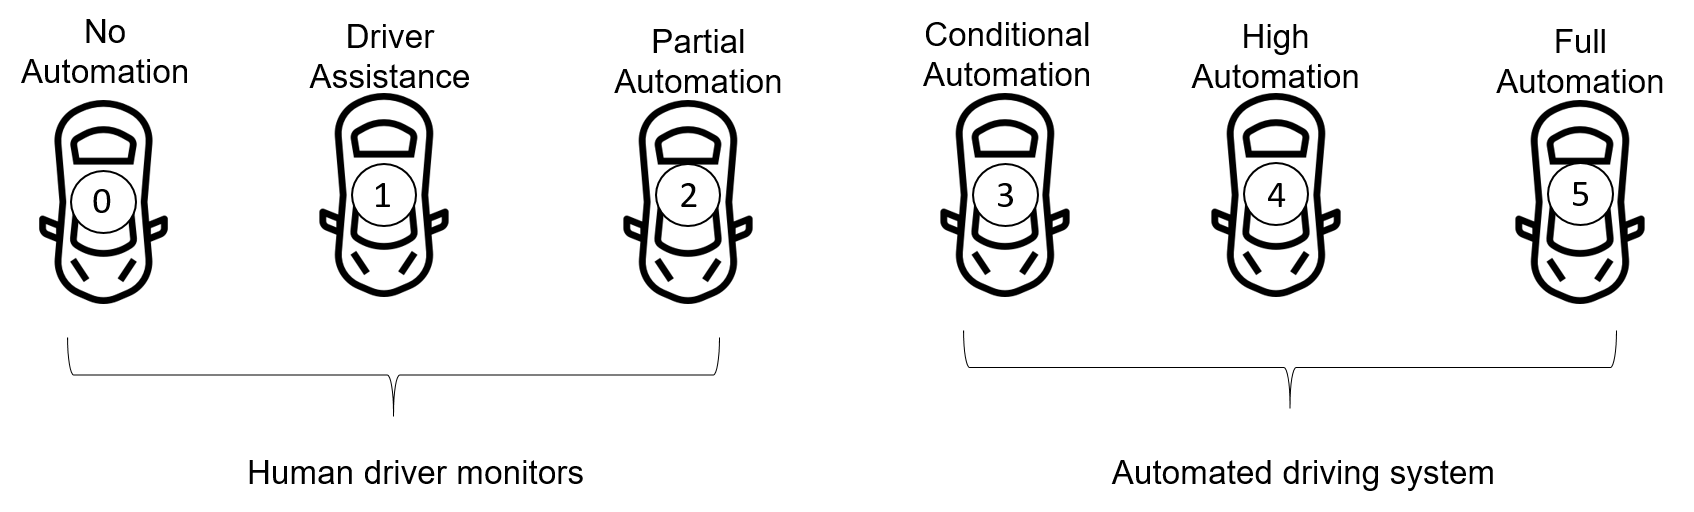
\includegraphics[scale=0.6]{imagens/Levels.png}
\caption{Levels of driving automation}
\label{fig:automation}
\end{figure}

\section{Problem Description}

It is to create an architecture to detect objects and to measure their distance along the road. A possible approach is using drones, but it is not ideal due to the battery life limitation for long tests, as illustrated in Figure \ref{fig:tests}. The goal is to track the position of the cars, namely vehicles under the test (VUT) and traffic simulation vehicles (TSV) along the test track, and send this information to the command central (CC). 

\begin{figure}[H]
\centering
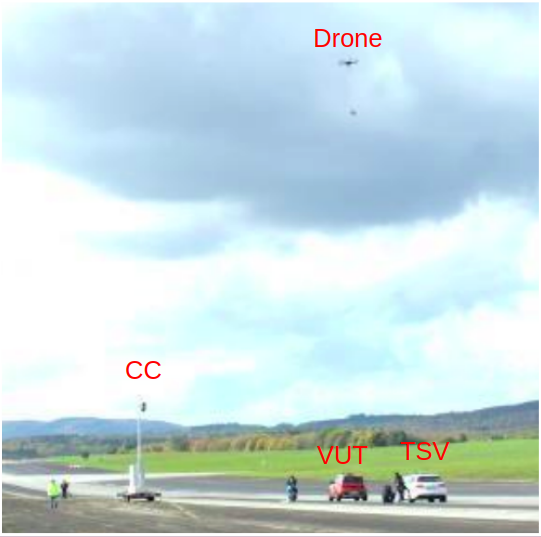
\includegraphics[scale=0.55]{imagens/proposal.png}
\caption{Modelling of the test track scenario using drones, CC designates the command central, VUT is the vehicle under test and TSV is a traffic simulation vehicle.}
\label{fig:tests}
\end{figure}

\section{Objectives}

The main objective is to create a framework to detect objects such as cars, trucks, motorcycles, pedestrians, and other arbitrary obstacles along the road. Additionally, the framework must also be capable of estimating the distance of such objects using a camera array.

\section{Published Works}

Simultaneously, with this work's development, the author has worked in several computer sciences domains, particularly in the data science domain, keeping the multidisciplinary in mind. The following works were published along with the pursuit of the Master's Degree:

\begin{enumerate}

\item \textbf{PRACIANO, BRUNO J. G.}; DE CALDAS FILHO, FRANCISCO L. ; E MARTINS, LUCAS M. C. ; DA CUNHA, DAYANNE F. ; DA SILVA, DANIEL ALVES ; DE SOUSA JÚNIOR, RAFAEL TIMÓTEO. SEGURANÇA DO AMBIENTE USANDO DISPOSITIVO IOT COM PROCESSAMENTO DISTRIBUÍDO. In: Atas da conferência IberoAmericana WWW/Internet 2019, 2019. Atas da conferência Ibero-Americana WWW/Internet 2019, 2019. p. 163

\item MARQUES, Angelica Alves da Cunha; \textbf{PRACIANO, Bruno Justino Garcia}. Researchers of the Brazilian archivistics scientific community in French international areas of interlocution Encontros Bibli: revista eletrônica de biblioteconomia e ciência da informação, Florianópolis, v. 25, p. 01-14, mar. 2020. ISSN 1518-2924. doi:https://doi.org/10.5007/1518-2924.2020.e65864.

\item CASTELINO, R. M.; MOREIRA, G. P.; \textbf{PRACIANO, BRUNO JUSTINO GARCIA}; SANTOS, GIOVANNI A.; WEICHENBERGER, L.; DE SOUSA, JR, RAFAEL T. Improving the accuracy of pedestrian detection in partially occluded or obstructed scenarios. In: 2020 10th International Conference on Advanced Computer Information Technologies, 2020, Deggendorf. 2020 10th International Conference on Advanced Computer Information Technologies, 2020.

\item CANEDO, EDNA; PINHEIRO, GABRIEL; SOUSA JR., RAFAEL; RIBEIRO, RENATO; \textbf{PRACIANO, BRUNO}; LOPES DE MENDONÇA, FÁBIO. Front End Application Security: Proposal for a New Approach. In: 22nd International Conference on Enterprise Information Systems, 2020, Prague. Proceedings of the 22nd International Conference on Enterprise Information Systems, 2020. p. 233.

\item SOUSA JR., RAFAEL; LOPES DE MENDONÇA, FÁBIO; NZE, GEORGES; PINHEIRO, GABRIEL; \textbf{PRACIANO, BRUNO }; CANEDO, EDNA. Performance Evaluation of Software Defined Network Controllers. In: 10th International Conference on Cloud Computing and Services Science, 2020, Prague. Proceedings of the 10th International Conference on Cloud Computing and Services Science, 2020. p. 363.


\item SILVA, DANIEL ALVES DA; TORRES, JOSÉ ALBERTO SOUSA; PINHEIRO, ALEXANDRE; DE CALDAS FILHO, FRANCISCO L.; MENDONÇA, FABIO L. L.; \textbf{PRACIANO, BRUNO J. G}; KFOURI, GUILHERME OLIVEIRA; DE SOUSA, JR, RAFAEL T. Inference of driver behavior using correlated IoT data from the vehicle telemetry and the driver mobile phone. In: 2019 Federated Conference on Computer Science and Information Systems, 2019. org.crossref.xschema.\_1.Title@7d70270b, 2019. p. 487.

\item KFOURI, GUILHERME DE O. ; GONÇALVES, DANIEL G. V. ; DUTRA, BRUNO V. ; ALENCASTRO, JOÃO F. DE ; FILHO, FRANCISCO L. DE CALDAS ; MARTINS, LUCAS M. C. E ; \textbf{PRACIANO, BRUNO J. G.} ; ALBUQUERQUE, ROBSON DE O. ; JR, RAFAEL T. DE SOUSA . Design of a Distributed HIDS for IoT Backbone Components. In: 2019 Federated Conference on Computer Science and Information Systems, 2019. org.crossref.xschema.\_1.Title@7bad8b1f, 2019. p. 81.

\item DE MENDONCA, FABIO L. L.; DA CUNHA, DAYANNE F.; \textbf{PRACIANO, BRUNO J. G.}; DA ROSA ZANATTA, MATEUS; DA COSTA, JOAO PAULO C. L.; DE SOUSA, RAFAEL T. P2PIoT: A Peer-To-Peer Communication Model for the Internet of Things. In: 2019 Workshop on Communication Networks and Power Systems (WCNPS), 2019, Brasilia. 2019 Workshop on Communication Networks and Power Systems (WCNPS), 2019. p. 1.

\item BRANDAO, IURE V.; DA COSTA, JOAO PAULO C. L.; SANTOS, GIOVANNI A.; \textbf{PRACIANO, BRUNO J}. G.; JUNIOR, FRANCISCO C. M. D.; DE S. JUNIOR, RAFAEL T. Classification and predictive analysis of educational data to improve the quality of distance learning courses. In: 2019 Workshop on Communication Networks and Power Systems (WCNPS), 2019, Brasilia. 2019 Workshop on Communication Networks and Power Systems (WCNPS), 2019. p. 1.


\item DO NASCIMENTO SILVA, GERSON ; DE CALDAS FILHO, FRANCISCO LOPES ; DOS REIS, VINICIUS ELOY ; \textbf{PRACIANO, BRUNO JUSTINO }; LUSTOSA, JOÃO PAULO ; DE SOUSA JÚNIOR, RAFAEL TIMÓTEO . MODELO DE REDES NEURAIS ARTIFICIAIS EM SUPORTE TECNOLÓGICO À DETECÇÃO DE CARTEIS EM LICITAÇÕES PÚBLICAS. In: Atas da conferência IberoAmericana WWW/Internet 2019, 2019. Atas da conferência Ibero-Americana WWW/Internet 2019. p. 191.

\end{enumerate}

\section{Chapters Description}

This work is structured as follows: in Chapter 2, the state of the art is presented to support this work, exploring previous contributions in this research area, the theoretical concepts necessary to the understanding of this work, and as self-driving cars are a new trend topic, it is necessary to describe in greater detail.  Chapter 3 shows the proposed framework, and mathematical modeling is presented. Chapter 4 discusses the results achieved, algorithm performance, and the error for object detection and position estimation. Finally, in Chapter 5, the concluding remarks are made regarding the experiments and suggestions of future works.



\chapter{State of the art} \label{capitulo2}

The authors from the paper \cite{Lategahn2013} have presented the next-generation driver assistance systems require precise self-localization. The accuracy of the system is evaluated by computing two independent ego positions of the same trajectory from two distinct cameras and investigating these measures for consistency.

The authors of  \cite{Sankaranarayanan2008} said the video cameras are among the most commonly used sensors in a large number of applications, ranging from surveillance to smart rooms for videoconferencing. In this regard, this paper's primary focus is to highlight the efficient use of the geometric constraints induced by the imaging devices to derive distributed algorithms for target detection, tracking, and recognition.


In \cite{Unlu2019}, the authors said that the drone had seen a tremendous increase in the last few years, making these devices highly accessible to the public. Moreover, Computer vision is extensively used to detect drones autonomously compared to other proposed solutions such as RADAR, acoustics, and RF signal analysis thanks to its robustness. The authors aimed to combine a multi-frame deep learning detection technique, where the frame coming from the zoomed camera on the turret is overlaid on the wide-angle static camera's frame.


In the paper, \cite{Pei2019} was developed three-dimensional coordinates of objects captured by a sequence of images taken in different views. Object reconstruction is a technique that aims to recover the shape and appearance of objects. A novel method to reconstruct occluded objects based on synthetic aperture imaging. The proposed method labels occlusion pixels according to variance and reconstructs the 3D point cloud based on synthetic aperture imaging.


In \cite{Zaarane2020}, the authors proposed an inter-vehicle distance measurement system for self-driving based on image processing. The proposed method uses two cameras mounted as one stereo camera in the hosting vehicle behind the rear-view mirror.  Extensive experiments have shown the high accuracy of the proposed method compared to the previous works from the literature. Also, this method could be used in several systems of various domains in real-time regardless of the object types.

This paper \cite{Wu2019} presented a multi-camera vehicle detection system that significantly improves the detection performance under occlusion conditions. They also inferred the vehicle position on the ground plane by leveraging a multi-view cross-camera context.

In paper \cite{Ali2016}, the authors proposed two approaches: The  Estimation of the distance using an onboard camera and car position detection and vehicle position detection is a method of specifying the relative position to the road can serve as Lane Departure Warning system. 


The authors of \cite{Hane2017} used a surround multi-camera system to cover the full 360-degree field-of-view around the car. Their pipeline can precisely calibrate multi-camera systems, build sparse 3D maps for visual navigation, visually localize the vehicle for these maps, generate accurate dense graphs, and detect obstacles based on real-time depth map extraction.

Unlike existing methods that use pinhole cameras, the implementation of \cite{Cui2019} is based on fisheye cameras whose large field of view benefits various computer vision applications for self-driving vehicles visual-inertial odometry, visual localization, and object detection. To maintain both accuracy and efficiency, while accounting for the fact that fisheye images have a lower angular resolution, we recover the depths using multiple image resolutions. At the end of the pipeline, we fuse the fisheye depth images into the truncated signed distance function volume to obtain a 3D map.

In \cite{Huang2019}, inter-vehicle distance estimation from an in-car camera based on monocular vision is critical.  An improved method for estimating a monocular vision vehicle's distance based on the detection and segmentation of the target vehicle is proposed in this paper to address the vehicle attitude angle problem. The angle regression model is used to obtain the attitude angle information of the target vehicle. The dimension estimation network determines the actual dimensions of the target vehicle.

In \cite{Bao2016}, the multipath and non-line-of-sight effects to GPS receiver decrease the precision of the vehicle's self-localization. More specifically, the lateral error is more severe because of the blockage of the satellites. The lateral distance between building and vehicle estimated by a stereo camera is compared with a 3D building map to rectify the vehicle's lateral position. Besides, this paper employs an inertial sensor and GPS receiver to decide the longitudinal location of the car.

In \cite{Tang2019} introduces CityFlow, a city-scale traffic camera dataset consisting of more than 3 hours of synchronized HD videos from 40 cameras across ten intersections, with the longest distance between two simultaneous cameras being 2.5 km. We expect this dataset to catalyze research in this field, propel the state-of-the-art forward, and lead to deployed traffic optimization in the real world.

In \cite{Qi2019}, the authors measure the distance between the ego-vehicle and the target vehicle by using a monocular vision. They also eliminate estimation error by changing the vehicle pose, proposing a distance estimation method based on the car pose information. The proposed technique can be used to reduce the possible failure of distance estimation produced by changing the inclination angle and roll angle of an unmanned vehicle. Furthermore, the pose information could also help evaluate distance if the car is on a slope.

In paper \cite{Wongsaree2018} presents a distance determination technique using an image from the single forward camera. Therefore, automatic brightness adjustment and inverse perspective mapping are applied in the proposed scheme. The experimental results confirm that the proposed technique can detect the object's distance in front of the car, where the error is 7.96\%.

The paper \cite{Pan2019}, the authors simulated experiments to verify the feasibility of the proposed method. Meanwhile, physical experiment results show that this method can reduce the outdoor environment impact and improve the calibration and measurement precision effectively. Furthermore, In paper \cite{Lin2014} presents a novel method of camera parameters calibration for obstacle distance measurement based on monocular vision. In the end, the experiment shows that the proposed method is advantageous.

In \cite{Simon2019a} the authors have performed experiments on the KITTI dataset for accurate 3D object detection, and they achieved the same results as state-of-the-art in all related categories while maintaining the performance and accuracy trade-off and still run in real-time.


In this paper, we propose weighted-mean YOLO to improve object detection's real-time performance by fusing information of RGB camera and LIDAR. We designed the system using weighted-mean to construct a robust network and compared it with other algorithms. It shows performance improvement of missed-detection \cite{Kim2019}. In paper \cite{Simon2019} introduced the Complex-YOLO, a state of the art real-time 3D object detection network on point clouds only. In this work, they described a system that expands YOLOv2, a fast 2D standard object detector for RGB images, by a specific complex regression strategy to estimate multi-class 3D boxes in Cartesian space. 


In \cite{Oliveira2015}, the method consists of mapping images to a new coordinate system where perspective effects are removed. The removal of perspective associated effects facilitates road and obstacle detection and also assists in free space estimation. As shown in the results, this considerably improves the algorithm's effectiveness and reduces computation time compared with the classical inverse perspective mapping.

The approach introduced by \cite{Salman2017}, a stereo camera, was used, and the calculation of distance considers angular distance, the distance between cameras, and the pixel of the image. They proposed a method that measures object distance based on trigonometry.   

 In \cite{Rangesh2019}, a new framework for tracking multiple objects is presented. They used fusion techniques to achieve this. Second, the purposes of interest are followed directly in the real world. They tested it on real-world highway data collected from a massively sensorized testbed capable of capturing full-surround information.



This paper proposes an intelligent transport system positioning technique that determines the distance between vehicles via image sensor-based visible light communication. A new novel method determines the distance between two cars using a low camera resolution \cite{Tram2018}.


The object detection, classification, and localization in the real world scenario are studied and discussed by \cite{Hofmann2019}. Furthermore, with the opposition, the suggested approach fuses three different algorithms for object detection and classification and uses stereo vision for object localization.  An algorithm for merging the results of the three object detection methods based on bounding boxes is introduced. The proposed fusion algorithm for bounding boxes improves the detection results and provides an information fusion.


\chapter{State of the Art and Technical Background}
\label{capitulo3}

This chapter presents a review of the state of the art in Section \ref{capitulo2}.  An overview of the main concepts of this work. The present section is divided into three sections. In Section \ref{autonomous-vehicles} is defined as the significant concepts of autonomous vehicles. The concepts of sensors are introduced in Section \ref{sensors}. In Section \ref{ml-ai}, the main ideas regarding machine learning and artificial intelligence are described.

\section{State of the art} \label{capitulo2}

This section presents an overview of the related works about this topic. These papers were selected to support the proposed framework during the coding step. These bibliographies support for comparison and the new approach proposal. 

The authors from the paper \cite{Lategahn2013} present the next-generation driver assistance systems that require precise self-localization. The system's accuracy is evaluated by computing two independent ego positions of the same trajectory from two different cameras and investigating them for consistency. The landmark creation of the map is one of the significant contributions to the processing pipeline. The rest of the paper assumes a backward-facing stereo camera setup. Moreover, they calibrated all sensors. And the coordinates transform from camera to receiver to be fully known. Its localization presents on a two-step approach and yields a six degrees of freedom ego pose estimation.

The authors of \cite{Sankaranarayanan2008} state that the video cameras are among the most commonly used sensors in many applications, ranging from surveillance to smart rooms for video conferencing. In this regard, this paper's primary focus is to highlight the efficient use of the geometric constraints induced by the imaging devices to derive distributed algorithms for target detection, tracking, and recognition. The authors introduced the concept of the image's triangulation, and in many detection and tracking applications, once there are correspondences between object locations across views, the localization of these objects in scene coordinates is most important. Each camera gives rise to a line, and estimating the object's location involves computing the point of intersection of these lines. In the presence of noisy measurements, these lines do not intersect at a single point, and error measures such as the sum of squares are used to obtain a robust estimate of the object's location \cite{hartley1997triangulation}.

In \cite{Unlu2019} the authors remark that the use of drones has seen a tremendous increase in the last few years, making these devices highly accessible to the public. Besides, computer vision is widely used to autonomously detect drones contrasted to other proposed solutions such as RADAR, acoustics, and RF signal analysis, due to its robustness. The authors aimed to combine a multi-frame deep learning detection method, where the frame coming from the zoomed camera on the turret is overlaid on the wide-angle static camera's frame. Their equipment's nature can group the proposed approaches in the market and academic papers. However, conventional ones cannot detect small commercial uncrewed aerial vehicles. Also, they are flying at relatively much lower velocities, which decreases the Doppler signature. Based on this information, the authors proposed an approach based on cameras.

The paper \cite{Pei2019} shows the development of a three-dimensional coordinate system of objects captured by a sequence of images taken in different views. Object reconstruction is a technique that aims to recover the shape and appearance of items. A novel method to reconstruct occluded objects based on synthetic aperture imaging is presented. The proposed method labels occlusion pixels according to variance and reconstructs the 3D point cloud based on synthetic aperture imaging.

In \cite{Zaarane2020} the authors propose an inter-vehicle distance measurement system for self-driving based on image processing. The proposed method uses two cameras mounted as one stereo camera in the rear-view mirror's hosting vehicle.  Extensive experiments have shown the proposed method's high accuracy compared to the previous works from the literature. This method could also be used in several systems of various domains in real-time regardless of the object type. The paper \cite{Wu2019} presents a multi-camera vehicle detection system that significantly improves the detection performance under occlusion conditions. They also infer vehicle position on the ground plane by leveraging a multi-view cross-camera context.

In the paper \cite{ Ali2016}, the authors proposed two approaches: estimation of distance using an onboard camera, car position detection, and vehicle position detection is a method of specifying the relative position to the road that can serve as a Lane Departure Warning system. The authors of \cite{Hane2017} used a surround multi-camera system to cover the full 360-degree field-of-view around the car. Their pipeline can precisely calibrate multi-camera systems, build sparse 3D maps for visual navigation, visually localize the vehicle for these maps, generate accurate dense graphs, and detect obstacles based on real-time depth map extraction.

Unlike existing methods that use pinhole cameras, the implementation of \cite{Cui2019} is based on fisheye cameras, whose large field of view benefits various computer vision applications for self-driving vehicles visual-inertial odometry, visual localization, and object detection. It recovers the depths using multiple image resolutions. At the end of the pipeline, the authors fuse the fisheye depth images into the truncated signed distance function volume to obtain a 3D map.

In \cite{Huang2019}, the authors show that inter-vehicle distance estimation from an in-car camera based on monocular vision is critical.  An improved method for estimating a monocular vision vehicle's distance based on the target vehicle's detection and segmentation is proposed in this paper to address the vehicle attitude angle problem. The angle regression model is used to obtain the attitude angle information of the target vehicle. The dimension estimation network determines the actual dimensions of the target vehicle.

In \cite{Bao2016}, the multipath and non-line-of-sight effects of GPS receivers decrease the precision of the vehicle's self-localization. More specifically, the lateral error is more severe because of the blockage of the satellites. The lateral distance between building and vehicle estimated by a stereo camera is compared with a 3D building map to rectify its lateral position. Besides, this paper employs an inertial sensor and GPS receiver to decide the car's longitudinal location.

In \cite{Tang2019} introduces CityFlow, a city-scale traffic camera dataset consisting of more than 3 hours of synchronized HD videos from 40 cameras across ten intersections, with the longest distance between two simultaneous cameras being 2.5 km. The authors expected this dataset to catalyze research in this field, propel the state-of-the-art forward, and lead to deployed traffic optimization in the real world.

In \cite{Qi2019}, the authors measure the distance between the ego-vehicle and the target vehicle using a monocular vision. They also eliminate estimation error by changing the vehicle pose, proposing a distance estimation method based on the car pose information. The proposed technique can reduce the possible failure of distance estimation produced by changing an uncrewed vehicle's inclination angle and roll angle. Furthermore, the pose information could also help evaluate distance if the car is on a slope.

In paper \cite{Wongsaree2018}, a distance determination technique using an image from the single forward camera is presented. Therefore, automatic brightness adjustment and inverse perspective mapping are applied in the proposed scheme. The experimental results confirm that the proposed technique can detect the object's distance in front of the car, where the error is 7.96\%.

The paper \cite{Pan2019} simulated experiments to verify the feasibility of the proposed method. Meanwhile, physical experiment results show that this method can effectively reduce the outdoor environment impact and improve the calibration and measurement precision. Furthermore, in \cite{Lin2014} presents a novel method of camera parameters calibration for obstacle distance measurement based on monocular vision, and the experiment shows that the proposed method is advantageous.

In \cite{Simon2019a}, the authors performed experiments on the KITTI dataset for accurate 3D object detection. They achieved the same results as state-of-the-art in all related categories while maintaining the performance and accuracy trade-off and still run in real-time.


This paper weighted-mean YOLO to improve object detection's real-time performance by fusing RGB cameras and LIDAR information. It implemented a new system using weighted-mean to construct a robust network and compared it with other algorithms. It shows performance improvement of missed-detection \cite{Kim2019}. In paper \cite{Simon2019} introduced the Complex-YOLO, a state of the art real-time 3D object detection network on point clouds only. This work describes a system that expands YOLOv2, a fast 2D standard object detector for RGB images, by a specific complex regression strategy to estimate multi-class 3D boxes in Cartesian space. 

In \cite{Oliveira2015}, the proposed method consists of mapping images to a new coordinate system where perspective effects are removed. The removal of perspective associated effects facilitates road and obstacle detection and also assists in free space estimation. The results show this considerably improves the algorithm's effectiveness and reduces computation time compared with the classical inverse perspective mapping.

In \cite{Salman2017}, a stereo camera calculated the distance considering the angular distance, the distance between cameras, based on the image's pixel. They proposed a method that measures object distance based on trigonometry.  In \cite{Rangesh2019}, a new framework for tracking multiple objects is presented. They used fusion techniques to achieve this. They tested it on real-world highway data collected from a massively sensorized testbed capable of capturing full-surround information.

In \cite{Tram2018}, a new intelligent transport system positioning technique that determines the distance between vehicles via image sensor-based visible light communication was implemented. An original novel method determines the distance between two cars using a low camera resolution.

The object detection, classification, and localization in the real world scenario are studied and discussed by \cite{Hofmann2019}. Furthermore, the suggested approach fuses three different object detection algorithms and classification and uses stereo vision for object localization with the opposition. An algorithm for merging the results of the three object detection methods based on bounding boxes is introduced. The proposed fusion algorithm for bounding boxes improves the detection results and provides an information fusion.



\section{Technical Background}
This section contains the technical background necessary for this thesis understanding. It is divided into three subsections: the concepts behind autonomous vehicles, sensors, and machine learning.

\subsection{Autonomous Vehicles} \label{autonomous-vehicles}

This section discusses the importance of the autonomous vehicles domain and its applicability to the society, and the problems occurred as well. 

\subsubsection{What are autonomous vehicles}
Modern vehicles now have Advanced Driver Assistance Systems (ADAS)
which work at several levels of autonomy, with these levels being
outlined by the National Highway Traffic Safety Administration
(NHTSA). The levels range from 0, no-automation, to 5, full self-driving automation \cite{national2013preliminary}. An example of an ADAS is a parking system, proposed by \cite{krasner2016automatic}, that uses sensors to find the best way to maneuver a car into a parking space without driver input. Systems such as these are being used in modern semi-autonomous
vehicles as driver aids to hand over work from the driver to the
car’s systems \cite{schoning2006parklenkassistent}. As technology progresses, there will be a more
and more handover of control from the driver to the vehicle, level
Four of automation being the fully-autonomous state that is a main talking point in the automotive industry. The level 5 AV will
be able to self-drive anywhere ("full automation"), i.e., no cockpits,
drivers are not required to be fit to drive, and even they do not require a driving license (every person in a vehicle is a passenger).

There are many open datasets to allow new people to work with autonomous vehicles and hackathons as well. In the special the KITTI Dataset \cite{geiger2013vision} and NuScenes in \cite{caesar2020nuscenes}. These datasets provided data using GPS, Camera, RADAR, and LIDAR. 

\subsubsection{Challenges in Autonomous Vehicles}

The cities are not prepared for autonomous vehicles at the same velocity as the industry. Based on the data provided by \cite{cutler2015many}, only 6\% of the biggest cities in the United States are considering creating the necessary infrastructure to work with this new reality.

Putting autonomous vehicles on the street is prolonged due to other problems taking care of the network issues, even 3G, 4G, or 5G, the roads' conservation, and the most critical aspect regarding the legislation. 

The study and development of these applications will change many things in society, even in the process sector, until companies work with delivery. Nevertheless, it is indispensable to control the traffic and reduce the accidents, It follows the World Health Organization (WHO), every year, over 1 million people lose their lives in car accidents, and only in Brazil is over 47,000 deaths \cite{world2004world}. 





\subsection{Sensors}\label{sensors}

Figure \ref{fig:autonomous-vehicles} shows the correct place for the principal sensors of an autonomous vehicle, model Audi A8 \cite{ross2017audi}. The subsections \ref{sub:camera}, \ref{sub:radar}, and
\ref{sub:lidar} describe camera, radar, and LiDar respectively. 

Autonomous vehicles (AV) would be impossible without sensors: they allow the car to see and sense everything on the road and collect the information needed to drive safely \cite{kocic2018sensors}. Furthermore, this information is processed and analyzed to build a path from point A to point B and send the appropriate instructions to the car's controls, such as steering, acceleration, and braking \cite{kato2015open}.

The technology of sensor manufacturing has shown a significant evolution in the last years, having the appearance of a great diversity of sensors and a general decrease in its cost. Thus, from an economic point of view, it became interesting to replace a high-precision, high-cost sensor with several low-cost and less accurate sensors \cite{varghese2015overview}. The combination of multiple low-cost sensors also implied the development of new methods for merging data from various sensors and specific electronics with high processing capacity capable of using the advantages of these new sensors and minimizing their low precision deficiencies \cite{krasniqi2016use}.


\begin{figure}[H]
\centering
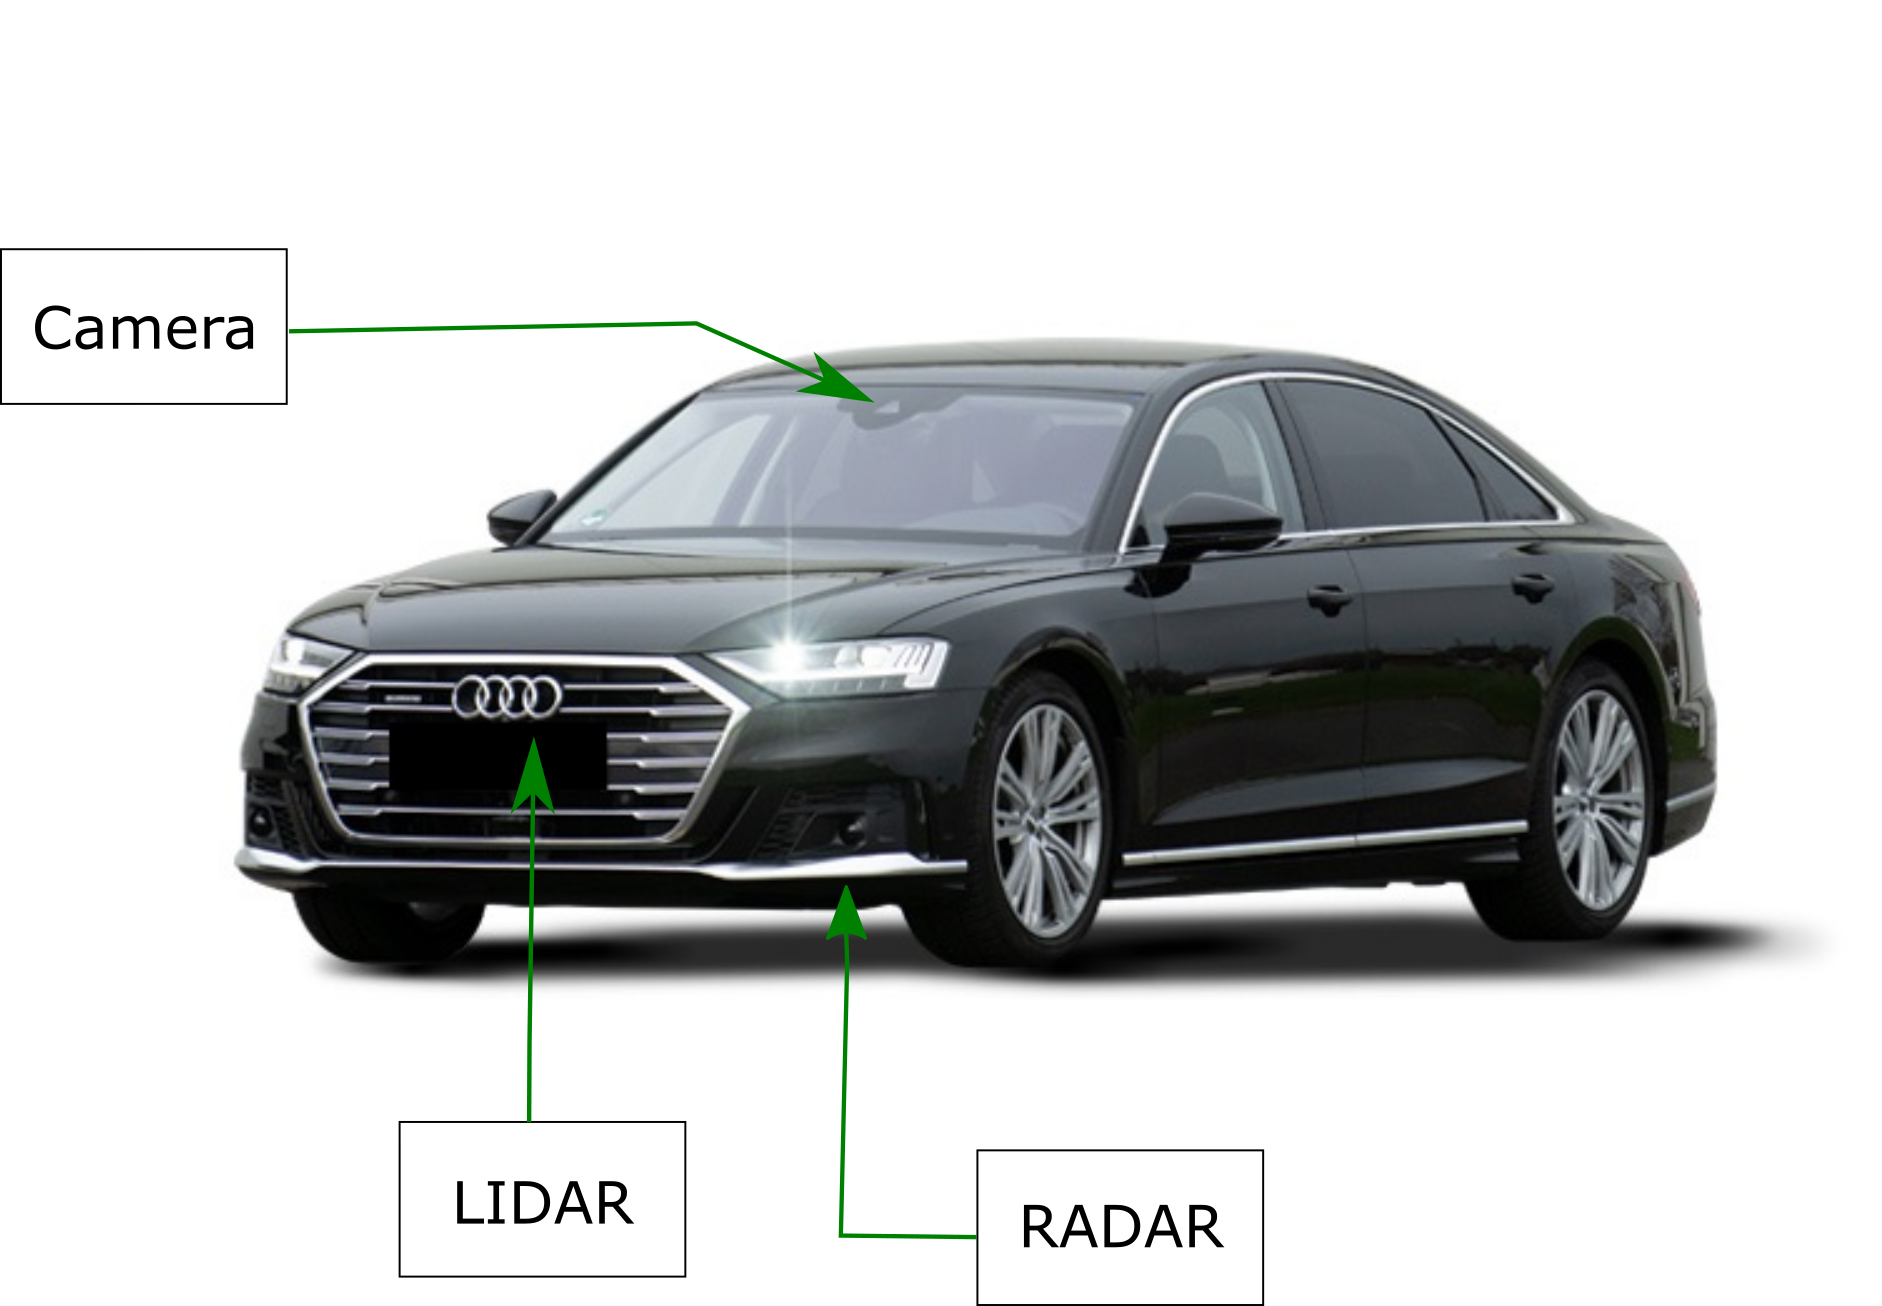
\includegraphics[scale=0.6]{imagens/image823.png}
\caption{Representation of an autonomous vehicle}
\label{fig:autonomous-vehicles}
\end{figure}


Each sensor has a different range and coverage angle, and this mixing of the sensor in the car allows it to cover a big area and make it possible to reduce car accidents and improve the driver's safety.  Although Figure \ref{fig:sensorsrange} shows reasonable performance parameters for AV sensors, specific sensor designs, and implementations will ultimately determine the performance parameters for a particular AV in the real world.


\begin{figure}[H]
\centering
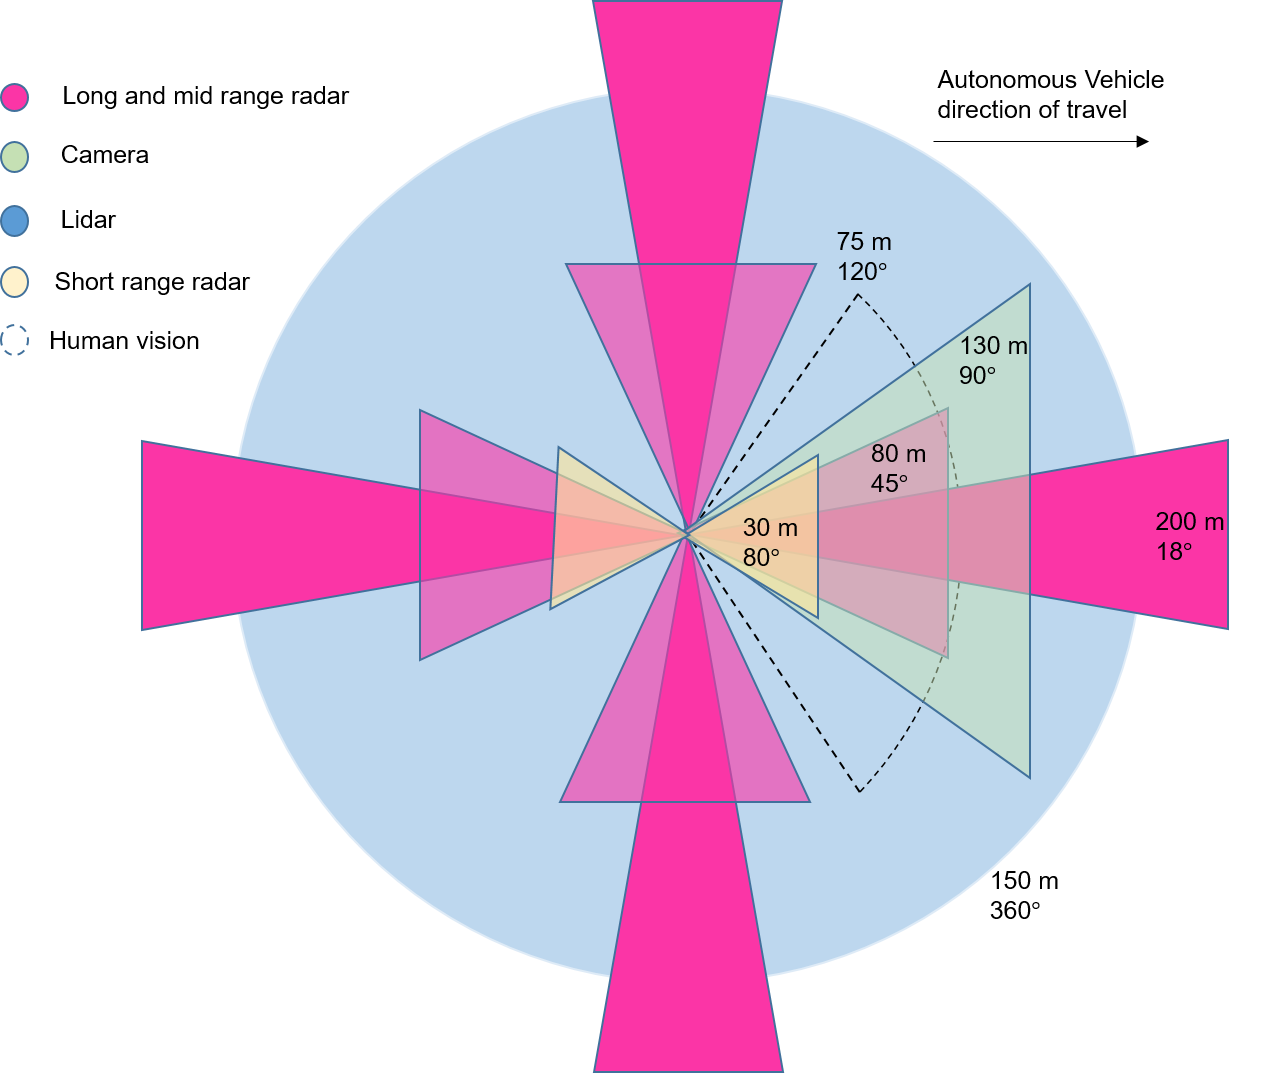
\includegraphics[scale=0.5]{imagens/Imagem1.png}
\caption{Illustration of the various sensors, with reasonable estimates of coverage area (field of view) and typical operating ranges}
\label{fig:sensorsrange}
\end{figure}



\subsubsection{Camera}\label{sub:camera}
The camera is the type of sensor that allows the car to perceive the environment using the collected images. Figure \ref{fig:camera} shows the standard camera for autonomous vehicles.

It is an optical instrument for image or video capture in the same size. For example, there are some cameras where it is possible to set up the numbers of frames per second (FPS) and the image resolution. 

It is also essential to remember the importance of the camera's calibration; the Equations for this process were available in \cite{888718}. This step is necessary to acquire the objects' real size because it is sometimes required to compare these objects' dimensions. 

\begin{figure}[H]
\centering
\includegraphics[width=80mm]{imagens/camera.png}
\caption{Representation of a camera of the autonomous vehicle \cite{site-camera}}
\label{fig:camera}
\end{figure}

There are many different models of cameras, which vary in their technical specs. In this thesis, it uses GoPro5, which is the highest-end model. The camera alone weighs 118 g and 186 g with the camera. We selected this camera because it works better for outside scenarios. GoPro gives the user great control of the settings for both picture and video acquisition. Video offers some recording options, from 480p until 4k resolution, at various frame rates. There is also the option to shoot in 4K—a resolution higher than most HD televisions. The user can also adjust exposure, white balance, color, ISO, and sharpness, among other settings \cite{paro2015video}.

GoPro carries a WiFi signal within itself that allows connected devices like another GoPro or your computer. There is no internal storage, and video is saved into removable microSD cards. Battery life is dependent on which video quality. The official Web site suggests a battery life of 2 hours of continuous video and three hours for recharging.

This sensor allows the car to detect many objects while it is possible to perform object recognition. It is necessary to freeze the difference between object detection and object recognition. There are different algorithms to perform these tasks. The proposed algorithm in Chapter \ref{capitulo4} shows both exposures combined with the estimation of the distance. 

\subsubsection{Radar}\label{sub:radar}

The automotive radio detection and ranging (RADAR) sensors are responsible for performing object detection around the vehicle and avoiding potential collisions. Therefore, with this sensor, it is possible to warn the driver and combined with level 1 of automation, as shown in Figure \ref{fig:automation}, to intervene with the brake the car or use other controls to prevent an accident \cite{ariyur2006collision}.

\begin{figure}[H]
\centering
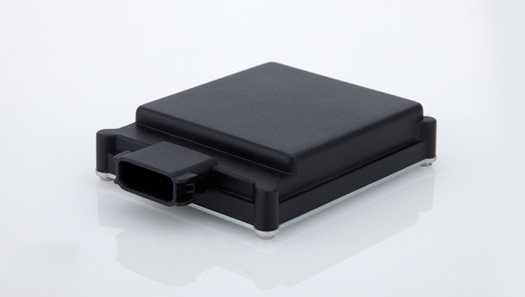
\includegraphics[width=120mm]{imagens/radar.jpg}
\caption{A commercial radar model ARS430 CV from Continental}
\label{fig:camera}
\end{figure}

Another exciting application of the RADAR in the automotive scenario is measuring the vehicle's relative speed and other objects. It is possible to estimate the distance correctly  \cite{stevenson2011long}.

It is possible to combine the camera and RADAR and get a new kind of sensor, as defined in \cite{kamerad}. With this approach, it is possible to reach 160 times faster than a human driver.

\subsubsection{Lidar}\label{sub:lidar}
In Figure \ref{fig:lidar} is shown a light detection and ranging (LiDAR). The main purpose of this laser is to detect and track any kind of objects. 
\begin{figure}[H]
\centering
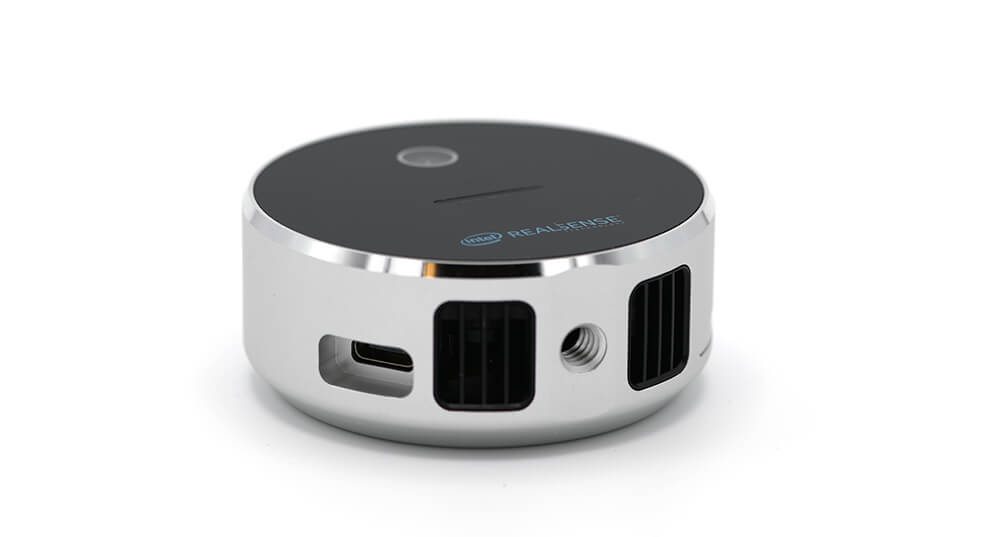
\includegraphics[scale=0.25]{imagens/lidar.jpg}
\caption{An exemple of a lidar of the autonomous vehicle}
\label{fig:lidar}
\end{figure}

This measurement is based on many times rotate this sensor in different directions to scan the whole area of the autonomous vehicles is driving and collect some data for detecting the objects \cite{gao2018object}.

The name is similar to Radar is not a coincidence. The two technologies exist to understand what is happening in the environment around them, but their methods are different.

The Radar transmits radio waves from a receiver. The radio waves then bounce off objects in the receiver's vicinity to detect how and where said objects are moving. It is available angle and velocity, things of that nature. Think of a weather radar, which measures how quickly and in what direction a storm cloud is moving. 

This sensor shoots out invisible beams of light from across the light spectrum. It can use infrared and ultraviolet light to map out the environment around it. It can get a sense of both the physical dimensions and motion (if any) of objects in its vicinity. The usage of the LiDAR is a way to figure out the environment around the object using laser beams.  

Autonomous vehicles may use Lidar for object detection and to navigate safely through environments \cite{Lim2019}. Point cloud output from the Lidar sensor provides the necessary data for automated software to determine potential obstacles in the ground and where the robot is concerning those potential obstacles.  such as CARLA simulator \cite{dosovitskiy2017carla}\cite{dworak2019performance}.

\section{Machine Learning in Computer Vision}\label{ml-ai}
The machine learning is an approach based on algorithms to create some predictions. These techniques are based on mathematical and computer science. It is possible to apply this in several fields of science. 
\subsection{Artificial Neural Networks}

The human brain has inspired artificial neural networks (ANN) or perceptron. This approach is because of the capacity of the human mind to categorize new information. In Figure \ref{fig:ann} is shown an example of the structure of an ANN. There is an input array with the processed features for categorization. The next step of the processing is to define the weights for this analysis. The activation function is the central part of this process. In this step, the algorithm will transform the numbers collected by the previous actions and return only in twofold purpose, like $0$ and $1$ in the output layer \cite{goodfellow2016deep}.

\begin{figure}[H]
\centering
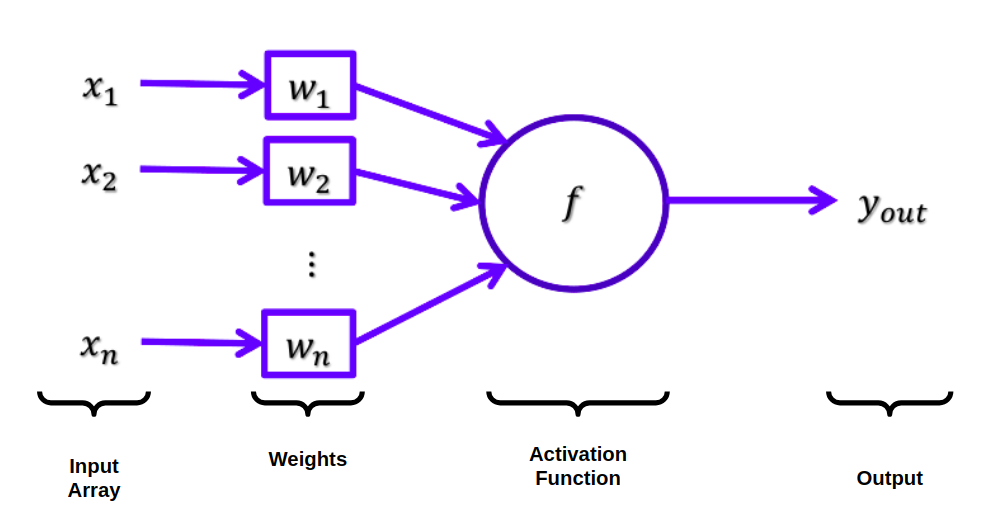
\includegraphics[width=\columnwidth]{imagens/ann.png}
\caption{The structure of an ANN \cite{lecture}}
\label{fig:ann}
\end{figure}

The neuron output is a function of the weighted sum of its inputs. Figure \ref{fig:ann_weight} is shown the mathematical background, where $f$ is activation function, $w_i$ are the weights, and $\beta$ is the constant input called bias.


\begin{figure}[H]
\centering
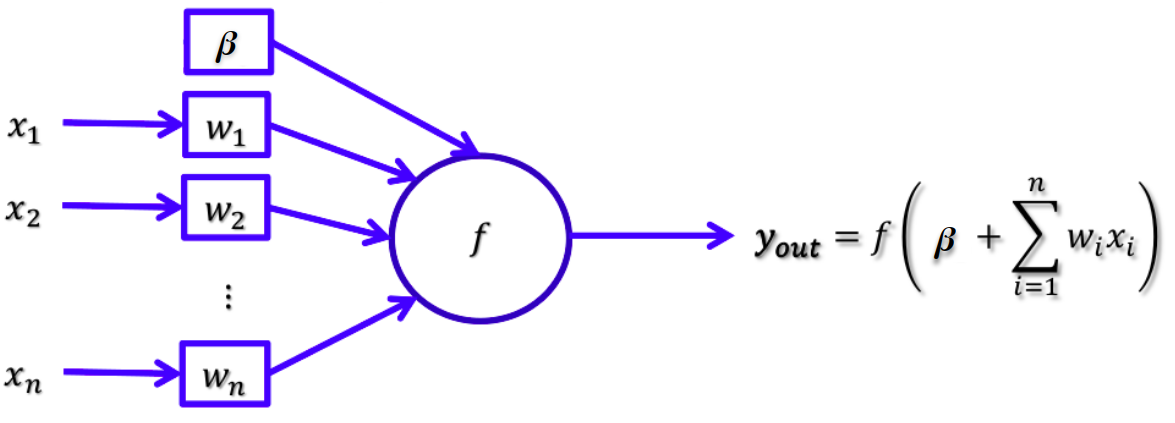
\includegraphics[width=\columnwidth]{imagens/math_ann_bias.png}
\caption{Mathematical representation of ANN with bias \cite{lecture}}
\label{fig:ann_weight}
\end{figure}


\subsubsection{Activation functions}
There are many different activation functions to use. These are crucial for ANN characteristics, such as learning ability and computational efforts in training and validation.

There are different kinds of activation functions for machine learning approaches. Each activation function has its particularity for specific problems. Table \ref{tab:tab1} shows the characteristics for these functions. 


\begin{table}[H]
\caption{Comparison Table for Activation Functions}
\centering
\resizebox{15.3cm}{!}{%
\begin{tabular}{|c|c|c|c|c|c|c|}
\hline
\textbf{\begin{tabular}[c]{@{}c@{}}Activation\\ Function\end{tabular}}  & \textbf{Linear}          & \textbf{Monotonic} & \textbf{Continuous}      & \textbf{\begin{tabular}[c]{@{}c@{}}Derivative \\ Monotonic\end{tabular}} & \textbf{\begin{tabular}[c]{@{}c@{}}Derivative\\ Continuous\end{tabular}} & \textbf{\begin{tabular}[c]{@{}c@{}}Simetric with \\ respect to \\ The Origin\end{tabular}} \\ \hline
{\color[HTML]{000000} Unit Step} & {\color[HTML]{FE0000} x} & {\color[HTML]{009901} \checkmark}& {\color[HTML]{FE0000} x} & {\color[HTML]{FE0000} x} & {\color[HTML]{FE0000} x} & {\color[HTML]{FE0000} x} \\ \hline
Sign & {\color[HTML]{FE0000} x} & {\color[HTML]{009901} \checkmark}& {\color[HTML]{FE0000} x} & {\color[HTML]{FE0000} x} & {\color[HTML]{FE0000} x} & {\color[HTML]{009901} \checkmark} \\ \hline
Identity & {\color[HTML]{009901} \checkmark}& {\color[HTML]{009901} \checkmark}& {\color[HTML]{009901} \checkmark}& {\color[HTML]{FE0000} x} & {\color[HTML]{009901} \checkmark}& {\color[HTML]{009901} \checkmark}\\ \hline
Sigmoid                                                                 & {\color[HTML]{FE0000} x} & {\color[HTML]{009901} \checkmark}             & {\color[HTML]{009901} \checkmark}                   & {\color[HTML]{FE0000} x}                                                 & {\color[HTML]{009901} \checkmark}                                                                   & {\color[HTML]{FE0000} x}                                                               \\ \hline
\begin{tabular}[c]{@{}c@{}}Hyperbolic\\ Tangent\end{tabular}            & {\color[HTML]{FE0000} x} & {\color[HTML]{009901} \checkmark}             & {\color[HTML]{009901} \checkmark}                   & {\color[HTML]{FE0000} x}                                                 & {\color[HTML]{009901} \checkmark}                                                                   & {\color[HTML]{009901} \checkmark}                                                                                 \\ \hline
\begin{tabular}[c]{@{}c@{}}Rectified \\ Linear Unit \\ (ReLU)\end{tabular} & {\color[HTML]{FE0000} x} & {\color[HTML]{009901} \checkmark}              & {\color[HTML]{009901} \checkmark}                   & {\color[HTML]{009901} \checkmark}                                                                   & \begin{tabular}[c]{@{}c@{}}{\color[HTML]{FE0000} x}\\ (at 0)\end{tabular}                       & {\color[HTML]{FE0000} x}                                                               \\ \hline
\end{tabular}\label{tab:tab1}}
\end{table}


Equation \ref{eq:eq_unit} shows the behavior of the Unit Step activation function ($H(x)$) where it is possible to note that it is nonlinear, monotonic, and adequate for classification. However, on the other hand, it has discontinuous derivatives and not monotonic with gradient descent methods.


\begin{equation}\label{eq:eq_unit}
    H(x) = \left\{\begin{matrix}
    1 & if & x >  0,\\
    \frac{1}{2} & if & x = 0, \\
    0 & if & x < 0 
    \end{matrix}\right.
\end{equation}

Equation \ref{eq:sign} shows the behavior of the Sign Function activation function. Its properties are similar to the (\ref{eq:eq_unit}) as they have, essentially, the same format with different values. The pros are nonlinear, monotonic, and ideal for fine classification, but the cons are discontinuous and not suitable for regressions.


\begin{equation}\label{eq:sign}
    sgn(x) = \left\{\begin{matrix}
    1 & for & x >  0,\\
    0 & for & x = 0, \\
    -1 & for & x < 0 
    \end{matrix}\right.
\end{equation}

        


Equation (\ref{eq:identity}) defines the Identity activation function where the usage is indicated when necessary to optimize the weights, but for multilayers networks are not recommended because it is a linear function. 


\begin{equation}\label{eq:identity}
    f(x) = x
\end{equation}


Equation (\ref{eq:sigmoid}) shows the classic activation function for the multi-layer networks. It is important to remind that this function is nonlinear, monotonic, and well-suited to gradient descent, but its asymmetry to the origin may have slower convergence and can get stuck at the training time.     


\begin{equation}\label{eq:sigmoid}
    \mathrm{S}(x) = \frac{1}{1+e^{-x}}
\end{equation}

        
Equation (\ref{eq:hiper}) proposes an alternative to (\ref{eq:sigmoid}) where has a non-linearity and it is symmetric to its origin, and it is well suited to gradient descent optimization, but at the same, it does not have a monotonic derivative and can have a slow convergence, but it is better sometimes than the Sigmoid activation function.


\begin{equation}\label{eq:hiper}
 \mathrm{tanh}(x) = \frac{e^{x}-e^{-x}}{e^{x}+e^{-x}}
\end{equation}


    


In this work, ReLU is the activation function chosen activation. Its mathematical definition is shown in (\ref{eq:relu}). This activation function is a novel, and it is widely used in deep networks because it is nonlinear and has a fast convergence. Contrarily to the previous equations, it is not differential continuously just at zero, and the issues to work with gradient descent is just around the origin. 


\begin{equation}
\label{eq:relu}
    f(x) = \mathrm{R}(x) = \mathrm{max}(0,x)
\end{equation}


The graphic visualization of the function Relu is shown in Figure \ref{fig:relu}, where this function returns $0$ if the number from the weighted sum is lower than $0$, or return $x$ if the previous value is over than $0$.


\begin{figure}[H]
\centering
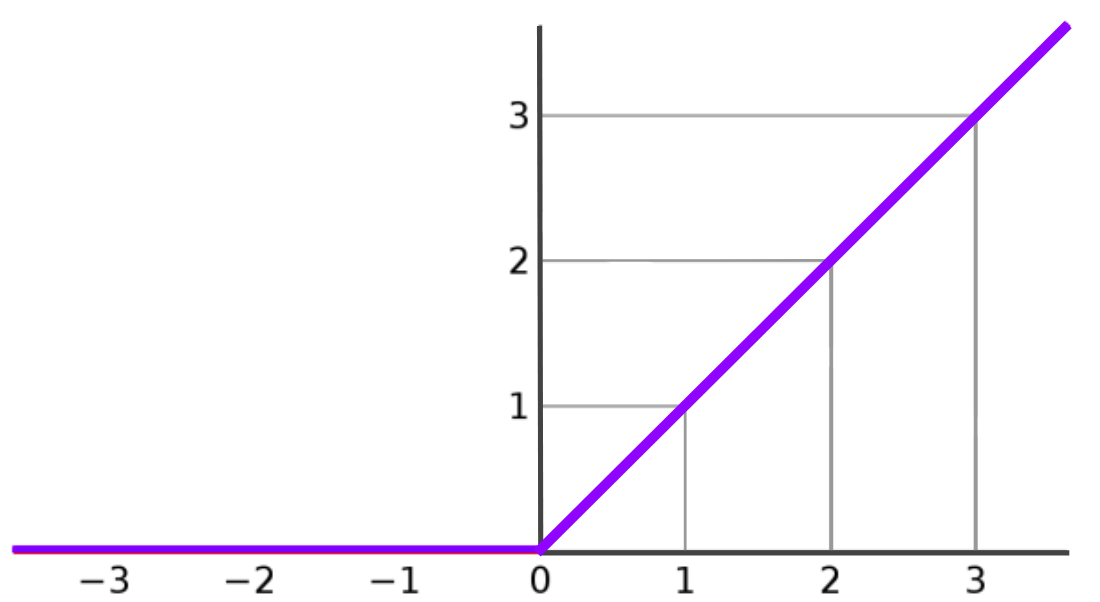
\includegraphics[scale=0.2]{imagens/relu_corrected.png}
\caption{The behavior of the Relu \cite{lecture}}
\label{fig:relu}
\end{figure} 

These are the essential characteristics of this activation function. It is widely used in deep networks. It is nonlinear, monotonic, derivative monotonic, and fast converge. As the weaknesses, this activation function has a non continuously differential at zero, i.e., issues with gradient descent around the origin.



\subsubsection{Layered Neural Networks}

The quintessential element of a deep learning model is the multilayer perceptron (MLP) ~\cite{goodfellow2016deep}. An MLP is just a mathematical function mapping some set of input values to output values. The function
is formed by composing many more specific functions \cite{goodfellow2016deep}.


These are important deep learning models. The goal
of a feedforward network is to approximate some function $f*$. For example, for a classifier, $y = f*(x)$ maps an input x to a category y. A feedforward network
defines a mapping $y = f (x; \theta)$ and learns the value of the parameters $\theta$ that result in the best function approximation.

These models are called feedforward because information flows through the function being evaluated from $x$, through the intermediate computations used to define $f$, and finally to the output $y$. There are no feedback connections in which results of the model are fed back into itself.



\subsection{Convolutional Neural Networks}\label{sec:cnn}


The Convolutional Neural Networks (CNN) is a specialized neural network for processing data known as in \cite{lecun1995convolutional}. For example, in the autonomous vehicle domain, this approach is several used for object detection and object identification. This name  indicates that the network employs a mathematical operation called
convolution. 

A CNN coarsely scans the image for features (in lower dimension space), pools possible patterns, then inspect those patterns in detail with its fully connected
subnetworks, generating their classifications. In Figure \ref{fig:cnn_car} is defined the full process of this neural network. Where there are three other importants is steps: Convolutional layer is defined in Subsection \ref{sub:conv}. The pooling layer is introduced in the Subsection \ref{sub:pooling}.
\begin{figure}[H]
\centering
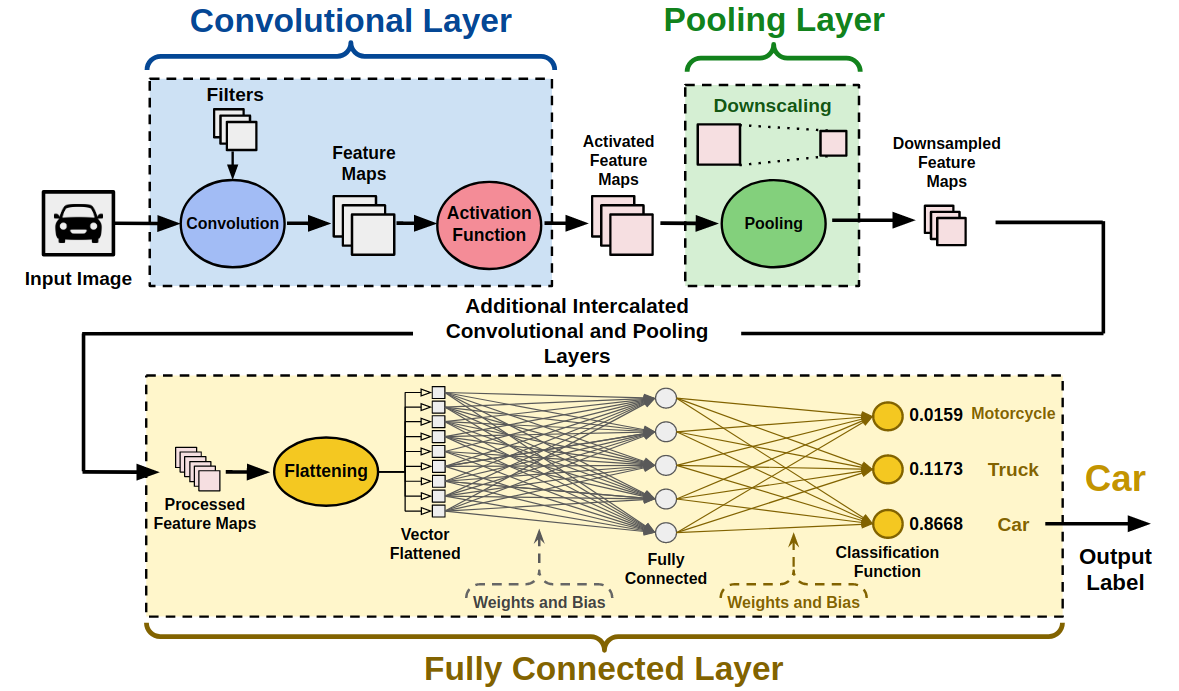
\includegraphics[width=\columnwidth]{imagens/Full_Process.png}
\caption{Full process of a convolutional neural network \cite{lecture}}
\label{fig:cnn_car}
\end{figure}


\subsubsection{Convolutional Layer}
\label{sub:conv}

The standard inputs are a tridimensional matrix with height and width defined accordingly with the image dimensions and determined by the number of colors. In general, the images use three color channels, Red-Green-Blue (RGB), as is shown in Figure \ref{fig:rgb}.

\begin{figure}[H]
\centering
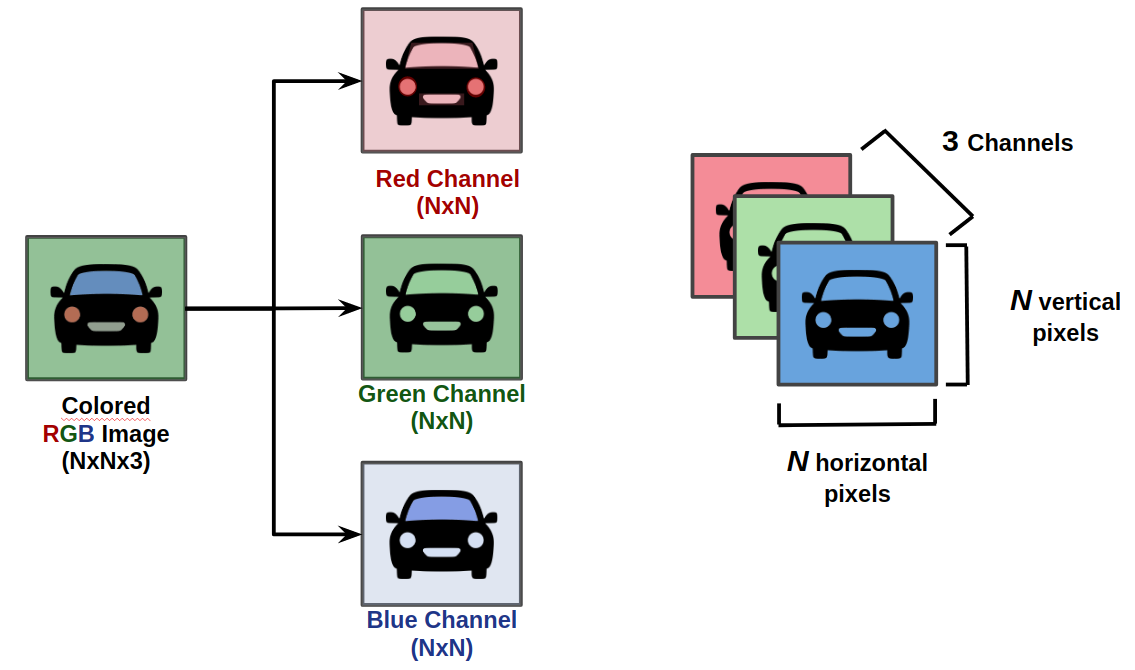
\includegraphics[scale=0.35]{imagens/rgb_representation.png}
\caption{Representation of the colors of the input image \cite{lecture}}
\label{fig:rgb}
\end{figure}


The convolutions work as filters that seem little squares, and they are slipping through the whole image and capturing essential parts.  Figure \ref{fig:bias} shows an image by dimensions of $NxNX3$, filter among the $MxMX3$, wherever individual main difference per result is then summed, on bias ($\beta$) value, then passed through an activation function. Furthermore, the end of the process generates a new matrix called a feature map or activation map.


\begin{figure}[H]
\centering
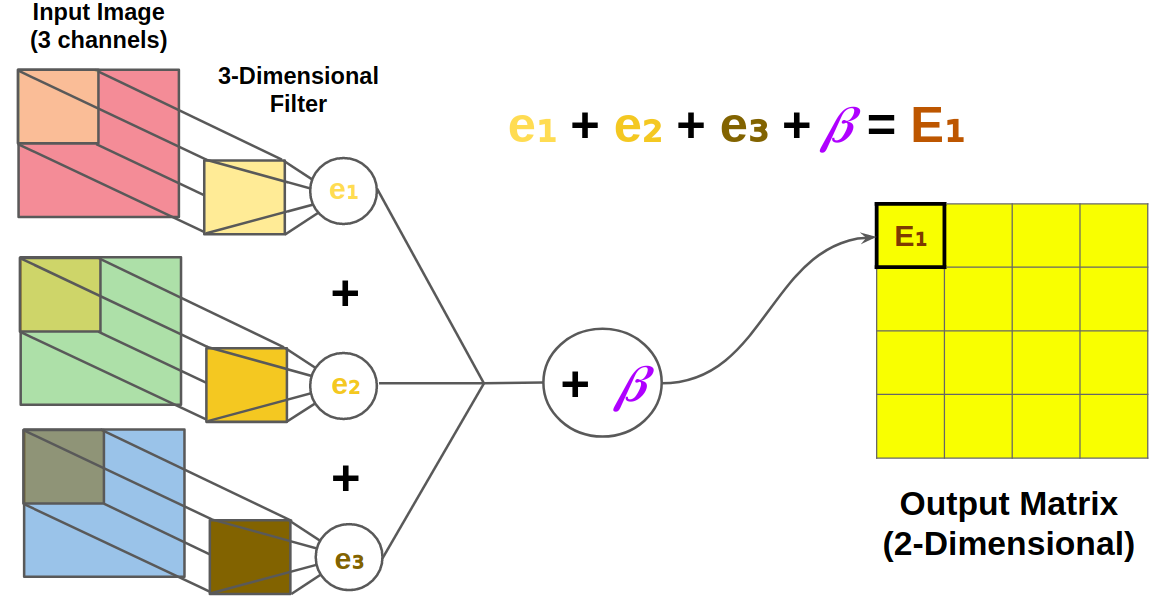
\includegraphics[scale=0.3]{imagens/three_dim_conv_2.png}
\caption{Representation of the convolution process \cite{lecture}}
\label{fig:bias}
\end{figure}




\subsubsection{Pooling and Upsampling}\label{sub:pooling}

A pooling layer is necessary to simplify the information from the previous layer. The convolution layer chooses a unit area, for example, $2x2$, to slicing for the whole output information from the previous step. To brief, if the information from the previous layer was $4x4$, the output from the process of pooling will be $2x2$. Nevertheless, the most used method is max-pooling, where the biggest number in the matrix is passed to the next step. This data summarization is used to reduce the number of weights and avoid overfitting. In Figure \ref{fig:pooling} is shown the max-pooling process.

\begin{figure}[H]
\centering
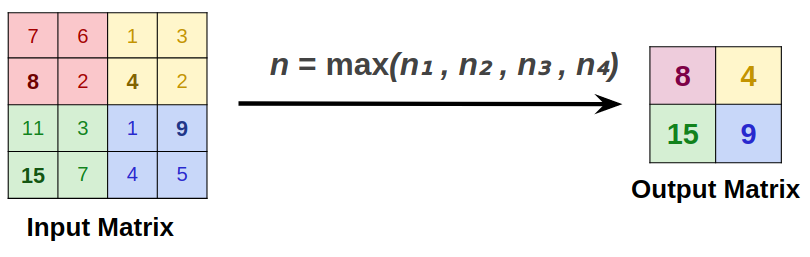
\includegraphics[scale=0.35]{imagens/max_pooling.png}
\caption{Representation of the maxpooling process \cite{lecture}}
\label{fig:pooling}
\end{figure}




\subsubsection{Auto-encoders}\label{auto-encoder}

It is a special type of neural network that is used to copy its inputs to its output. The intern structure is defined in Figure \ref{fig:autoencoder}. 

\begin{figure}[H]
\centering
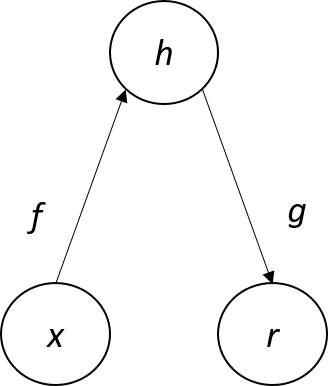
\includegraphics[scale=0.7]{imagens/autoencoder.png}
\caption{The structure of a standard autoenconder, where the variable $x$ means input and $r$ as an output through the internal representation in $h$. The encoder $f$ maps $x$ to $h$ and decoder $g$ maps $h$ to $r$}
\label{fig:autoencoder}
\end{figure}

As described in \cite{yang2020feedback}, this architecture has a hidden layer of $h$ that describes a code used to represent the input. The network may be viewed as consisting of two parts: an encoder function $h=f(x)$ and a decoder that produces a reconstruction $r=g(h)$.

\subsubsection{Training}

In the machine learning scenario, in special, the neural networks domain epoch can be defined as a single forward pass and backward pass of all the training examples. It feeds in all the neurons into the network at once. Instead, it chooses a batch of neurons and feeds them in. It performs stochastic gradient descent and prevents the system from overfitting. There is a difference between individual training step time and total training time \cite{pascanu2013difficulty}. 




\chapter{Proposed framework}
\label{capitulo4}
The framework was idealized to work and different scenarios, in Section \ref{sub:1}  the proposal with one camera with the object calibration is presented. Section \ref{sub:2} defines the problem with one camera, but using a known map along metrics to estimate the position along with the map. The Section \ref{sub:3} is defined the approach with multi-cameras and real-time processing. 



\section{Approach 1 - One camera with object calibration}\label{sub:1}

The first proposed technique is based on the approach of the authors of the paper \cite{8678911}, where it is necessary to calibrate the camera before start the object recognition and classification. This proposal was defined in six steps, as shown in Figure \ref{fig:proposal1}.

\begin{figure}[H]
\centering
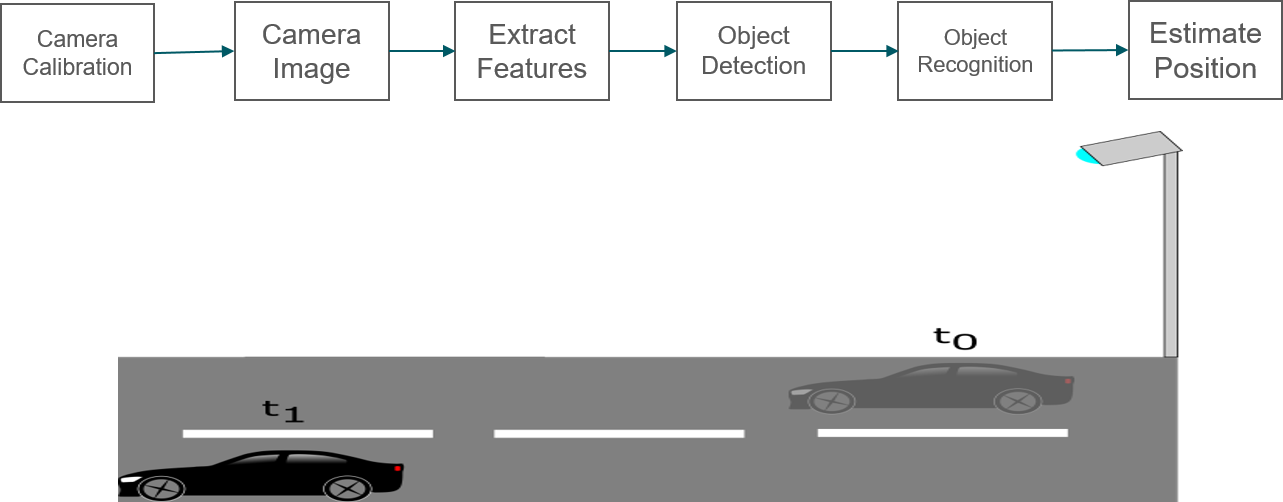
\includegraphics[width=\textwidth]{imagens/proposal1.png}
\caption{Proposal using only one camera with object calibration}
\label{fig:proposal1}
\end{figure}

\subsection{Camera Calibration}

This task is necessary to reduce the distortion of the camera. The camera used on the tasks has a noise, for this approach is recommended to perform this step. Following this requirement, a script in Python language with the OpenCV library based in \cite{zhu2020camera} was developed. Furthermore, with calibration, also it is possible to determine the relationship between the camera's natural units (pixels) and the real-world units (for example, millimeters).

Using the intrinsic parameters of the camera, as in (\ref{eq:calibration}), and one point is projected on the image plane. 


\begin{equation}
    \label{eq:calibration}
    \begin{bmatrix}
        u'
        \\v' 
        \\ z' 
        
        \end{bmatrix} = P \begin{bmatrix}
        X_w\\
        Y_w 
        \\ Z_w
        \\ 1
        
        \end{bmatrix}
\end{equation}

The 3D point ($X_w, Y_w, Z_w$) in the world coordinates to its projection ($u, v$) in the image coordinates. The calibration algorithm calculates the camera matrix using the extrinsic and intrinsic parameters. The extrinsic parameters represent a rigid transformation from 3-D world coordinate system to the 3-D camera’s coordinate system. The intrinsic parameters represent a projective transformation from the 3-D camera’s coordinates into the 2-D image coordinates. Figure \ref{fig:block_extrinsinc} is shown the block diagram where explains the problematic to convert a pixel to the real world. 


\begin{figure}[H]
\centering
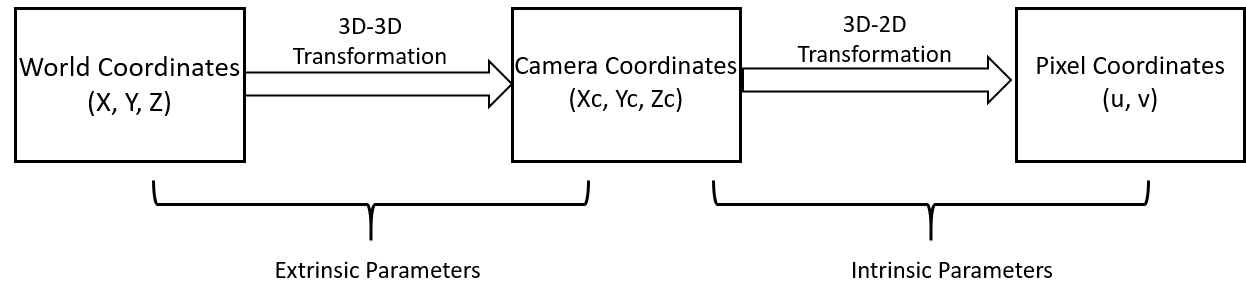
\includegraphics[scale=0.8]{imagens/block_parameters.png}
\caption{Block diagrams of a projection}
\label{fig:block_extrinsinc}
\end{figure}





In (\ref{eq:points}), $\mathbf{P}$ is a 3x4 projection matrix combined of two different parts, the intrinsic parameters of the camera ($\mathbf{K}$) and the extrinsic matrix ($[\mathbf{R}|t]$) that is based on the combination of 3x3 rotation matrix $\mathbf{R}$ and 3x1 translation $t$ vector \cite{kaehler2016learning}. 

\begin{equation}
    \label{eq:points}
    P = \overbrace{\hbox{\boldsymbol{K}}}^{\hbox{Intrinsic Matrix}} \cdot \overbrace{\hbox{[\boldsymbol{R}|t]}}^{\hbox{Extrinsic Matrix}}
\end{equation}

The intrinsic matrix ($\mathbf{K}$) is an upper triangular matrix as shown in (\ref{eq:intrisic}). 

\begin{equation}
    \label{eq:intrisic}
\textbf{K} = \begin{bmatrix}
    f_x & \gamma  & c_x\\ 
    0 & f_y & c_y\\ 
    0 & 0 & 1
    \end{bmatrix}
\end{equation}

where, $f_x, f_y$ are the $x$ and $y$ focal lengths, $c_x, c_y$ are the $x$ and $y$ coordinates of the center in the image plane, $\gamma$ is the skew between the axes, in this master's thesis, was defined equal to $0$.  

The Extrinsic Matrix is shown in (\ref{eq:ext}). The extrinsic matrix takes the form of a rigid transformation matrix: a 3x3 rotation matrix in the left-block, and 3x1 translation column-vector in the right. The camera's extrinsic matrix describes the camera's location in the world, and what direction it is pointing. 

\begin{equation}
    \label{eq:ext}
    [ R \, |\, \boldsymbol{t}] = 
\left[ \begin{array}{ccc|c} 
r_{1,1} & r_{1,2} & r_{1,3} & t_1 \\
r_{2,1} & r_{2,2} & r_{2,3} & t_2 \\
r_{3,1} & r_{3,2} & r_{3,3} & t_3 \\
\end{array} \right]
\end{equation}

\subsection{Camera Image}

The image camera model depicted in Figure \ref{fig:image_formation} describes the mathematical relationship between the coordinates of a point in 3-dimension space and its projection onto
the image plane of a camera, where this aperture is described as a point, and no lenses are used to focus light. The model can only be used as a first-order approximation of the mapping from a 3D scene to a 2D image \cite{forsyth2002computer}.




\begin{figure}[H]
\centering
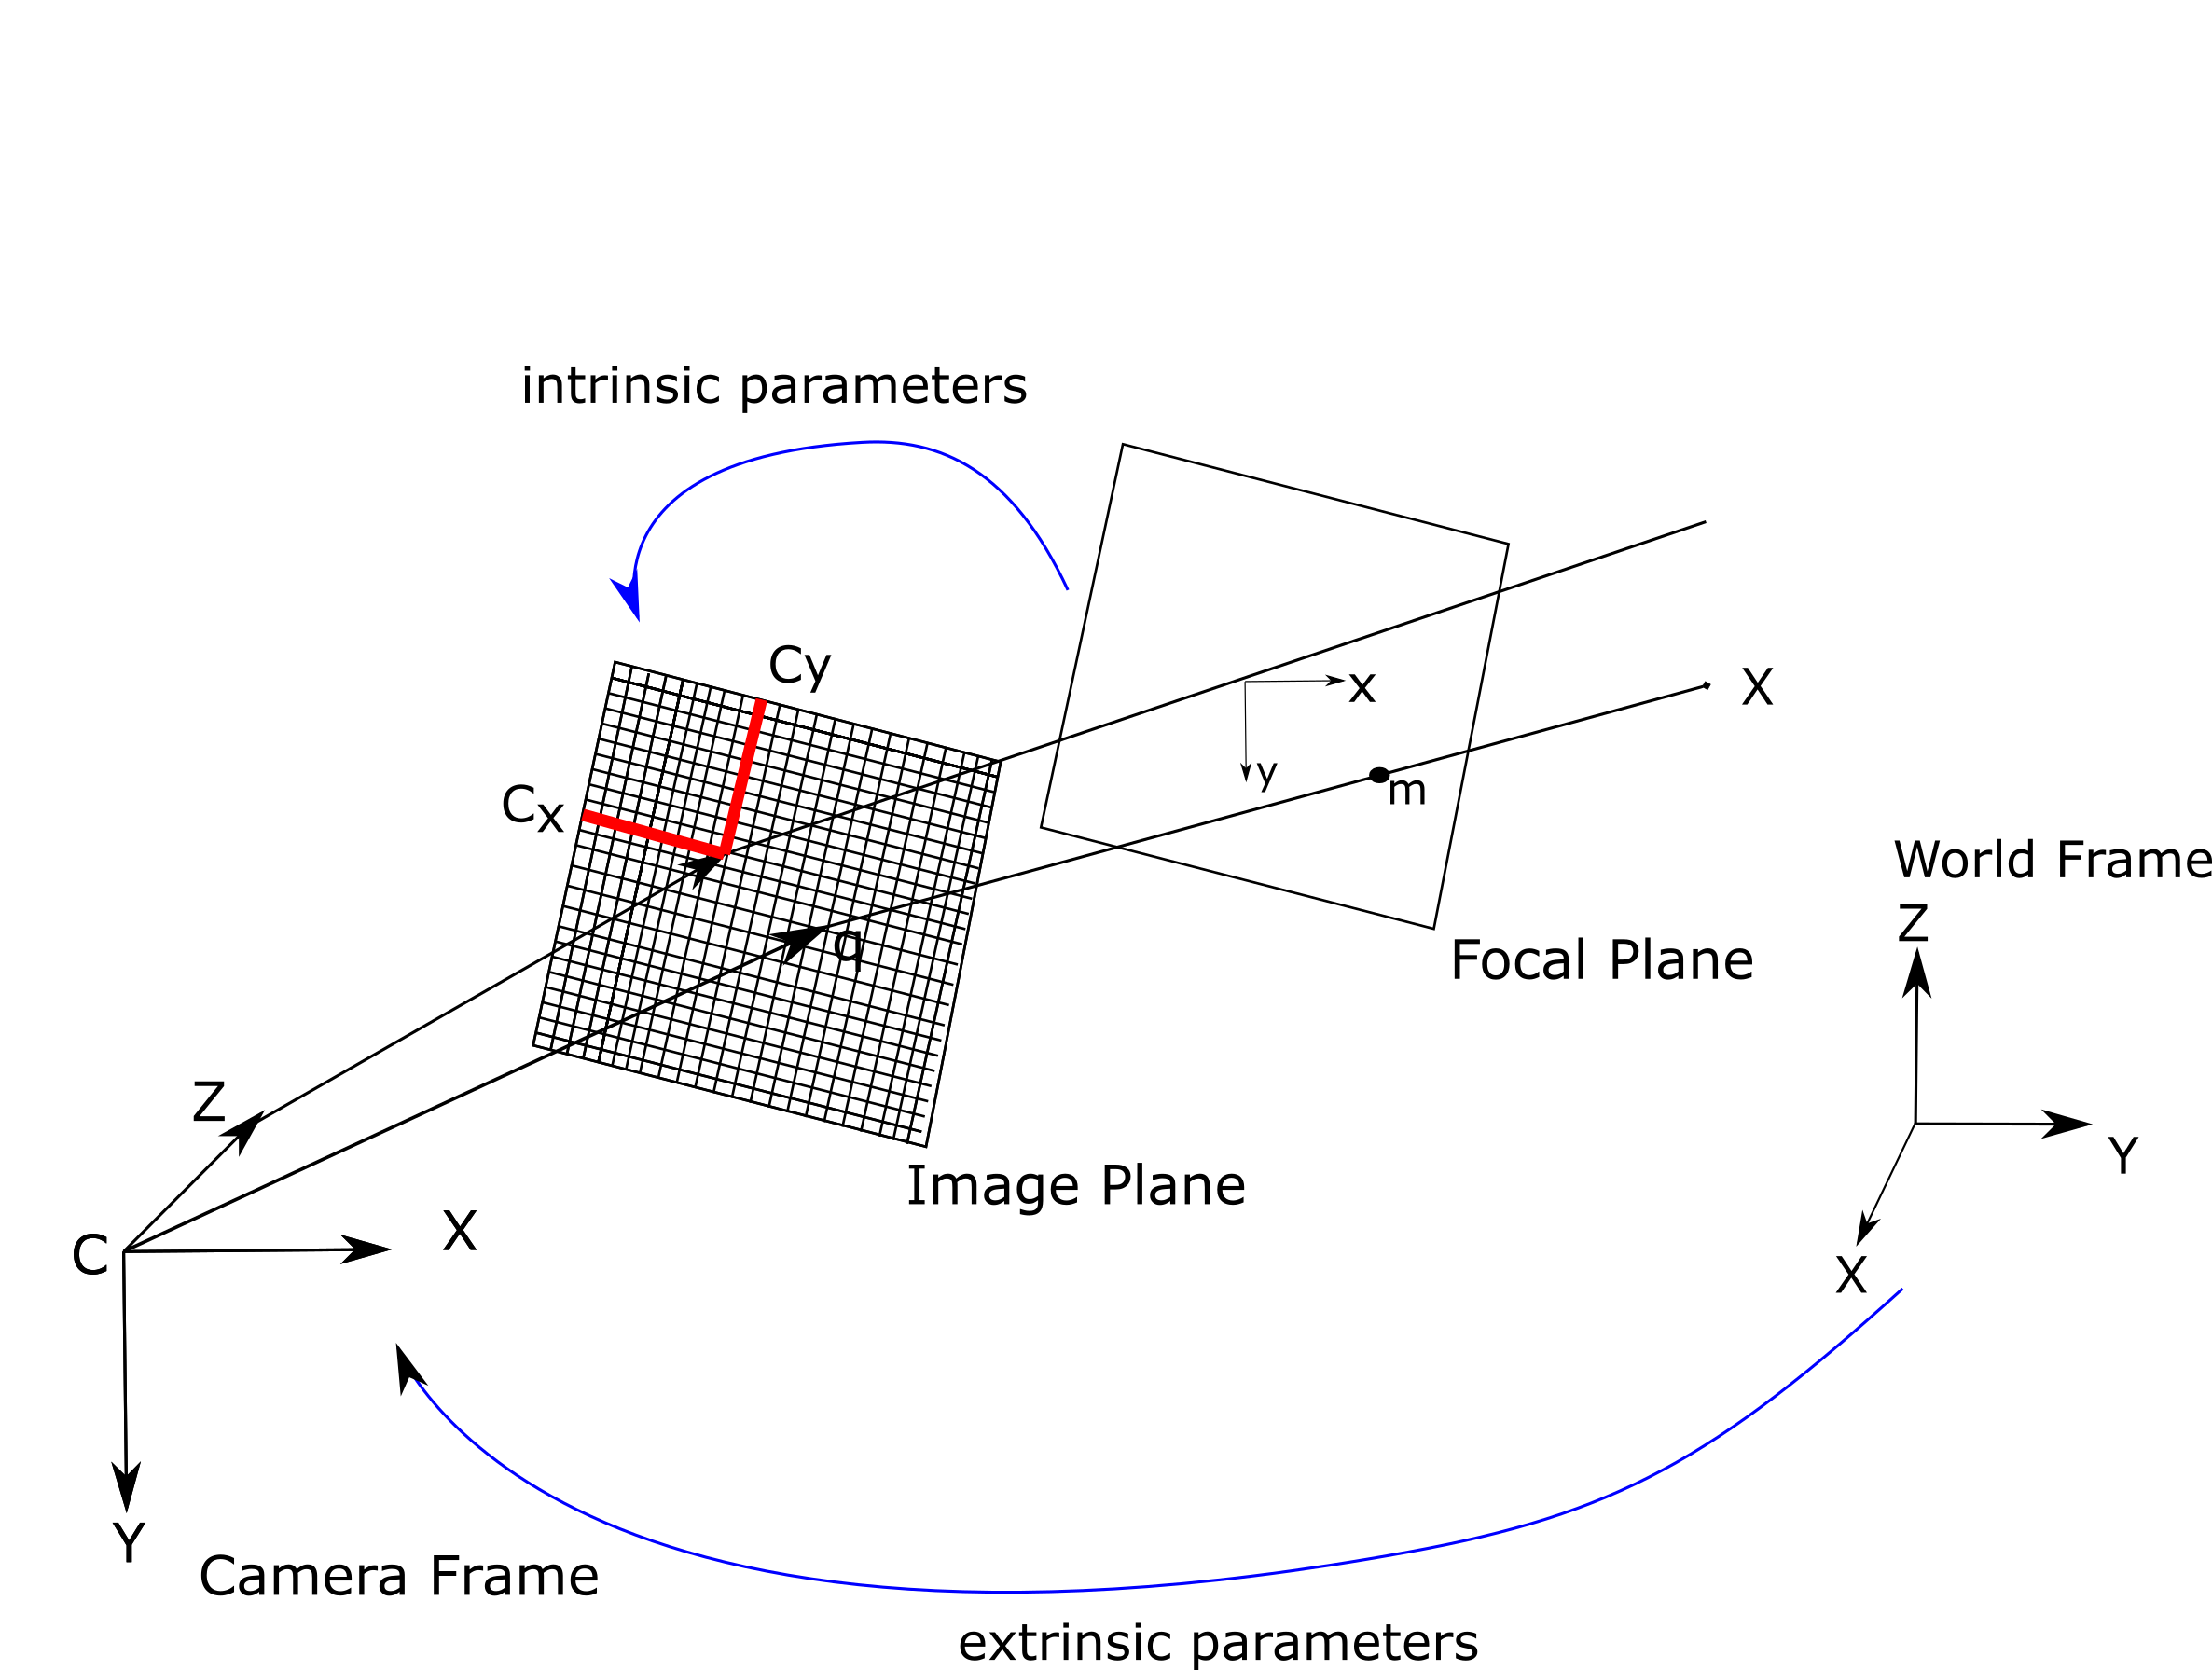
\includegraphics[width=\textwidth]{imagens/image_formation.png}
\caption{The camera model for image formation based on some metrics and known parameters}
\label{fig:image_formation}
\end{figure}

\subsection{Features Extraction}

When it is necessary to work with variables that contain many contents, there is a necessity to improve this work and reduce the computer bottleneck during the process. In machine learning (ML), some variables are independents or some features on which the final output is done. Moreover, in other cases, that number of these features increases it and reduces the ability to visualize it. 

For example, the image resolution of the collected data for the ML algorithm's training is $1392$ pixels in height and $512$ pixels in width, for the total $712,704$ pixels in total. Each pixel has a single pixel-value associated with it, indicating the darkness or lightness of that pixel. The numbers are between $0$ and $255$, along this premise is necessary to determine which objects the image contains.

The task was performed by feature extraction, which creates new features from existing features, giving us more information and fewer redundancies \cite{wang2019data}.

A mathematical tool called Principal Component Analysis (PCA) was used in this step, and the PCA is used to decompose a multivariate dataset in a set of successive orthogonal components that explain a maximum amount of the variance \cite{pedregosa2011scikit}. Figure \ref{fig:pca_step1} is shown how the technique works. The data is decomposed into a perpendicular vector where the information is unrolled. Besides, with more variance means more information regarding data.

\begin{figure}[H]
\centering
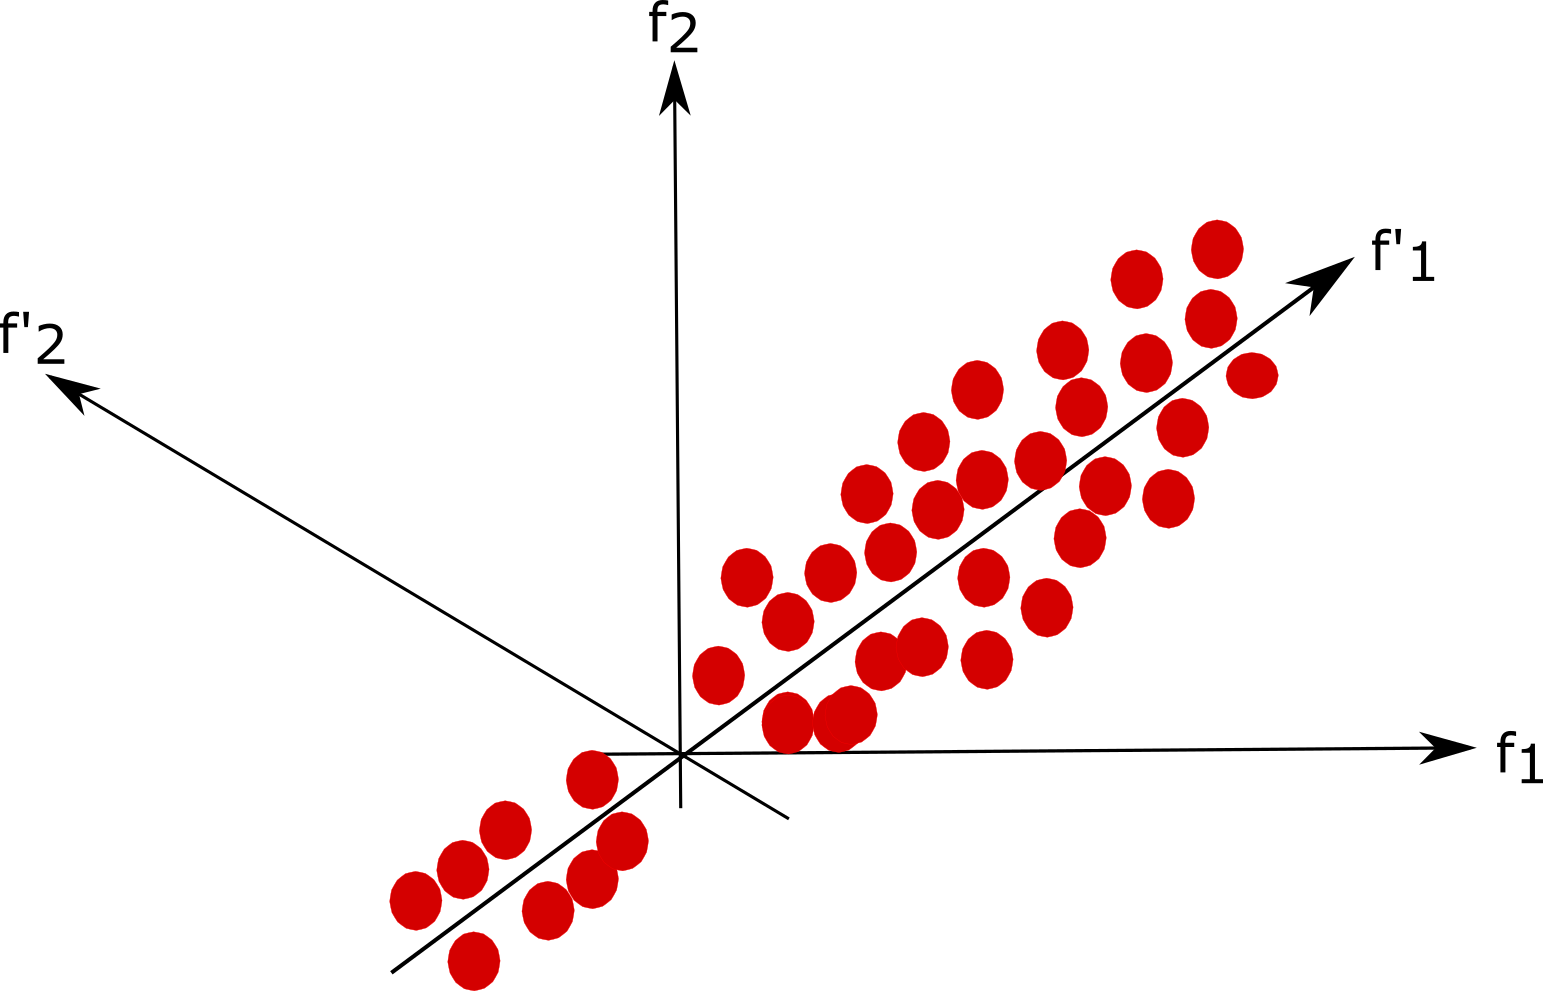
\includegraphics[scale=0.7]{imagens/pca1.png}
\caption{Maximum variance in $f_1'$, where the red circles mean the data points of the data set, $f_1$ is the feature 1 on x-axis, $f_2$ is the feature 2 on y-axis}
\label{fig:pca_step1}
\end{figure}


Based on Figure \ref{fig:pca_step2}, is necessary to find a direction $f_i$ such as the variance of $x_i's$ project on $f_i's$ has the maximum value. Also, it is necessary to rotate the previous axis to find $f_i' s$, and finally, drop $f_2$

\begin{figure}[H]
\centering
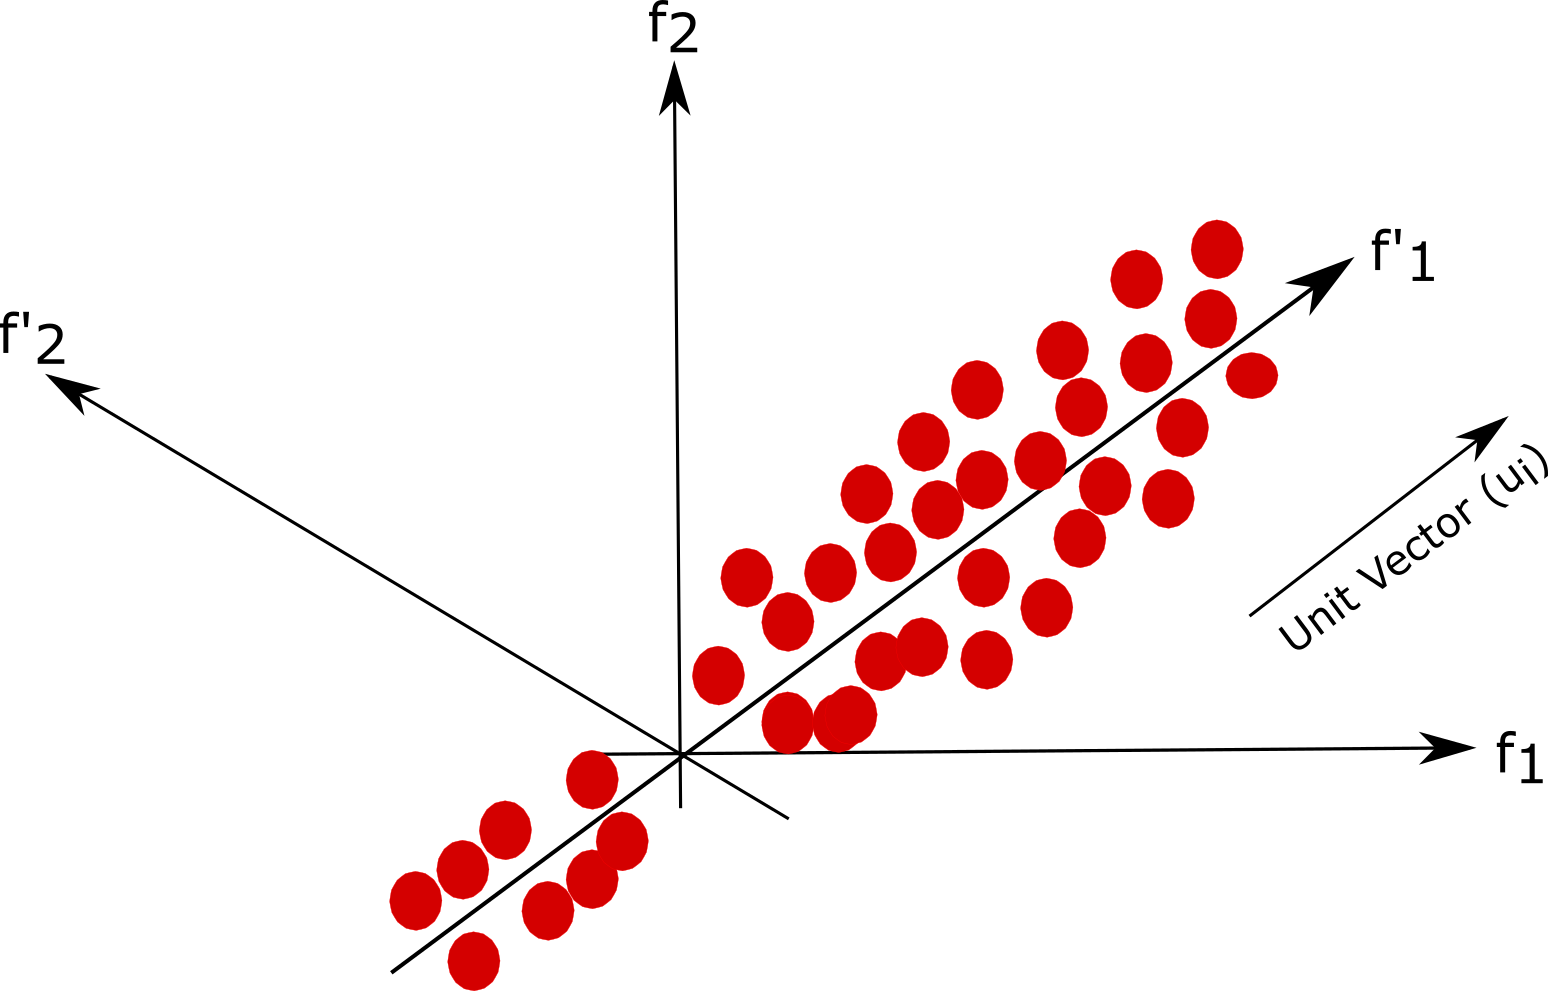
\includegraphics[scale=0.7]{imagens/pca2.png}
\caption{Unit vector direction of maximum variance}
\label{fig:pca_step2}
\end{figure}

To find the direction of $ f_i's $, which has the maximum variance, thus, unit vector in the direction of maximum variance = $U_i$, in (\ref{eq:eq_pca}) is described how to compute this distance. 


\begin{subequations}
\begin{equation}
    \label{eq:eq_pca}
    x_i' = \textnormal{Projection of} ~ x_i ~\textnormal{on unit vector} ~u_i
\end{equation}
  
\begin{equation}
  = u_i^Tx_i
\end{equation}

\begin{equation}
    \overline{x_i'} = u_i^T\cdot\underbrace{\overline{x}_i}_{Mean ~ Vector}
\end{equation}
\begin{equation}\label{step_pca}
    var\left \{ u^Tx_i \right \}^n_{i=1} = \frac{1}{n}\sum_{i=1}^{n}\left ( u_i^Tx_i - \underbrace{u_i^T\overline{x}_i}_{Mean~\overline{x}_i} \right )^2
\end{equation}

\end{subequations}

In (\ref{step_pca}) is possible to find out the $u_i$ which gives the maximum variance. Further, this problem can be defined as distance minimization \cite{liu2004distance}. 

In Figure \ref{fig:pca_step3} the vector which gives the minimum distance $(d_1,d_1, \cdots)$ when $x_i's$ are projected on $u_i$. 

\begin{figure}[H]
\centering
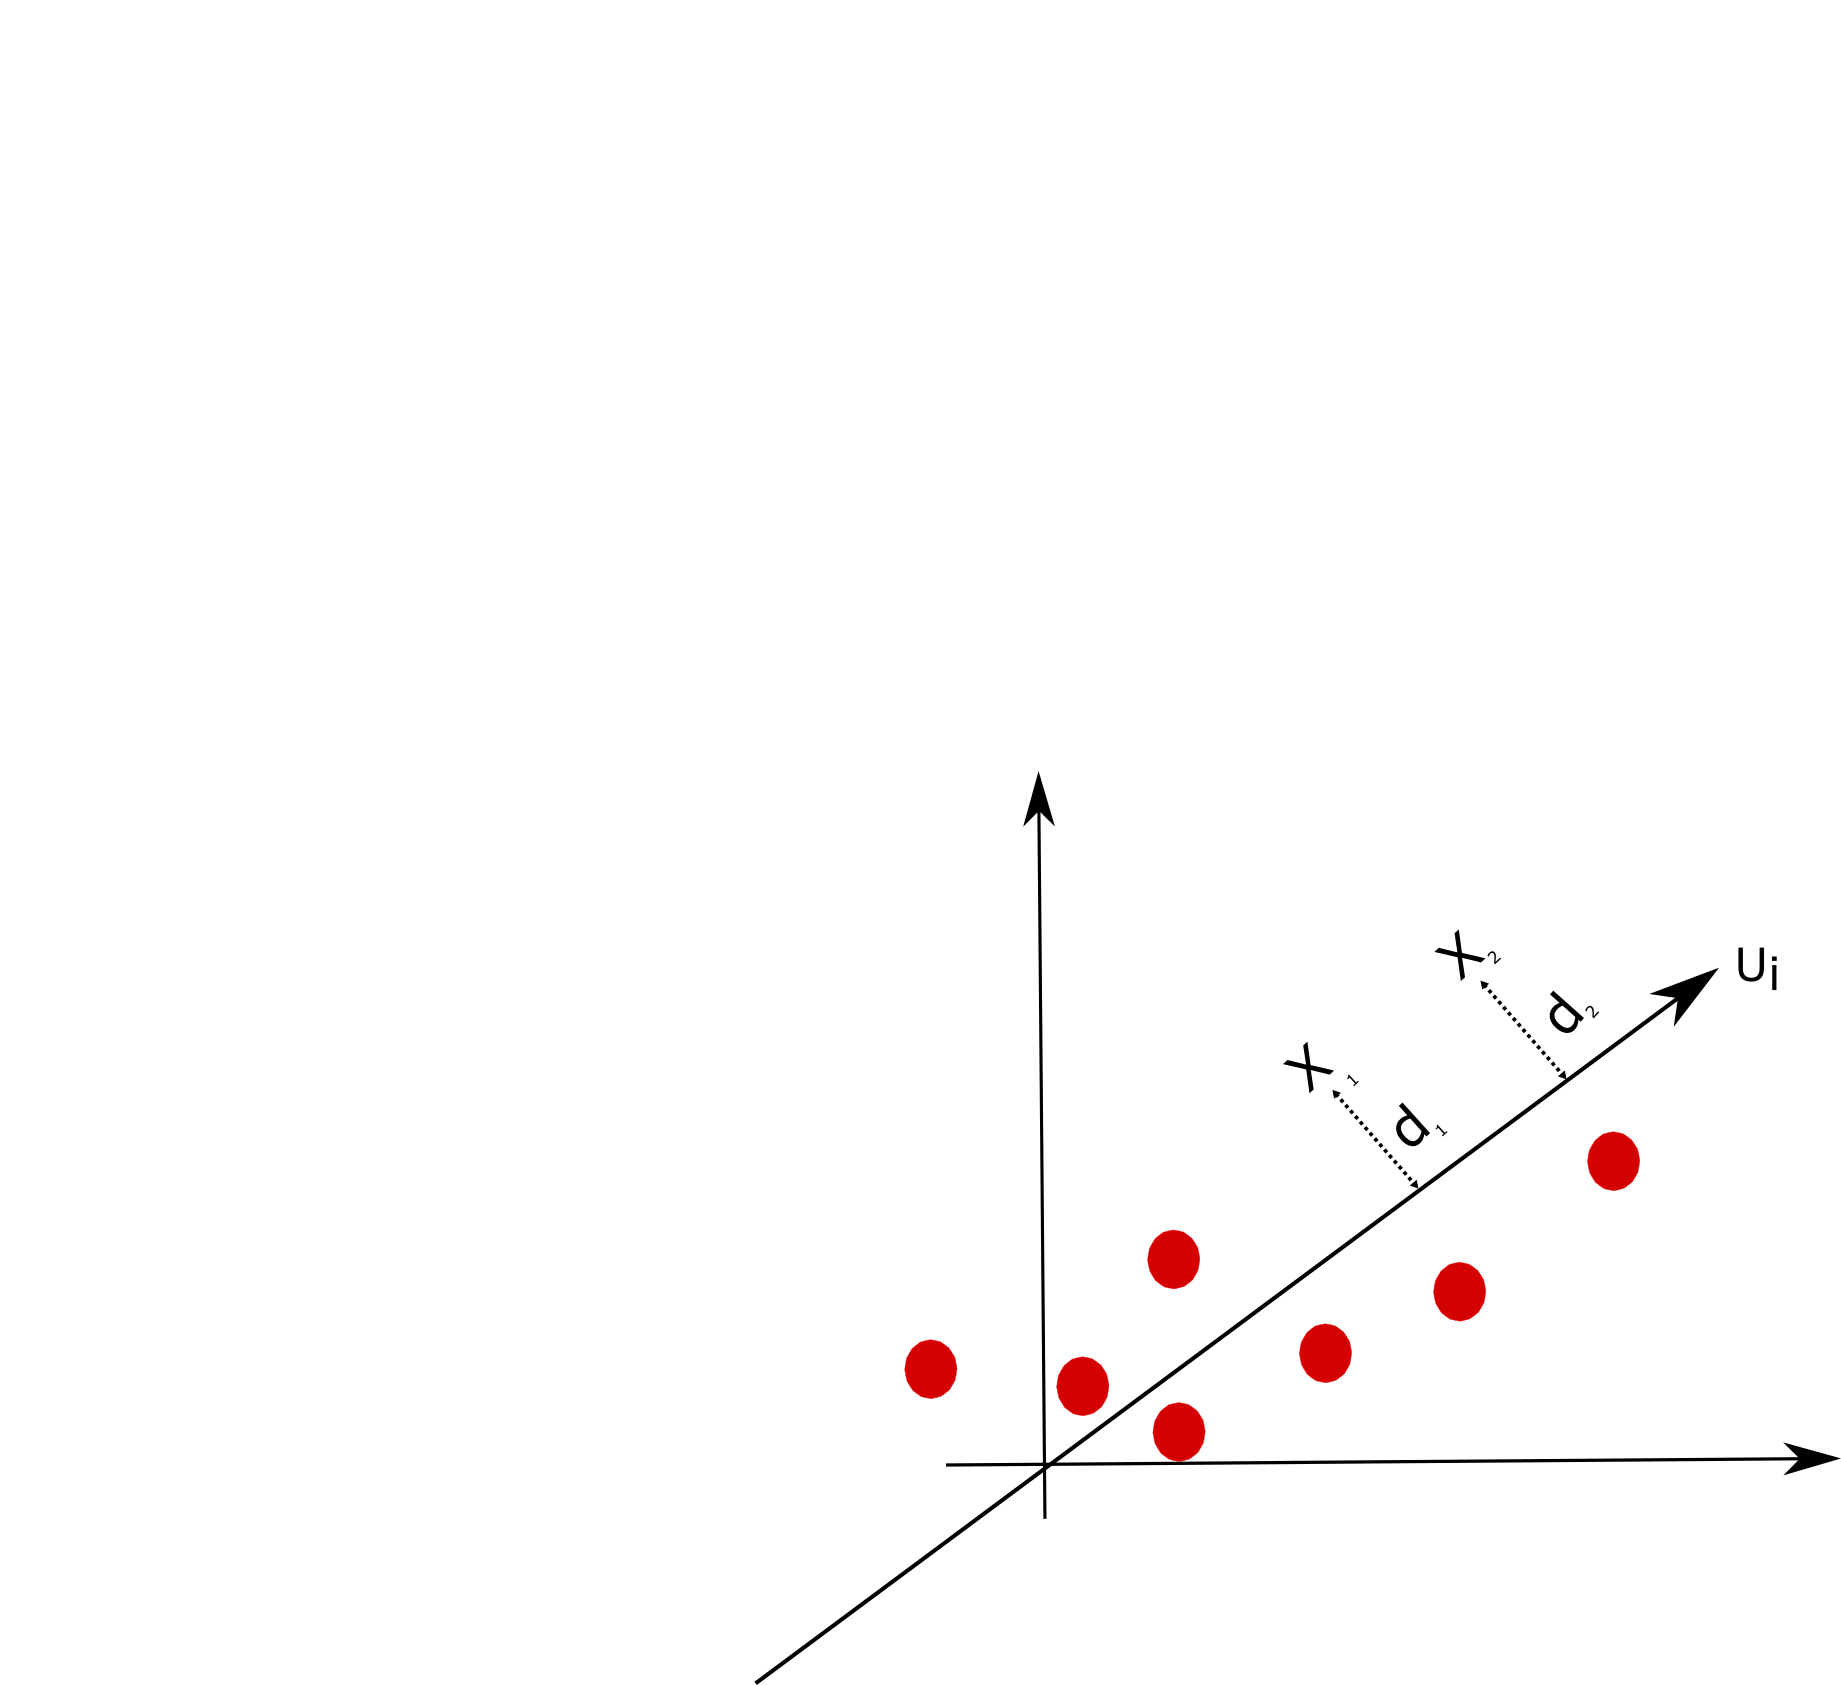
\includegraphics[scale=0.7]{imagens/pca3.png}
\caption{Distance minimization PCA}
\label{fig:pca_step3}
\end{figure}

In (\ref{eq:pca_4}), the equation finds the vector $u_i$, which gives the minimum distance. 

\begin{subequations}
    \label{eq:pca_4}
    \begin{equation}
        d_i^2 = \left \| x_i \right \|^2 - \left ( u^Tx_i \right )^2
    \end{equation}
    \begin{equation}
        = \left ( x^Tx_i \right ) - (u^Tx_i)^2
    \end{equation}
    \begin{equation}
        min_{u_i} \sum_{i=1}^{n}\left ( x_i^Tx_i - \left ( u^Tx_i \right )^2 \right )
    \end{equation}
\end{subequations}

Calculation of Eigenvalues and Eigenvectors give the solution to the above Equations. 

where the matrix $\mathbf{X}$ in (\ref{eq:matrix}) is the matrix of the data points with the shape $(n x d)$

\begin{equation}\label{eq:matrix}
    \mathbf{X} = \begin{bmatrix} 
    a_{11} & a_{12} & \dots \\
    \vdots & \ddots & \\
    a_{K1} &        & a_{KK} 
    \end{bmatrix}
\end{equation}

The square symmetric matrix is defined as $S_{dxd} = X^T_{dxn}X_{nxd}$ \cite{Halko_2011}. 

Based on the approach of \cite{cambridge2009introduction}, in (\ref{eq:svd}) is defined the solution equation.

\begin{equation}
    \label{eq:svd}
    \lambda_i V_{i_{dx1}} = S_{dxd}V_{i_{dx1}}
\end{equation}

where $\lambda$ is the scalar eigenvalues, $S$ is the co-variance matrix, $V$ is the vector - eigenvector, and $d$ is the dimension.

The steps to find the Eigenvector: 

\begin{enumerate}
    \item Do the column standardization of $\mathbf{X}$
    \item compute the co-variance Matrix: $S = X^TX$
    \item $\lambda = $ Eigen Value and $V$ = Eigen Vector
    \item $\lambda V = SV$
\end{enumerate}

To brief these steps is necessary to assume the more variability in a particular direction correlates with explaining the dependent variable's behavior. Theoretically, it is needed to apply the PCA to remove the sample's noise and keep only the necessary things to detect.


\subsection{Object Detection and Object Recognition} 

This task is based on the paper \cite{redmon2016you}, where You Only Look Once (YOLO) version 3 is used as an object detector and uses the features after the pre-processing as input the deep convolutional neural network in Figure \ref{fig:yolo_arc}.  

\begin{figure}[H]
\centering
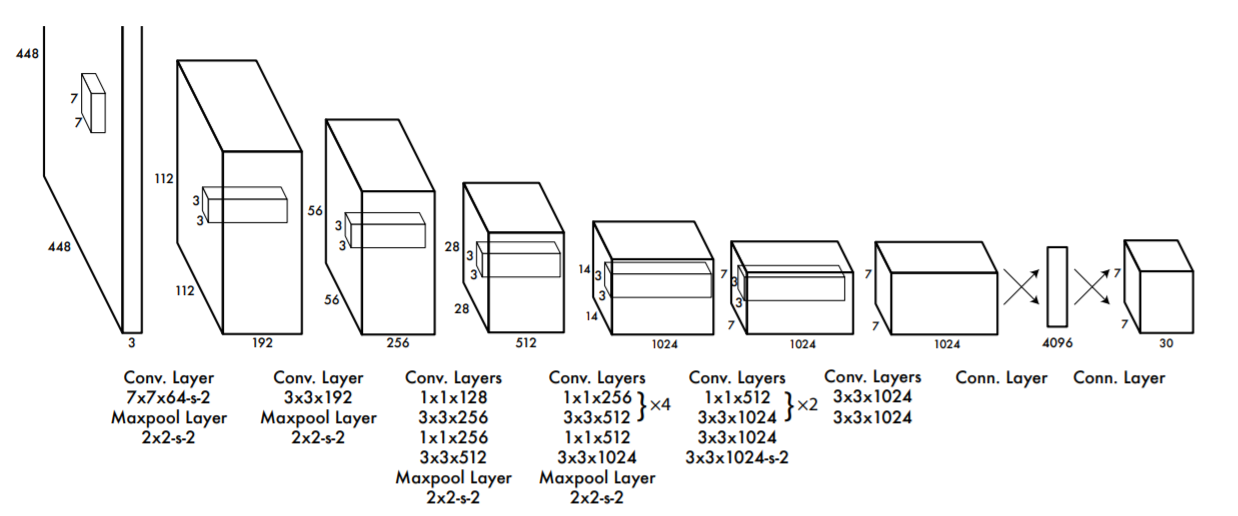
\includegraphics[width=\textwidth]{imagens/yolo.png}
\caption{YOLO Architecture: Simultaneously predicts bounding boxes and class probabilities for these boxes \cite{redmon2016you}}
\label{fig:yolo_arc}
\end{figure}

This architecture makes use of only convolutional neural networks. This topic has already been detailed in Subsection \ref{sec:cnn} and makes it in a fully convolutional network (FCN). Yolo has $75$ convolutional layers, with skip connections and upsampling layers.  





In the YOLO environment, the algorithm divides the input image into a $ZxZ$ grid. Each grid of this frame predicts only one object, as shown in Figure \ref{fig:yolo_flow}. Along, YOLO uses $7x7$ grids ($ZxZ$), two boundary boxes (B), and 20 classes (C). So, the tensor of the YOLO prediction has a shape of $(Z, Z, Bx5+20) = (7,7,30)$


\begin{figure}[H]
\centering
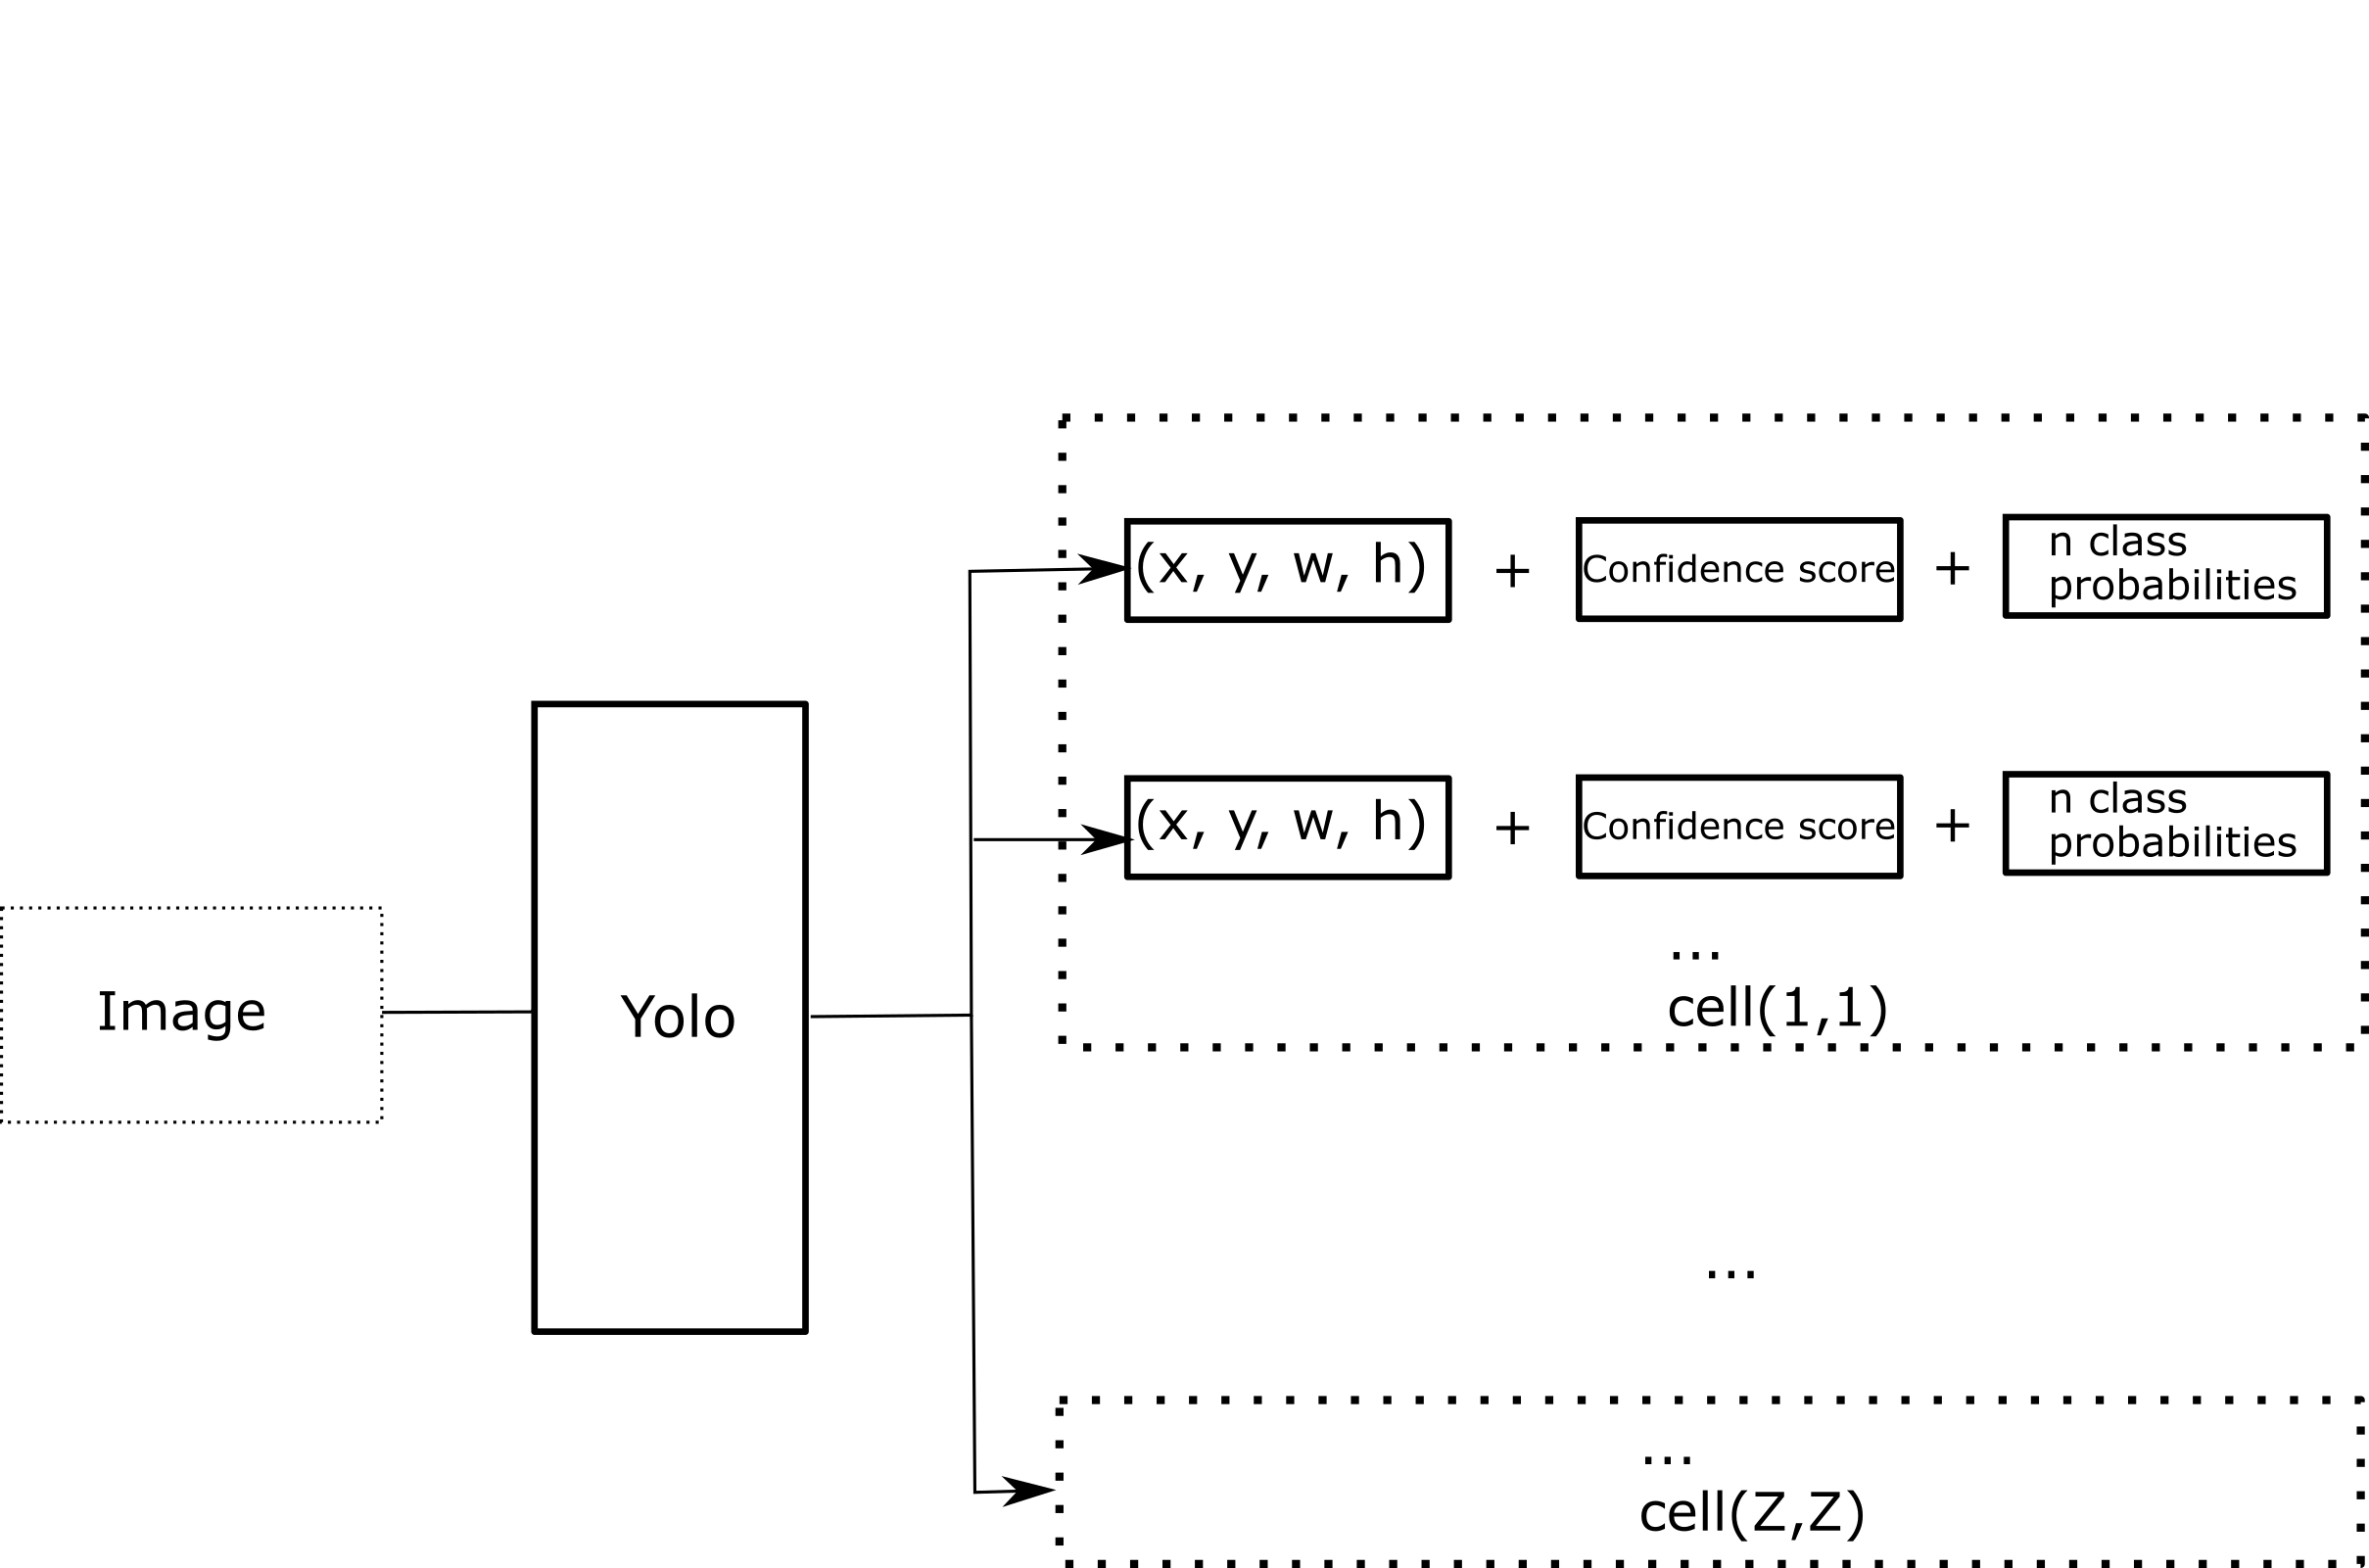
\includegraphics[scale=0.7]{imagens/yolo_flow.png}
\caption{Yolo makes ZxZ predictions with B boundaries boxes}
\label{fig:yolo_flow}
\end{figure}

The object detection is based on the boundary box approach, and each box has five known elements (x, y, w, h) and a box confidence score. This score means how likely the box contains an object. It uses CNN to reduce the spatial dimension; after that, it performs a linear regression using two fully connected layers to make the predictions; this approach considers only predictions over 0.5. It is defined in Table \ref{eq:prob_yolo}. 


\begin{table}[H]
\centering
\caption{The Yolo's predicts equations}
\begin{tabular}{l|l} 
\toprule
Description~                   & Equation                                                                 \\
box confidence score           & $P_r(object).IoU$                                                     \\
conditional class probability~ & $P_r(class_i|object)$                                       \\
class confidence score         & $P_r(class_i).IoU$                                                   \\
class confidence score         & box confidence score $\cdot$ conditional class probability  \\
\bottomrule
\end{tabular}
\label{eq:prob_yolo}
\end{table}

where in Table \ref{eq:prob_yolo},$P_r(object)$ is the probability the box contains an object.
$IoU$ is the intersection over the union between the predicted box and the ground truth.
$P_r(class_i|object)$ is the probability the object belongs to $class_i$ given an object is presence.
$P_r(class_i)$ is the probability the object belongs to $class_i$.

The bounding boxes concept is defined in \cite{redmon2017yolo9000}, and in the many problems as in the autonomous driving domain, the most common detection will be pedestrians and cars at different distances \cite{ess2010object}.  It is necessary to apply the clusterization approach. In this case, it is defined by K-means with $K=5$. Since the algorithm is working with many kinds of bounding boxes, it is not possible to use the regular spatial distance to measure the data point distances, that is the reason to use $IoU$. Based on the length of the cluster called as the anchor, in this solution will predict five parameters ($t_x, t_y, t_w, t_h,$ and $t_o$) combined with the sigma function to reduce the offset range as is already defined in (\ref{eq:bound}) and it is detailed graphically in Figure \ref{fig:anchor}.


    
    \begin{equation}
    \label{eq:bound}
    \begin{aligned}
        b_x = \sigma(t_x) + c_x \\
        b_y = \sigma(t_y) + c_y \\
        b_w = p_we^{t_w} \\
        b_h = p_he^{t_h} \\
        P_r(object)\cdot IoU(b,object) = \sigma(t_o)
    \end{aligned}
    \end{equation}

where, $t_x, t_y, t_w, t_h$ are the predictions made by the algorithm. 
$c_x, c_y$ are the top left corner of the grid cell of the anchor.
$p_w, p_h$ are the width and height of the anchor. 
The image width and height normalize $ c_x, c_y$. 
$b_x, b_y, b_w, b_h$ are the predicted boundary box. 
$\sigma(t_i)$ is the box confidence score.

\begin{figure}[H]
\centering
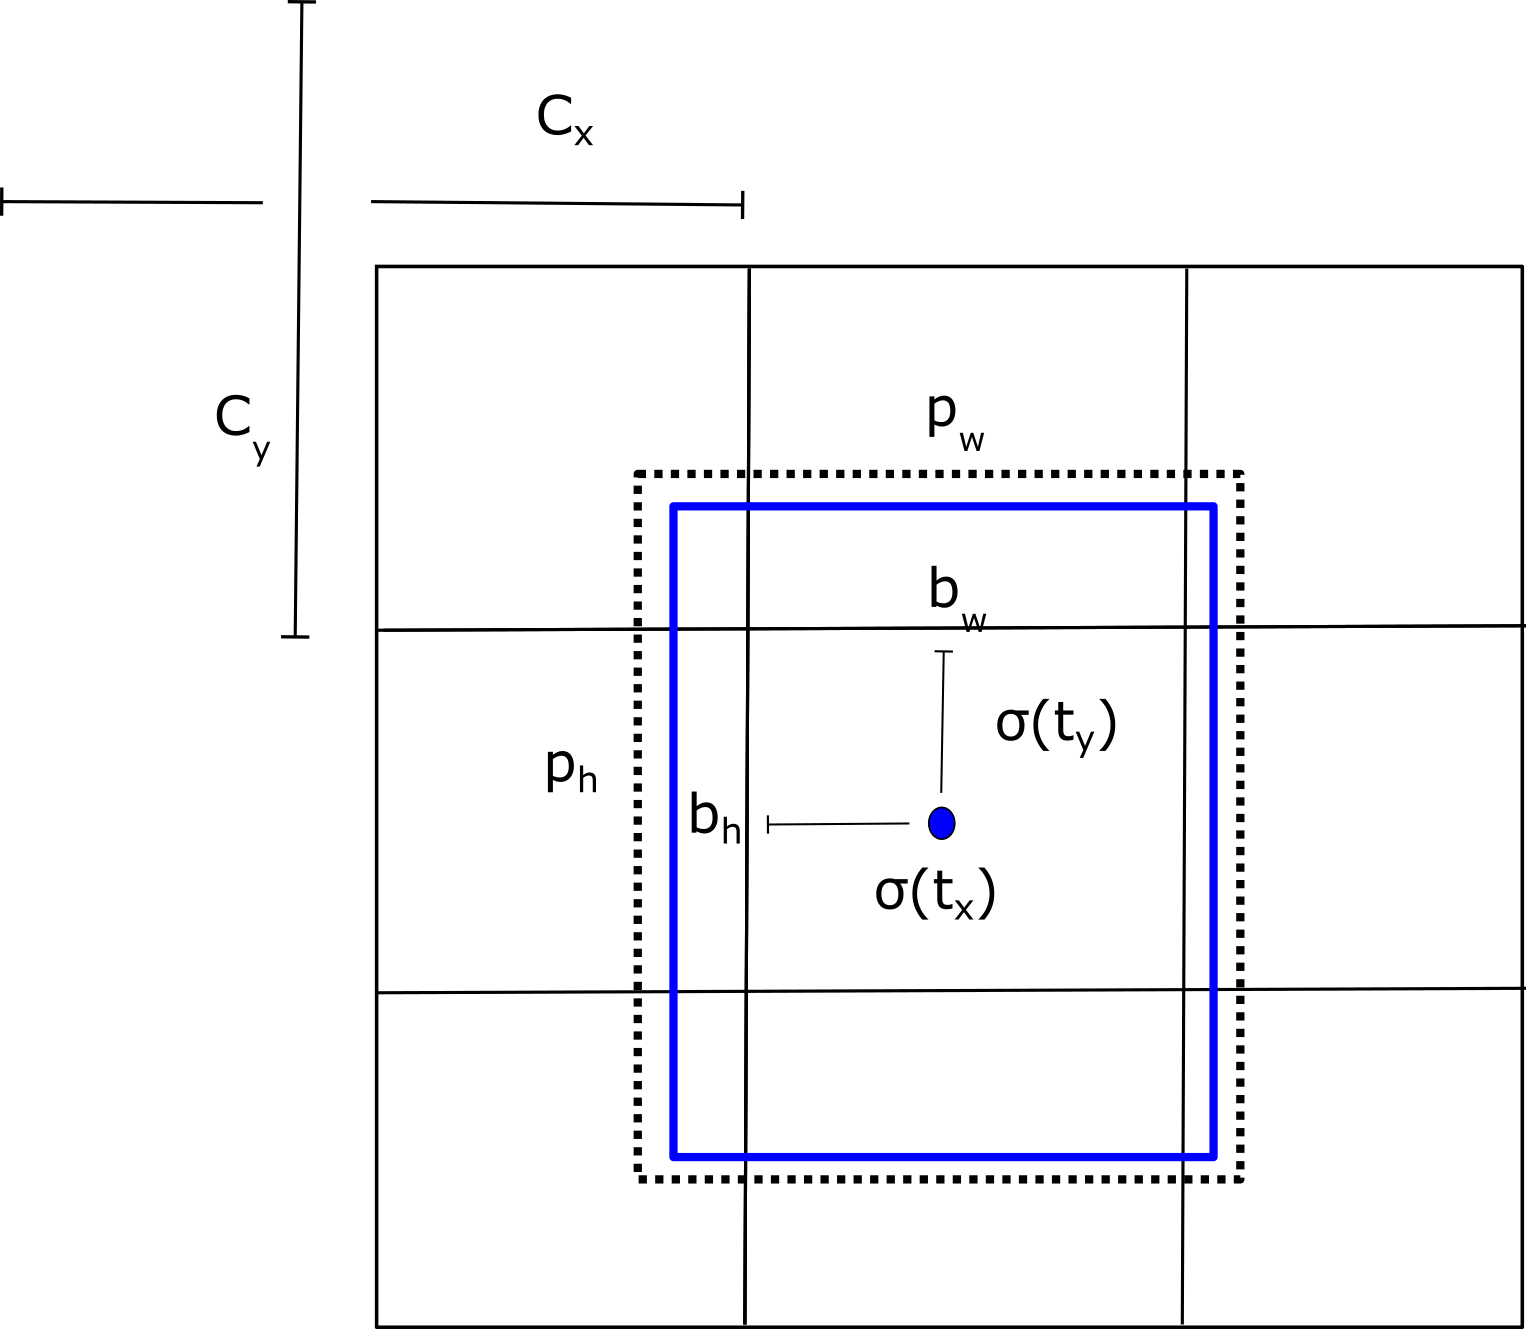
\includegraphics[scale=0.5]{imagens/anchor.png}
\caption{Prediction of the width and height of the box as offsets from clusters centroids based on \cite{redmon2017yolo9000}}
\label{fig:anchor}
\end{figure}

As already defined, the proposed solution predicts multiple bounding boxes per grid cell. Thus, it is necessary to compute the loss for the true positive, to reduce the error. Hence the object is to be faster, not accurate. On the other hand, each cell will be looked at time and use, and it will be used the highest IoU. The loss function is composed by classification loss in (\ref{eq:classification_loss}), the localization loss in (\ref{eq:localization_loss}), the confidence loss (\ref{eq:confidence_loss}), and the loss function is (\ref{eq:loss}). 

If the object is located on the frame, the classification loss will perform the squared error at each cell on the conditional probability for each class: 

\begin{equation}
\label{eq:classification_loss}
    \sum_{i=0}^{s^2}1^{obj}_i \sum_{c\in~classes} \left ( p_i\left ( c \right )-\hat{p}_i\left ( c \right )\right )^2
\end{equation}

where $1^{obj}_i$ is the Boolean that controls if has an object or not, $\hat{p}_i\left ( c \right )$ denotes the conditional probability for each class in the cell.

The localization loss is necessary to take care of the measurement errors regarding the locations and the boxes' sizes. The goal is not to define the absolute weight errors in large boxes and small boxes. It predicts the square root of the bounding box width and height instead of the width and height. 

\begin{equation}
\label{eq:localization_loss}
\begin{aligned}
    \lambda_{coord}\sum_{i=0}^{s^2}\sum_{j=0}^{B}1^{obj}_i_j\left [ \left ( x_i - \hat{x_i} \right )^2  + (y_i-\hat{y_i})^2 \right ] \\ 
    + \lambda_{coord}\sum_{i=0}^{s^2}\sum_{j=0}^{B}1^{obj}_i_j\left [ \left ( w_i - \hat{w_i} \right )^2  + (h_i-\hat{h_i})^2 \right ] 
    \end{aligned}
\end{equation}

where $1_{ij}^{obj} = 1$ if the boundary box in the cell is responsible for detecting the object, otherwise is 0. $\lambda_{coord}$ increases the weight for the loss in the boundary boxes coordinates, with this variable is possible to put more emphasis on the accuracy, so it is multiplied by the loss, the default value for this work is 5. 

The confidence loss is used to measure the box's objectness because a significant part of the boxes does not have any detector inside, and with this, an imbalance issue is noted to avoid this object is necessary to compute this loss. 

\begin{equation}
    \label{eq:confidence_loss}
    \lambda_{noobj}\sum_{i=0}^{s^2}\sum_{j=0}^{B}1^{noobj}_{ij}\left ( C_i - \hat{C}_i \right )^2
\end{equation}

where $1^{noobj}_i$ is the complement of $1^{obj}_i$, $\hat{C}_i$ is the box confidence score of the box $j$ in cell $i$, and $\lambda_{noobj}$ takes care of the weights decrease the loss when the background is detected in this work the used value for this variable is $0.5$. 

The final loss is computed through the addition of previous losses, in (\ref{eq:loss}) is defined as the actual loss to reduce the errors in the object detection.

\begin{equation}
\label{eq:loss}
\begin{aligned}
    \lambda_{coord}\sum_{i=0}^{s^2}\sum_{j=0}^{B}1^{obj}_i_j\left [ \left ( x_i - \hat{x_i} \right )^2  + (y_i-\hat{y_i})^2 \right ] \\ 
    + \lambda_{coord}\sum_{i=0}^{s^2}\sum_{j=0}^{B}1^{obj}_i_j\left [ \left ( w_i - \hat{w_i} \right )^2  + (h_i-\hat{h_i})^2 \right ] \\
+    \sum_{i=0}^{s^2}\sum_{j=0}^{B}1^{noobj}_{ij}\left ( C_i - \hat{C}_i \right )^2\\
+  \lambda_{noobj}\sum_{i=0}^{s^2}\sum_{j=0}^{B}1^{noobj}_{ij}\left ( C_i - \hat{C}_i \right )^2\\
+     \sum_{i=0}^{s^2}1^{obj}_i \sum_{c\in~classes} \left ( p_i\left ( c \right )-\hat{p}_i\left ( c \right )\right )^2
    \end{aligned}
\end{equation}

After object detection, it is necessary to perform the object classification, where each box predicts the classes the bounding box, so it is recommended to use multilabel classification. The difference in this work is to use the softmax function in the output of the categories. The data used in this training is labeled, and it was collected from Open Image Dataset \cite{krasin2017openimages}, and this classification was performed over the Darknet neural network \cite{redmon2013darknet}.

\subsection{Distance Estimation}

This approach uses the object detector's outputs for the distance estimation, where $4$ variables are predicted, which are $(x, y, w, h)$. This work variables $x,y$ are used to adjust the boundary box and $w, h$ are used in Figure \ref{fig:yolo_flow} to measure the distance of the object. These variables will variate according to the distance of the camera.  In \cite{cao2013circle} the image will be refracted in the lens, and with this is possible to deduce a relationship between the known parameters: focal length $(f)$, the distance of the object from the lens $(d)$, the distance of the refracted image from the lens $(D)$. In Figure \ref{fig:distance} is shown how the distance measurer works. 


\begin{figure}[H]
\centering
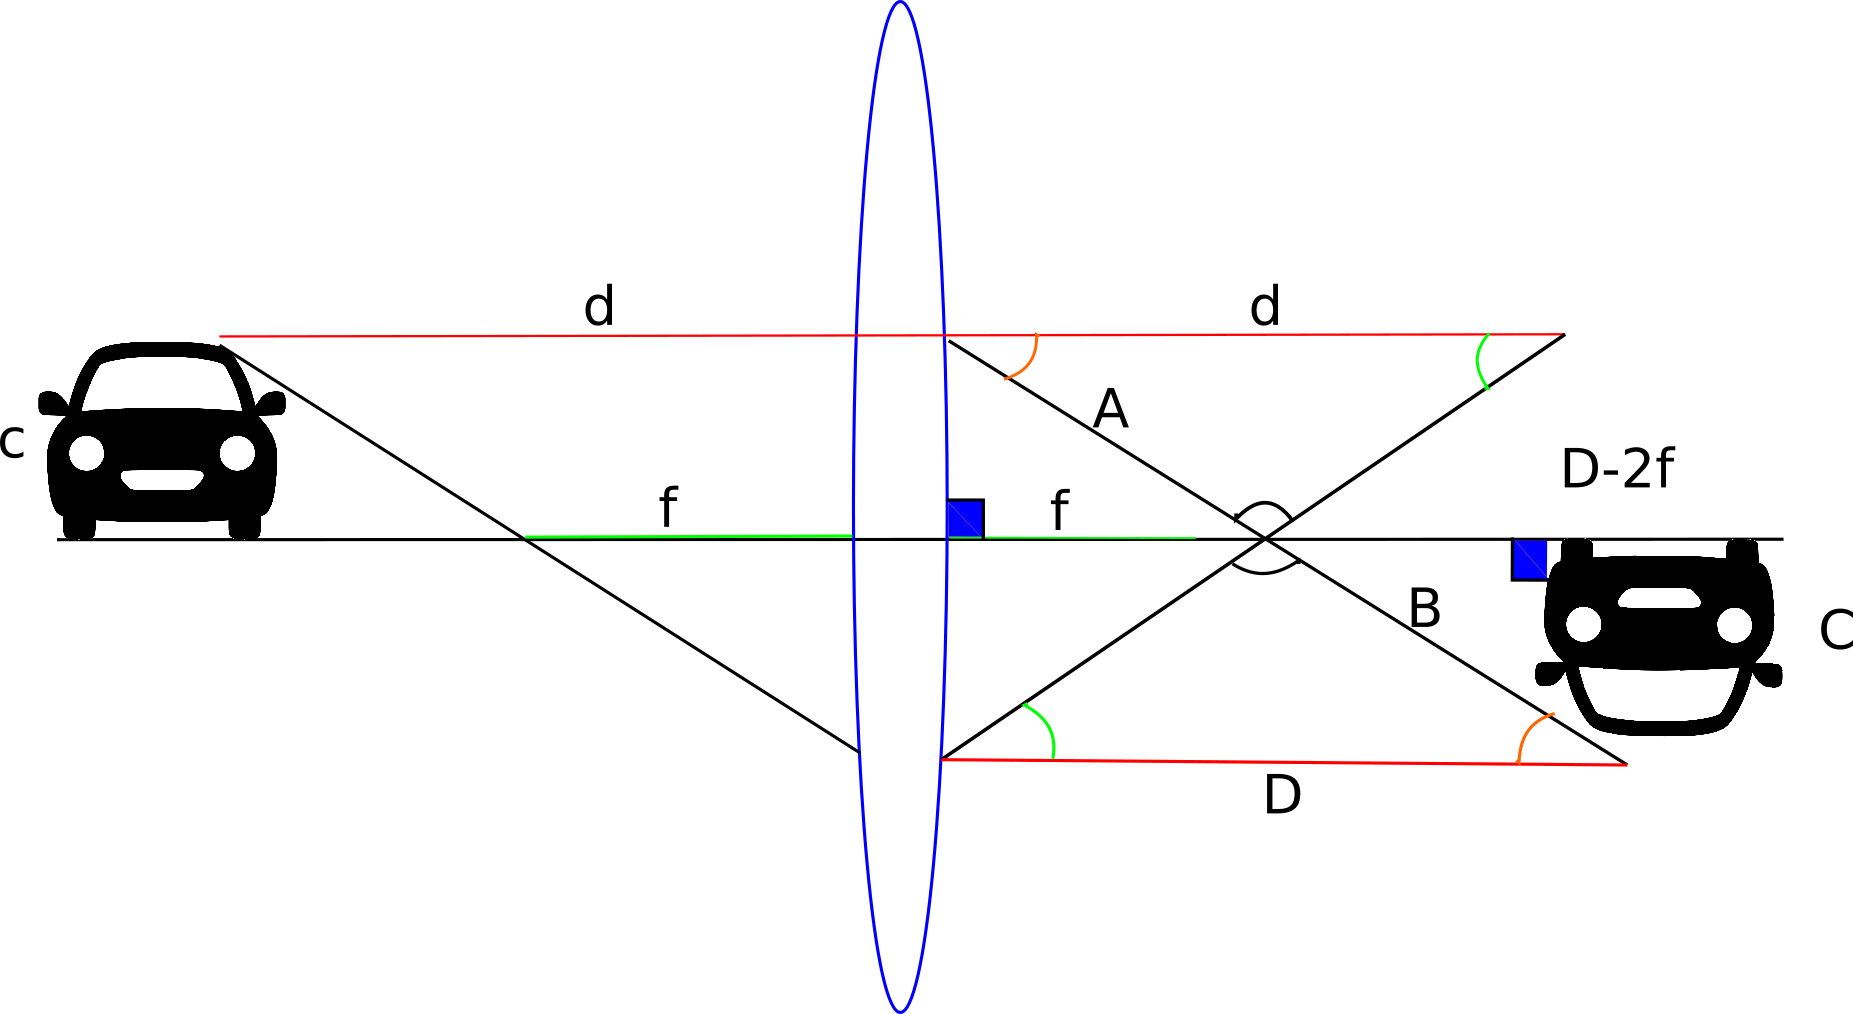
\includegraphics[width=\textwidth]{imagens/desenhando.png}
\caption{Purpose method to compute the distance of the object using cameras}
\label{fig:distance}
\end{figure}


So the red line $d$ represents the actual distance of the object from the convex length. Moreover, $D$ gives a sense of how the actual image looks. If we consider a triangle on the left side of the image (new refracted image) with base $d$ and draw a triangle similar to the left side one. So the new base of the triangle will also be done with the same perpendicular distance. If we compare the two triangles from the right side, we will see $d$, and $D$ is parallel, and the angle that creates on each side of both the triangle is opposite to each other. From which it is possible to infer that both the triangles on the right side are also similar. Now, as they are similar, the ratio of the corresponding sides will also be similar. So $\frac{d}{D} = \frac{A}{B}$. Again if we compare two triangles in the right side of the image where opposite angles are equal, and one angle of both the triangles are right angle (90$^{\circ}$ ) (dark blue area). So A and B are both hypotenuses of the similar triangle where both triangles have a right angle. So the equation is defined as:

    \begin{equation}\label{eq:meausure}
        \frac{d}{D} = \frac{A}{B} = \frac{f}{D-f},
    \end{equation}

 the focal distance is shown in (\ref{eq:focal}), 

\begin{equation}\label{eq:focal}
    \frac{1}{f} = \frac{1}{d} + \frac{1}{D},
\end{equation}

The proportional size of each image, as shown in (\ref{eq:proportion}), belong to object detection variables, as shown in (\ref{eq:distance}).


\begin{equation}
    \label{eq:proportion}
    d = f + \frac{C}{c},
\end{equation}

the focal length is computed by (\ref{eq:focal_length}), 

\begin{equation}
    \label{eq:focal_length}
    f = \frac{2\cdot 3.14 \cdot 180}{360},
\end{equation}

Finally, it is possible to predict the distance based on outputs from the predictor combined with fundamental physics in (\ref{eq:distance}), where $w$ is the width and $h$ the height of the object.

\begin{equation}
    \label{eq:distance}
    distance = \frac{2 \cdot 3.14 \cdot  180}{w + h \cdot  360}
\end{equation}



 
\section{Approach 2 - One camera with known map}\label{sub:2}

The second proposed approach is based on  \cite{mayer2016large}, where it is necessary to take the photos and label these images \cite{tzutalin6labelimg}. Its output is shown in Table \ref{tab:output_table}, and indicates the position and size of the boundary box as already defined in Figure \ref{fig:anchor}, and the real position of the car on the actual scenario, and show in Figure \ref{fig:proposal2} is shown the block diagrams and the proposed approach to predict the distance based on the known map. The subsection defines only the step regarding the estimated position based on the map because the other actions have already been described in Section \ref{sub:1}. 


\begin{figure}[H]
\centering
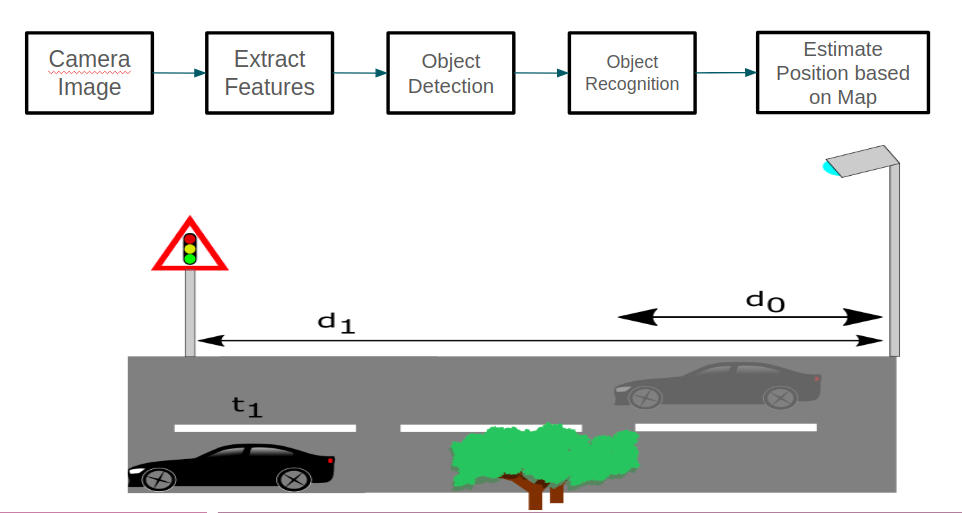
\includegraphics[width=\textwidth]{imagens/proposal2.png}
\caption{Approach using one camera with known map}
\label{fig:proposal2}
\end{figure}


\begin{table}[H]
\centering
\caption{Example of labeled values}
\begin{tabular}{llllll} 
\hline
Label        & Distance (meters) & X    & Y   & W    & H   \\
car \#1         & 4.41     & 365  & 304 & 1150 & 563  \\
car \#2        & 11.11    & 321  & 256 & 736  & 422  \\
car \#3        & 16.24    & 221  & 198 & 562  & 351  \\
car \#4        & 19.66    & 138  & 172 & 425  & 296  \\
car \#5        & 23.09    & 107  & 150 & 360  & 265  \\
road signal & 25.82    & 1226 & 6   & 1266 & 95   \\
tree        & 17.22    & 507  & 1   & 606  & 231  \\
\hline
\end{tabular}
 \label{tab:output_table}
\end{table}



\subsection{Estimate position based on map}

For this step is necessary to collect data and label this data before the start. Because based on the previous collect data, this predictor will be different compared with the estimation provided in Section \ref{sub:1}. This approach is used as an Artificial Neural Network (ANN), and the concepts of this architecture were defined in 
Subsection \ref{ml-ai}. The proposed ANN is in Figure \ref{fig:rede_neural}.


\begin{figure}[H]
\centering
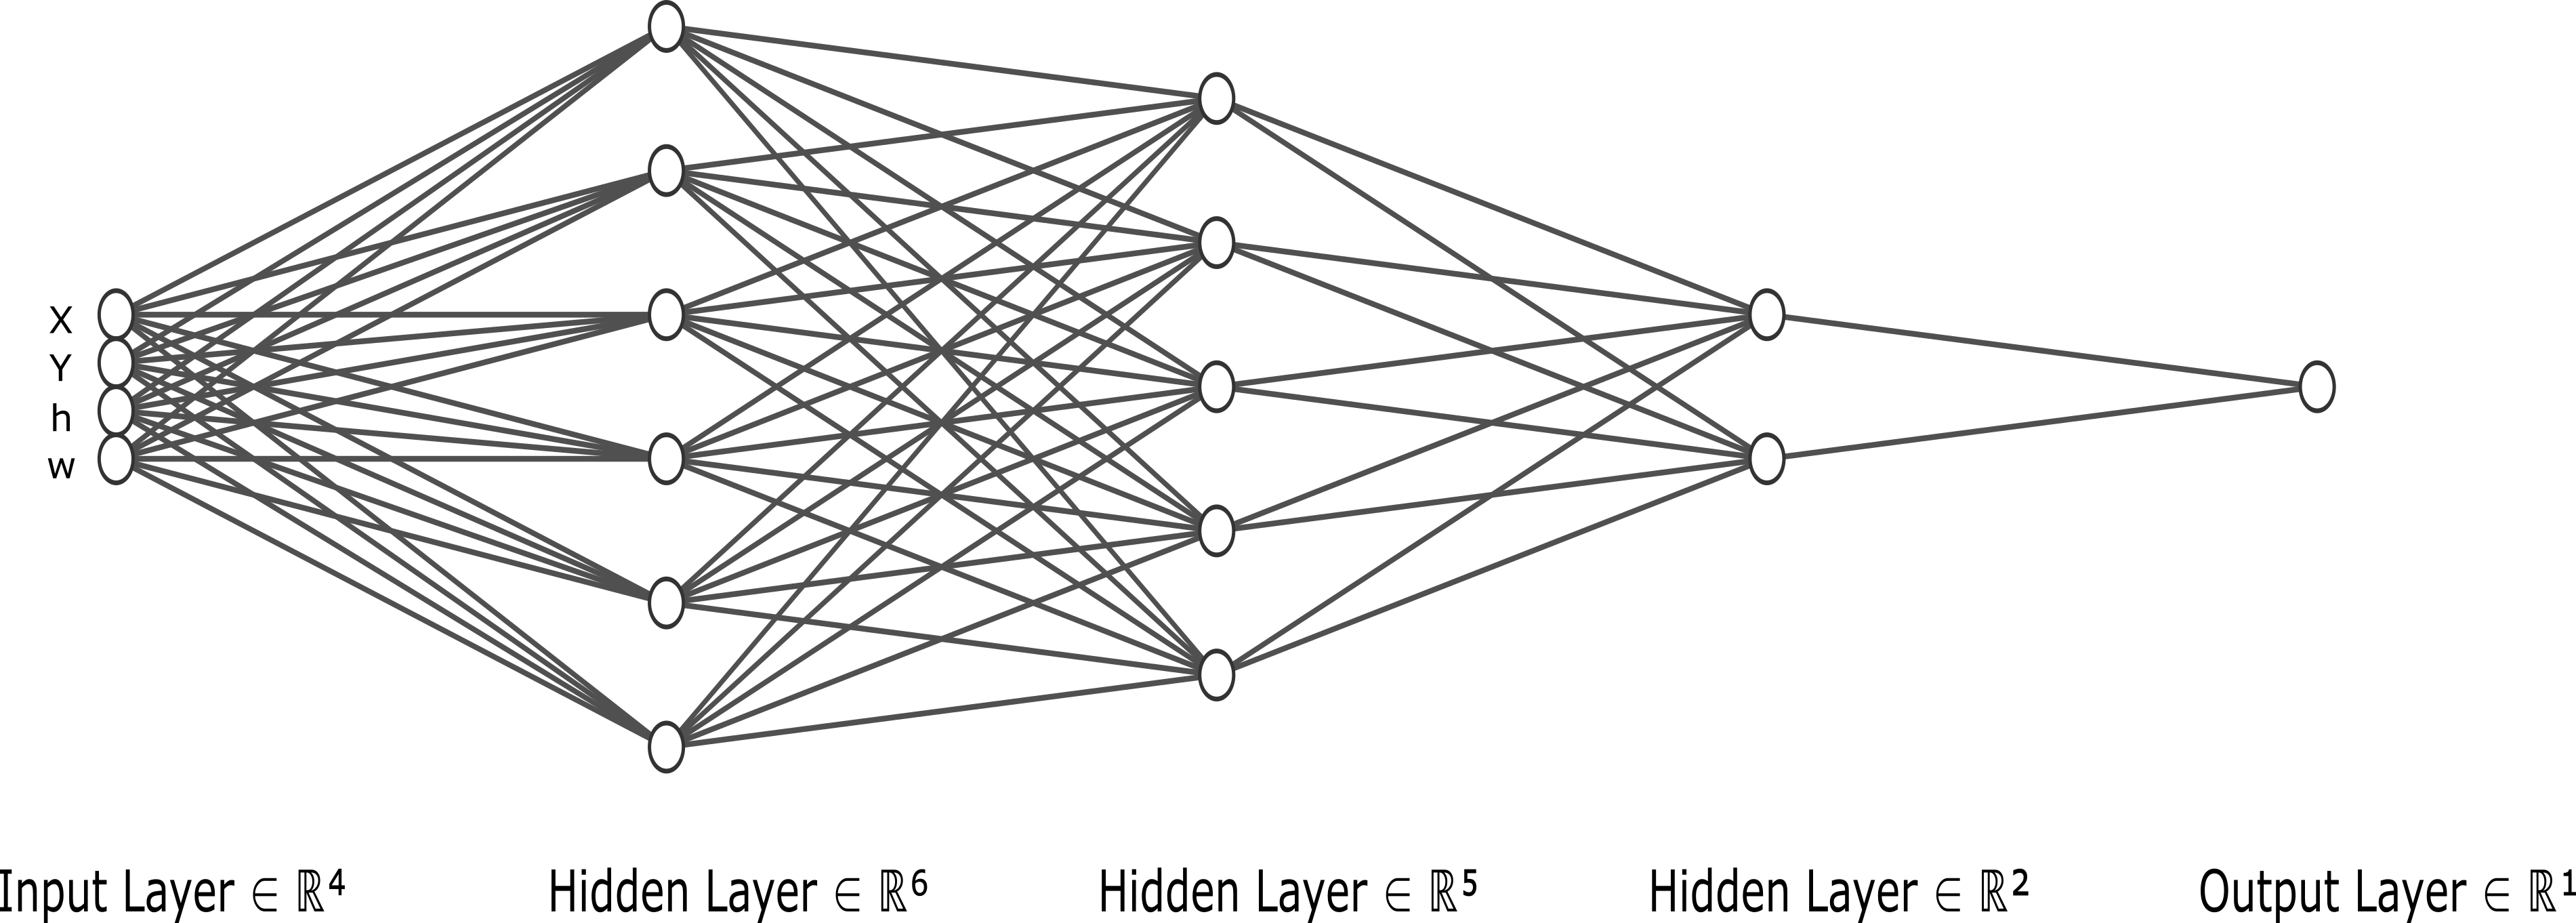
\includegraphics[width=\textwidth]{imagens/nn.png}
\caption{Neural network responsible to predict the distance of the objects based on the boundary boxes}
\label{fig:rede_neural}
\end{figure}

Additionally, this defined architecture is possible to estimate the car's distance along the scenario. An example of the labeled image is shown in Figure \ref{fig:boundary_boxes_car}. These outputs were collected from this image and saved in Extensible Markup Language (XML) and this file is used as input in the ANN. 


\begin{figure}[H]
\centering
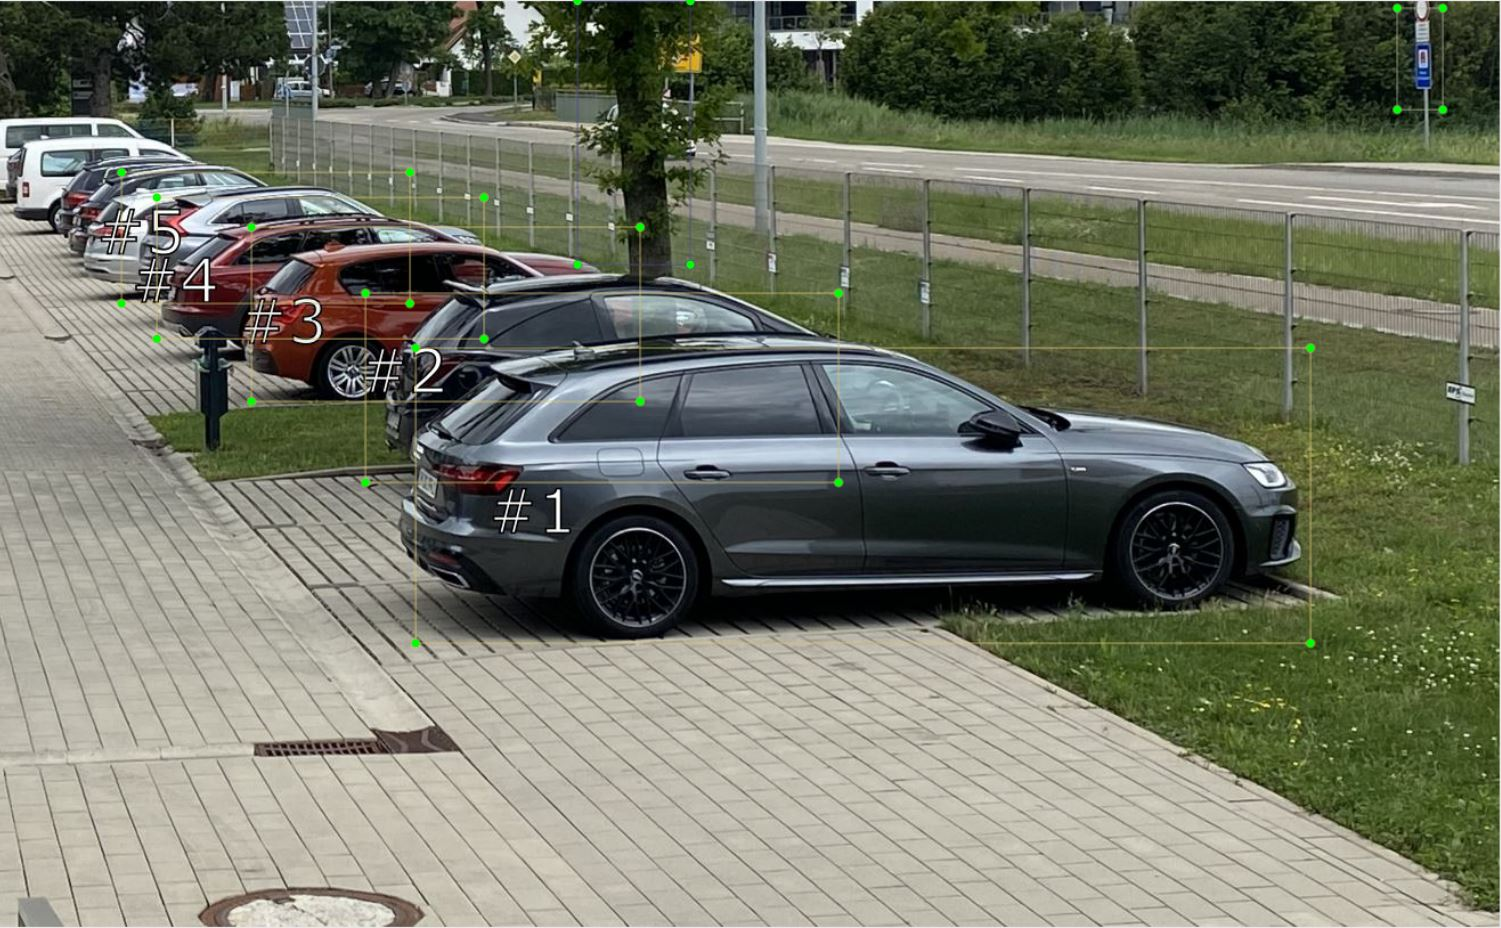
\includegraphics[scale=0.5]{imagens/boundary_boxes.JPG}
\caption{Labeled image with boundary boxes positioned in each important element of the screen}
\label{fig:boundary_boxes_car}
\end{figure}




\section{Approach 3 - Multicamera}\label{sub:3}

This approach was selected one for the construction of the framework in Subsection \ref{framework} because with this approach is possible to consider the camera's position on the test scenario. As similar in Subsection \ref{sub:2}, only the last step will be defined here because the other ones were already described in Subsection \ref{sub:1}. 


\begin{figure}[H]
\centering
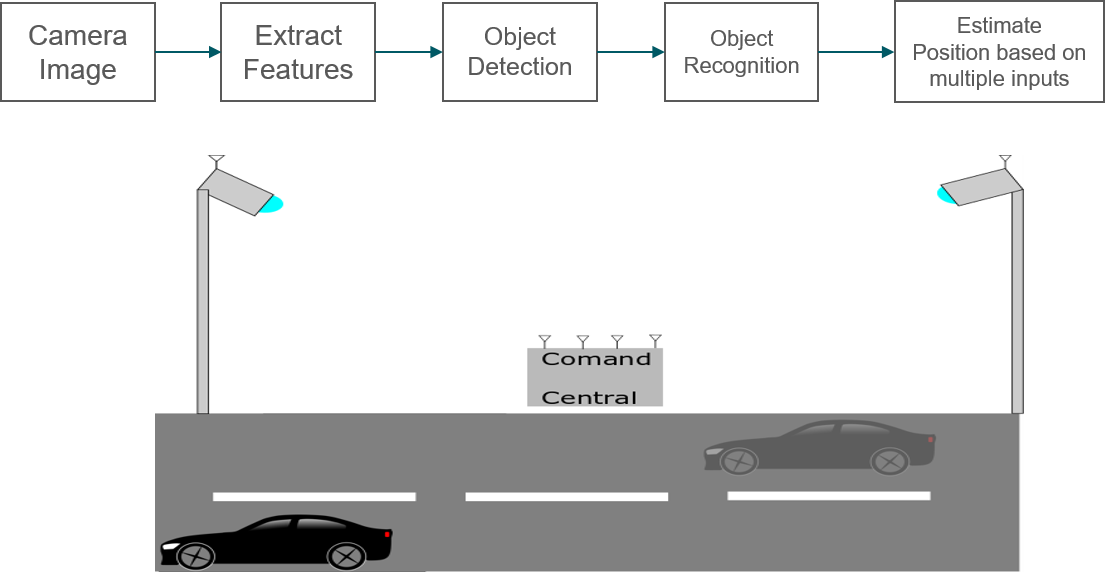
\includegraphics[scale=0.6]{imagens/proposal3.png}
\caption{Approach using multicamera}
\label{fig:proposal3}
\end{figure}

 The creation of a scenario-based in multiple cameras, forming cameras array, and a command center is responsible for merging all of the collected data and fusing this data on the database, such as the label of each object, position, and its timestamp. 

The data used on this task is provided from streams of the cameras, and they send these data to the command center via a wireless connection over the protocol IEEE 802.11. The data fusion is controlled by proxy, and it was written in Python. The distance estimation is based on the Inverse perspective mapping (IPM) and is well defined in \ref{ipm}.


\subsection{Estimate position based on multiple inputs}\label{ipm}
Inverse perspective mapping is a mathematical technique that removes the effects of a picture's distortion when transforming the image's perspective to another perspective. Despite disparity mapping, the inverse perspective mapping method requires only one camera, and this method cannot provide depth information directly ~\cite{Tuohy2010}.

The camera must be located in front of the car with an angle of \(\theta\) to down. Figure \ref{fig:ImageRelationSystem} shows the setup.

\begin{figure}[h]
\centering
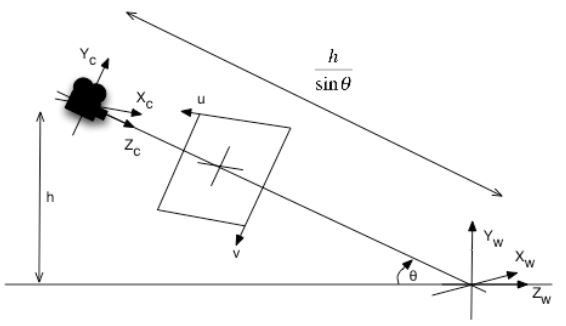
\includegraphics[scale=0.5]{imagens/Inverse Perspective Mapping.JPG}
\caption{Image coordinate system in relation to world coordinate
system.}
\label{fig:ImageRelationSystem}
\end{figure}
\par


This setup was selected based on solution of \cite{Wongsaree2018}, the mathematical background is to create top-down view, the surface road point is known as $(X_w,Y_w,Z_w)$
that projects to the image plane $(u,v)$ is a must. As disrupted in Figure \ref{fig:ImageRelationSystem}. For rotatation angle $(\theta)$, which is angle between camera and the surface, the IPM equation is based on \cite{7759904} and is shown is Equation \ref{eq:eq1}:

\begin{equation}
    (u,v,1)^T = K\cdot T \cdot K (X_w,Y_w, Z_w,1)^T
    \label{eq:eq1}
\end{equation}

where R is the rotation matrix given in the equation \ref{exp2}.
\begin{equation} \label{exp2}
R=
\begin{bmatrix}
1 & 0 & 0 & 0\\
0 & \cos{\theta} & -\sin{\theta} & 0\\
0 & \sin{\theta} & \cos{\theta} & 0\\
0 & 0 & 0 & 1
\end{bmatrix}
\end{equation}
\par

T is the translation matrix given in the equation \ref{exp3}, where h means the height of the position of the camera.
\begin{equation} \label{exp3}
T=
\begin{bmatrix}
1 & 0 & 0 & 0\\
0 & 1 & 0 & 0\\
0 & 0 & 1 & \frac{-h}{\sin{\theta}}\\
0 & 0 & 0 & 1
\end{bmatrix}
\end{equation}


\par
K is the camera parameter matrix given in (\ref{exp4}), where $f$ is the focal length of the camera, $s$ is the skew parameter, and $u_0, v_0$ are the center of the pixel of desired image size. 
\begin{equation} \label{exp4}
K =
\begin{bmatrix}
f & s & u_0 & 0\\
0 & f & v_0 & 0\\
0 & 0 & 1 & 0\\
\end{bmatrix}
\end{equation}

The Equation \ref{exp4} can be replaced using the real parameters of this test scenario and these parameters are $f = 2.92 mm, s=0, u_0=240, v_0=160$. Replacing the Equations \ref{exp2},\ref{exp3}, \ref{exp4} into the initial Equation \ref{eq:eq1}, achieving the new Equation \ref{eq:eq2}.

\begin{equation}
    \begin{bmatrix}
u\\ 
v\\ 
1
\end{bmatrix}
=\begin{bmatrix}
P_{11} & P_{12} & P_{13} & P_{14}\\ 
P_{21} & P_{22} & P_{23} & P_{24}\\ 
P_{31} & P_{32} & P_{33} & P_{34}
\end{bmatrix}
\begin{bmatrix}
X_w\\ 
Y_w\\ 
Z_w\\
1
\end{bmatrix}
\label{eq:eq2}
\end{equation}

where the matrix P was gotten from a product between K, T, and R. As is only necessary to evaluate the position of the road, so the coordinate $Y_w$ can be equal to 0, so simplifying the Equation \ref{eq:eq2}, so it is given by Equation \ref{eq:eq3}.

\begin{equation}
    \label{eq:eq3}
    \begin{bmatrix}
u\\ 
v\\ 
1
\end{bmatrix}
=\begin{bmatrix}
P_{11} & P_{12}  & P_{14}\\ 
P_{21} & P_{22}  & P_{24}\\ 
P_{31} & P_{32}  & P_{34}
\end{bmatrix}
\begin{bmatrix}
X_w\\ 
Z_w\\
1
\end{bmatrix}
\end{equation}

Based on the Equations above, it is possible to infer the Equation \ref{eq:eq4} to compute the distance from the camera until the object. 

\begin{enumerate}
    \item Calculating average intensity in the row direction from the bottom row up to top row
    \item The average intensity of each row is compared with the threshold level (obtained from the experimental), which is 50. The starting position of an indicated object is the average intensity in that row is greater than 50, and the order of that row is stored in a parameter p.
    \item The distance between object and vehicle is therefore calculated using a linear equation given in \ref{eq:eq4}.
\end{enumerate}

\begin{equation}
    \label{eq:eq4}
    d = ap+b
\end{equation}

$d$ is the distance between the camera, object, and the vehicle in meter, $p$ is the order of the row that object is detected, and $a, b$ are constants.

 
\section{Framework Architecture} \label{framework}

This section discusses how the architecture of the Subsection \ref{sub:3} is encapsulated in a software framework. This Architecture was divided into four big modules: client, model, proxy, and controller. 



\begin{figure}[H]
\centering
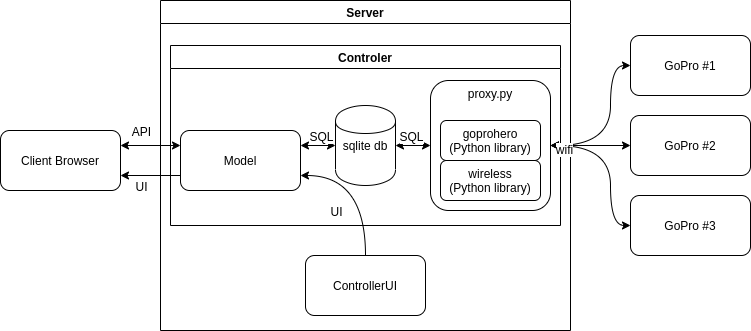
\includegraphics[scale=0.6]{imagens/diagram.png}
\caption{Architecture approach of framework}
\label{fig:framework}
\end{figure}

The first module is block 1 of Figure \ref{fig:framework} is the client, which is responsible for permitting all of the interactions with the user and allow to see the cameras making the inference and see the boundary boxes and the labels, and the distance estimation as well.

The module responsible for controlling the model is block 2 of Figure \ref{fig:framework}, and it will be expanded in Figure \ref{fig:networkBehavior}. The input data is obtained from the data provided by cameras, and the output will be saved in the database. These outputs have already been defined in Section \ref{sub:3}. 

Block 3 of Figure \ref{fig:framework} controls the usage flow of this framework and provides an abstraction layer to the usage of the database. 

In block 4 of Figure \ref{fig:framework} is the part responsible for connecting the other cameras via WIFI protocol and allows the system to connect another camera, the total amount of camera is based on the hardware available for the tests. 


Figure \ref{fig:networkBehavior} shows how the model performs the inference process along the detection time, where this Figure shows the flow of the framework in new images. For example, the camera starts to stream, and to apply the object detection on the refereed frame, then the dimension estimation network is called, and in another direction, the segmentation network is activated. After this step, it is possible to use the vehicle segmentation to detect vehicles along this way.





\begin{figure}[H]
\centering
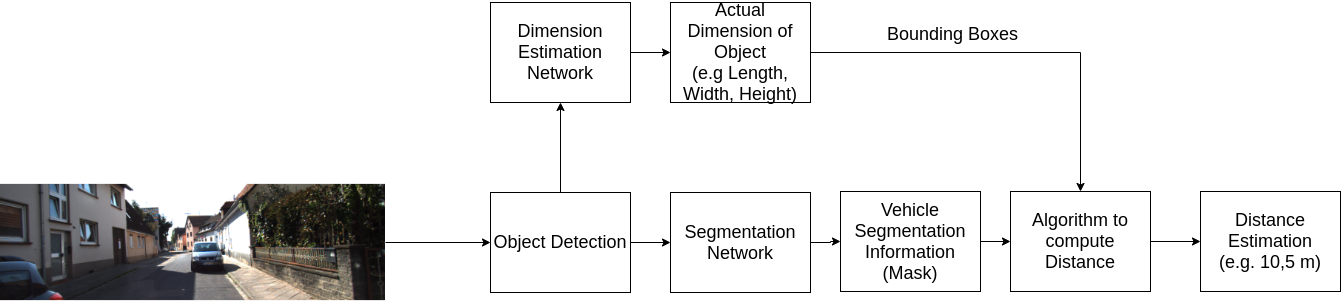
\includegraphics[width=\textwidth,height=40mm]{imagens/Network Behavior.png}
\caption{Architecture of framework based on multicameras perspective}
\label{fig:networkBehavior}
\end{figure}


Still using Figure \ref{fig:networkBehavior}, the next mutual box is the action to compute the algorithm to measure the distance of the object. In this box, the inputs are the relative position of each bounding box and the object's computed label. 

This block diagram's last action is to show the predicted distance to the user and save it into the relational database for future queries. 
\chapter{Results}
\label{capitulo5}

In this chapter, the results collected from the Chapter 4 will be discussed and analyzed. It is essential to freeze that only approach three from \ref{sub:3} was implemented into the framework, due to the goal was to work with multiple cameras and multi-view perspective.

The algorithms and the simulations was performed in a computer with this follow configuration:

\begin{itemize}
    \item Operational System Ubuntu 18.04
    \item CPU Intel core i7 7700HQ 2.80 GHz
    \item 32 GB memory RAM
    \item GPU Nvidia Geforce GTX 1050 Ti - 4 GB
\end{itemize}


The framework can perform the tests on the Audi test track, as shown in Figure \ref{fig:test_track}, but in this work, only the proof of concept of the algorithms was performed. 

\begin{figure}[H]
\centering
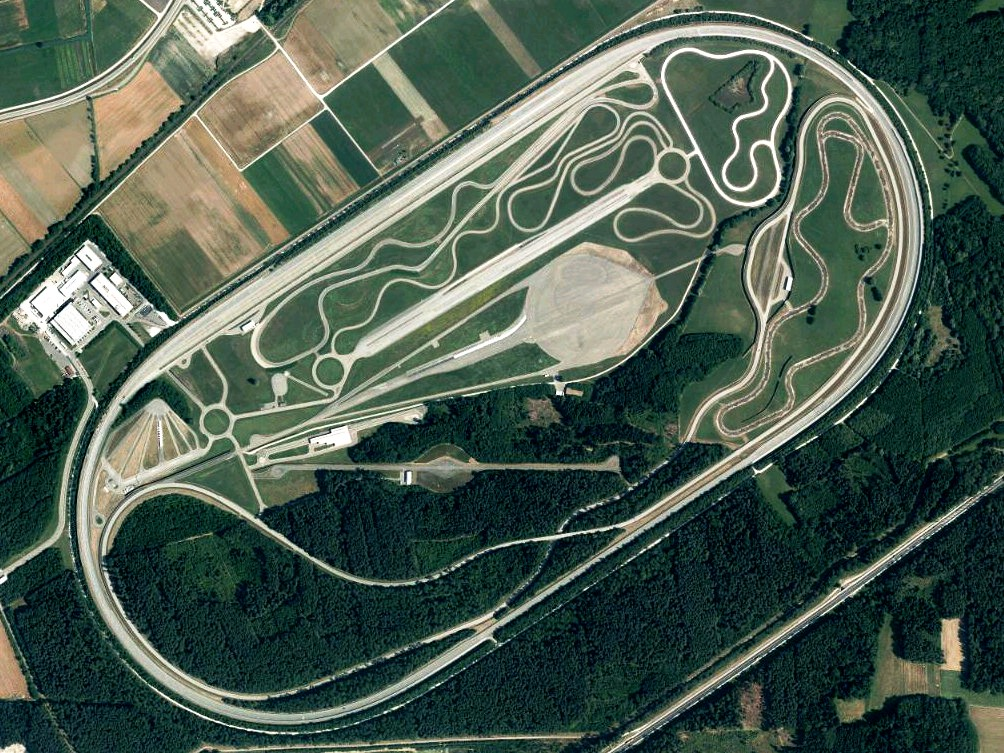
\includegraphics[scale=0.3]{imagens/testtrack.jpg}
\caption{Audi test track in eagle's view}
\label{fig:test_track}
\end{figure}


The algorithm for object detection was performed over the parking lot of the company EFS GmbH as shown in Figure \ref{fig:park}.


\begin{figure}[H]
\centering
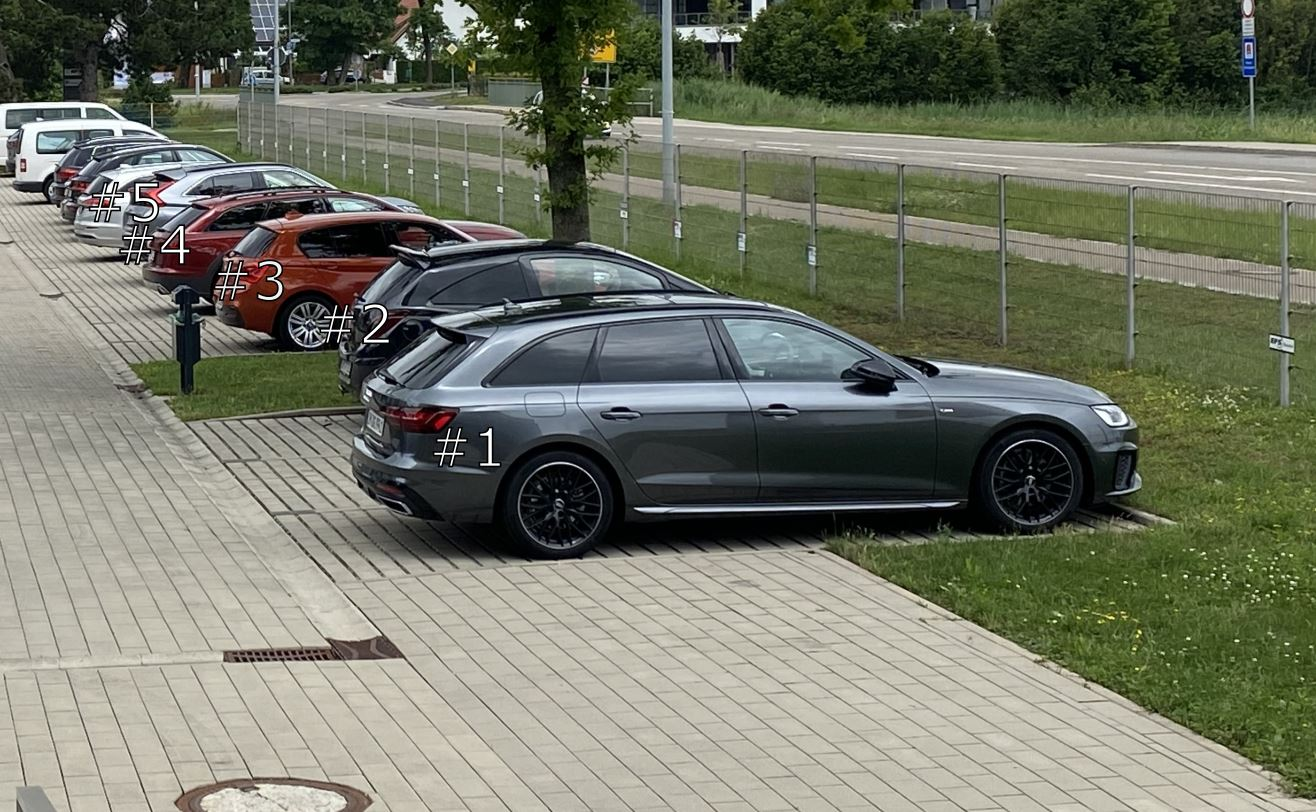
\includegraphics[scale=0.5]{imagens/park.JPG}
\caption{Position of the cars on the parking lot}
\label{fig:park}
\end{figure}

\section{Description of the test scenario}

The test scenario was built three times using different perspectives, for the first test where was necessary to use the camera calibration perspective was built using only one camera and the height of this camera does not matter to compute the distance, only a known distance, and dimensions of a known object to adjust this algorithm.

For the second scenario, some photos were taken and labeled with the known metrics to support the training step and return a useful result according to reality. 

The last approach and used in this work to built the framework was used following some principles as the cameras should be mounted at the same level, the same horizontal position,  the stream must be captured at the same time of the camera and sent to the same control center to process this data. 

The used cameras were GoPro 5, which allow building a wireless network with many cameras. 


\section{Results with camera calibration}

The results provided from approach one from \ref{sub:1} were implemented using Python 3.7 and Opencv3, and the position was computed based on the camera calibration. Equation (\ref{eq:focal_distance}) is defined as the distance used in the camera calibration, using a measurer tape and a piece of paper ($21.59$ cm x  $27.94$ cm), and this was positioned $60.96$ cm in front of the camera to take the photo.

\begin{equation}
    \label{eq:focal_distance}
    F = \frac{P\cdot D}{W}
\end{equation}

W is the width of the piece of the paper, in this case, is $27.94$ cm, D is the distance from the piece of paper to the camera, and P is the paper's measure in pixels is taken from the image. Applying the (\ref{eq:focal_distance}), the focal length (F) is $541.09$ pixels.





The results achieved with this technique is shown in Table \ref{tab:output_calibrate}. 

\begin{table}[H]
\centering
\caption{Measurements achieved with camera calibration algorithm}
\begin{tabular}{l|l} 
\toprule
Car &  Measurements      \\
\#1   & 4.05        \\
\#2   & 10.67       \\
\#3   & 15.52       \\
\#4   & 19.55       \\
\#5   & 20.08       \\
\bottomrule
\end{tabular}
\label{tab:output_calibrate}
\end{table} 



\section{Results with known map}
In this section is detailed the results of the proposal with a known map, this approach was performed using the neural network from \ref{sub:2} and the data provided from KITTI Dataset \cite{geiger2013vision}, it is essential to freeze, this approach was used only for comparison method and not to be used on the final framework. 


The results collected in this section are beneficial, as several companies and other universities are releasing the dataset as open source. There is a need to understand image manipulation, and in some cases, data from LIDAR and Radar.

The main idea of this test was to get the information from the object detection performed with the algorithm using the boundary boxes approach, collect this known information as input in the neural network, and start predicting a distance from the camera until the object. Where in Figure \ref{fig:output} is shown an example of the known KITTI dataset, it serves just as motivation for this work, the final results were not performed over this dataset. 

\begin{figure}[H]
\centering
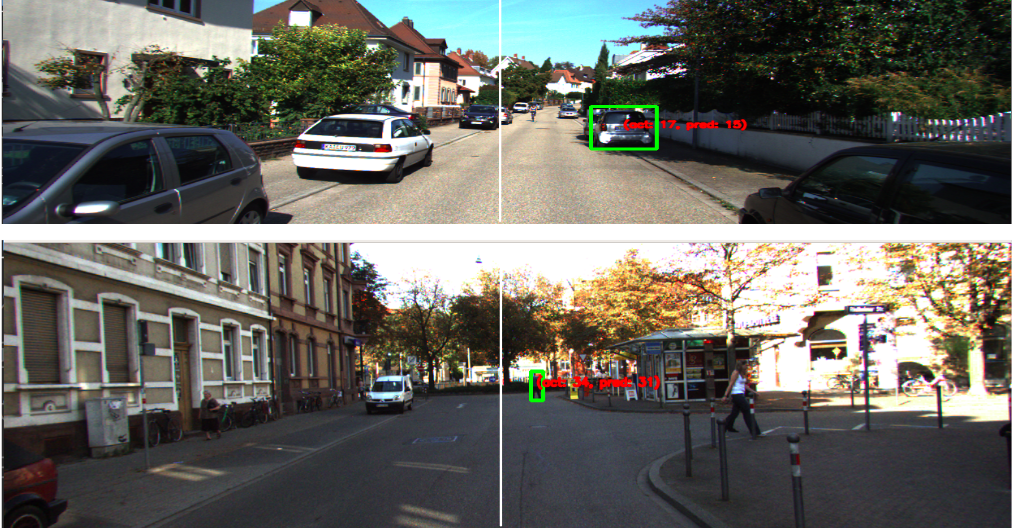
\includegraphics[width=\textwidth]{imagens/ouput.png}
\caption{Output results from framework using single stereo camera and known map}
\label{fig:output}
\end{figure}

For this approach, the output achieved from Table \ref{tab:output_table} was used for the first interaction and estimate the distance, as shown in Table \ref{tab:output_2}. These results are similar to the reality because it uses a known map, and the measurement step of these structures was performed and the labeling part.

\begin{table}[H]
\centering
\caption{Measurements achieved with camera and known map}
\begin{tabular}{l|l} 
\toprule
Car &  Measurements      \\
\#1   & 4.43        \\
\#2   & 10.98       \\
\#3   & 16.01       \\
\#4   & 18.99       \\
\#5   & 22.18       \\
\bottomrule
\end{tabular}
\label{tab:output_2}
\end{table} 


\section{Results with multi-cameras and proposed framework}


The proposed framework's algorithm predicts the objects of the whole scenario in 28 ms and has identified nine cars on the image, as shown in Figure \ref{fig:park_predict} and in Table \ref{tab:accuracy} is shown the accuracy of each prediction for each car. The output accuracies from the algorithm are shown in Table \ref{fig:framework_predict}, the low accuracies are related to the partially occluded objects, such as car two and car 6. 

The perspective of the distance, this algorithm computed this using the Inverse Perspective Mapping (IPM) combined with the Yolo Algorithm, where the perspective of distance was fused on the last fully connected layer. In Table \ref{tab:output_framework} is shown the results achieved from the perspective using two cameras. 

\begin{table}[H]
\centering
\caption{Measurements achieved with multicameras}
\begin{tabular}{l|l} 
\toprule
Car &  Measurements      \\
\#1   & 4.40        \\
\#2   & 11.05       \\
\#3   & 16.01       \\
\#4   & 19.92       \\
\#5   & 24.08       \\
\bottomrule
\end{tabular}
\label{tab:output_framework}
\end{table} 
 

In Figure \ref{fig:park_predict} was used just the model that contains the object recognition and detection using a single image and not as a stream, this test was performed to see the accuracy of the algorithm in this purpose and identify how far is possible to detect the objects in this scenario. It is necessary to note that this test previewed only five cars to detect, and the algorithm recognizes the whole cars in the scenario, each accuracy for each car of the test is available in Table \ref{tab:accuracy}.


\begin{figure}[H]
\centering
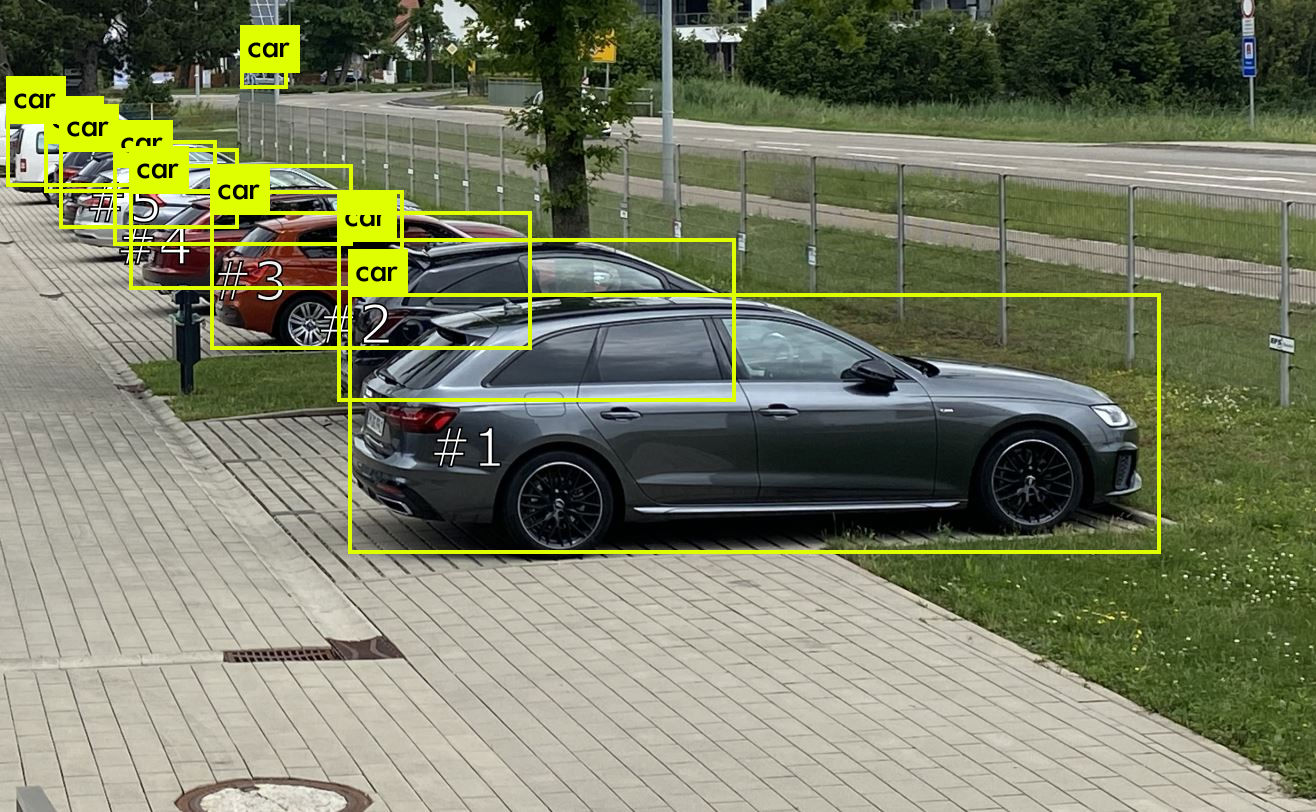
\includegraphics[scale=0.3]{imagens/predictions.jpg}
\caption{Output image with boundary boxes predictions}
\label{fig:park_predict}
\end{figure}



\begin{table}[H]
\centering
\caption{Accuracy of the proposed framework in object detector and classification}
\begin{tabular}{c|c}
\hline
Predicted Label & Accuracy \\ \hline
Car             & 91\%     \\ \hline
Car             & 31\%     \\ \hline
Car             & 96\%     \\ \hline
Car             & 94\%     \\ \hline
Car             & 95\%     \\ \hline
Car             & 98\%     \\ \hline
Car             & 47\%     \\ \hline
Car             & 97\%     \\ \hline
Car             & 98\%     \\ \hline
\end{tabular}
\label{tab:accuracy}
\end{table}



In Figure \ref{fig:framework_predict} is shown the frontend of the application of this work, it was developed using Python and Javascript to allow the browser to communicate with the model. The Python module is composed by the libraries called sockets, and it permits the communication over many cameras and shares the stream information between the cameras and the command center, it was possible because the cameras used in the tests have an internal wireless network. Too, based on it, a script with a proxy function was developed to take care of this behavior. 

The backend side of this project is described in Appendix \ref{ap:app}, where there is information about the pre-processing step, training step, object detection, and the frontend scenario as well. The network was built using the framework Pytorch \cite{paszke2019pytorch}. This script permits the Darknet abstraction to perform object detection and object recognition, and with all of this information, the step to predict the distance was combined to show the output. 

The camera 1 of the Figure \ref{fig:framework_predict} is used only to perform the boundary boxes detection, and camera two is used to perform the distance prediction. This solution was embedded in a module to work as a controller of this framework.

The experiments also led us to measure the rapidity of the multi-%cameras method by computing the number of frames treated per %second.  Fig. 9 shows that the method could treat up to 23 frames %per second. The average of frames per second through all the %experiments is 20.57 frames per second, which are enough for real-time %treatments. 

\begin{figure}[H]
\centering
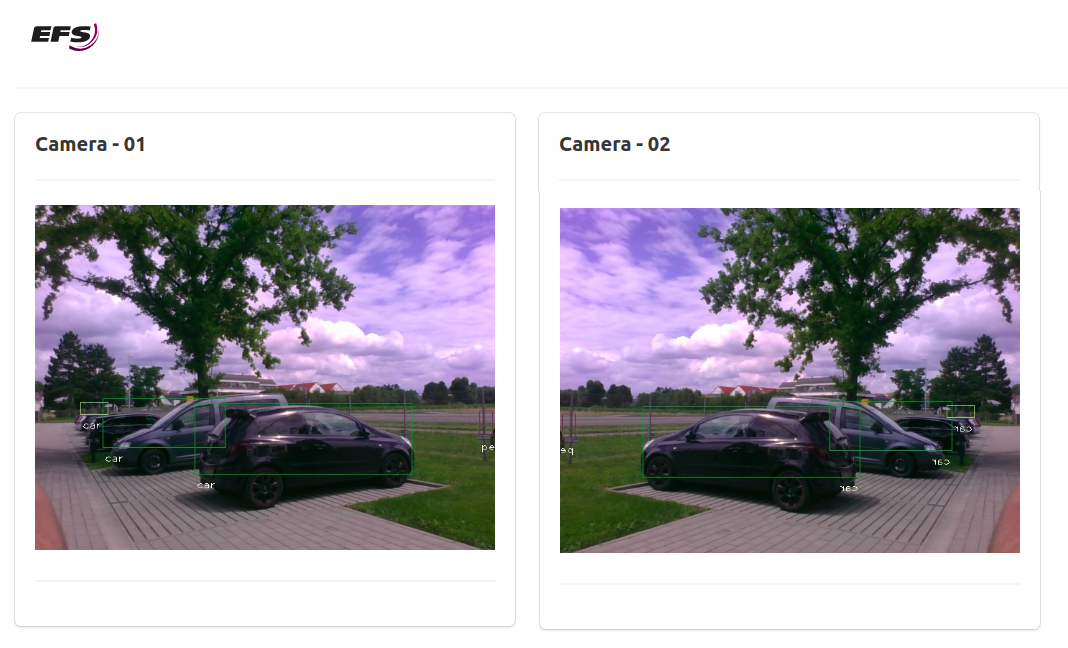
\includegraphics[scale=0.8]{imagens/output_framework.png}
\caption{Output image with predictions }
\label{fig:framework_predict}
\end{figure}



\section{Validation}

For validation purpose, it was used a commercial laser measurement as shown in Figure \ref{fig:laser_meas}, this model is known as Bosch DLE 40 Professional {\tiny{\textregistered}}. 



\begin{figure}[H]
\centering
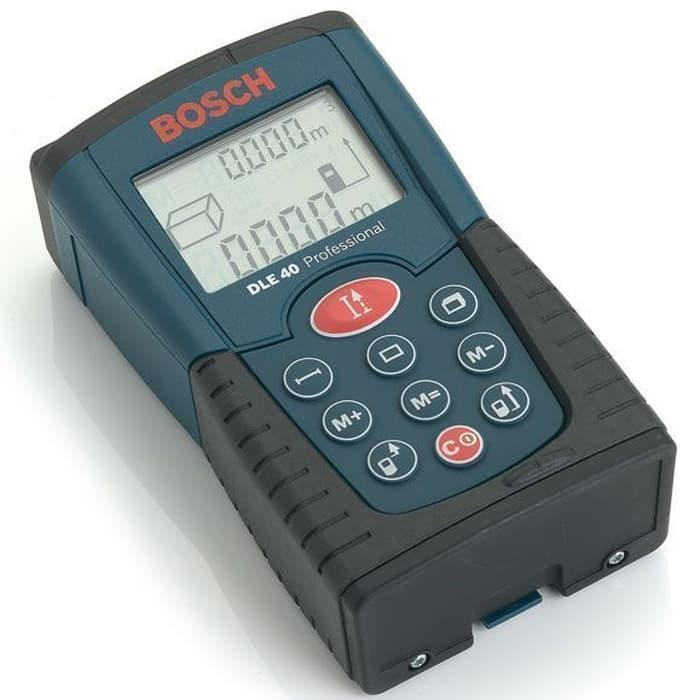
\includegraphics[scale=0.3]{imagens/trena.jpg}
\caption{Commercial laser measurer}
\label{fig:laser_meas}
\end{figure}

The current error rate is $\pm 1.5 mm$, thereby we repeated the measure three times and computed the mean and standard deviation as well. In Table \ref{tab:tab_measure} is shown the measurements with the camera positioned at $2.01$ m from the ground. Figure \ref{fig:park} is shown the position of the cars along the parking lot. The reason to measure three times is that in the manual is written that on sunny days can bias the measurement. 



\begin{table}[H]
\centering
\caption{Measurements collected with a commercial measurer}
\begin{tabular}{l|l|l|l|l} 
\toprule
Car & First measure (m) & Second measure (m) & Third measure (m) & Mean (m) \\
\#1   & 4.25          & 4.47           & 4.51           & 4.41 \\
\#2   & 11.01         & 11.21          & 11.11          & 11.11\\
\#3   & 16.12         & 16.35          & 16.26          & 16.24\\
\#4   & 19.63         & 19.69          & 19.66          & 19.66\\
\#5   & 23.08         & 23.18          & 23.01          & 23.09\\
\bottomrule
\end{tabular}
\label{tab:tab_measure}
\end{table} 


To compare the differences between the approaches and the real distance computed with the tool from Figure \ref{fig:laser_meas}. Table \ref{tab:total} was built to facilitate the visualization of these outputs. 


\begin{table}[H]
\centering
\caption{Comparison between the algorithms and real data}
\begin{tabular}{l|l|l|l|l} 
\toprule
Car & Camera Calibration (m) & Known Map (m) & Multicameras (m) & Real distance (m) \\
\#1   & 4.05          & 4.43           & \textbf{4.40 }          & 4.41 \\
\#2   & 10.67         & 10.98          & \textbf{11.05 }         & 11.11\\
\#3   & 15.52         & \textbf{16.01}          &\textbf{ 16.01 }         & 16.24\\
\#4   & \textbf{19.55}         & 18.99          & 19.92          & 19.66\\
\#5   & 20.08         & 22.18          & \textbf{24.08}          & 23.09\\
\bottomrule
\end{tabular}
\label{tab:total}
\end{table} 

It is necessary to examine the error between the real value. For this, a Python script was implement using Pandas Library \cite{mckinney2011pandas} to take care of the collected data. The error analysis was implemented to make it easier for the visualization of the best-applied technique. 

The pre-processed samples are used as input for the algorithms under text, resulting in estimations of the true position value. Results are expressed in terms of the RMSE, given by (\ref{eq:rmse}):
%
\begin{equation} \label{eq:rmse}
\text{RMSE}(f, \hat{f}) = \sqrt{\frac{1}{n_\text{samples}} \sum_{i=0}^{n_\text{samples} - 1} (f_i - \hat{f}_i)^2},
\end{equation}
%
calculated for each estimator $\hat{f}_i$, referenced either from the measurement tool of Figure \ref{fig:laser_meas} true value $f_i$ as read at the end of each measurement.

Figure \ref{fig:rmse} is shown a chart with the three proposed techniques using (\ref{eq:rmse}), where it is possible to see in specific points the multi-cameras approach was better than camera calibration.

\begin{figure}[H]
\centering
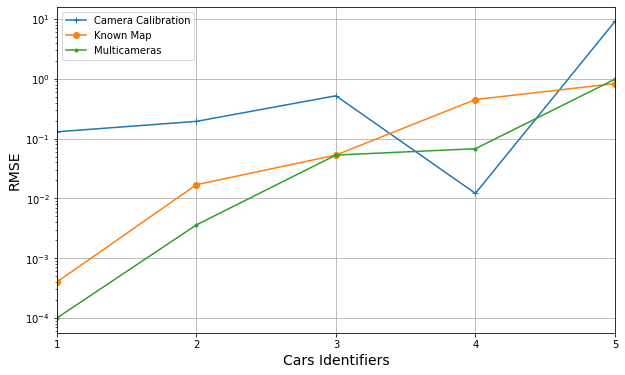
\includegraphics[scale=0.6]{imagens/plot.png}
\caption{RMSE of estimated estimate position for each algorithm for different detected car, referenced to values measured by the commercial laser measurer}
\label{fig:rmse}
\end{figure}
\chapter{Conclusion}
\label{capitulo6}


In the next years, autonomous vehicles will be a new reality, and this moment the topics regarding object detection and machine learning are the hot trends in the computer science domain. Furthermore, with this, it is necessary to improve computer vision methods to strengthen this related technology. Applying this algorithm to detect other classes of objects and perform distance measurement has improved the accuracy. 

A Real-time distance measurement method with multi-cameras for object detection on the roads is introduced in this work. The utilized method is based on using multi-cameras, which are two cameras mounted in the same horizontal position and displaced vertically by a predefined distance (the base). A vehicle detection method is performed first following two steps: hypothesis generation and hypothesis verification. 


This work also compares several state-of-the-art techniques algorithms to perform distance measurement to choose the best and faster technique. 

One of the big problems on camera arrays is the moment to put in the correct angle and high level, due to this a small filter to clear this threshold is necessary to be implemented and remove these noises. The part of calibration in the proposed technique 1 is a little bit difficult because it is needed to remember the tool error and the measurement error, and with this is possible to calibrate in the wrong way. 

It was also proved that the multi-cameras perspective combined with a high order mathematical technique is better for this work, where it is possible to divide the work of the detection into two different or more cameras. However, for our motivation and based on the current literature, the camera angle is +30 degrees, which will allow us to cover a big part of the scenario.   

\section{Future works}

According to all results collected in this work, it is possible to suggest the following approaches:

\begin{itemize}
    \item Collect data and label data to perform predictions for a specific scenario.
    \item Combine data from multiple sensors, such as LIDAR or RADAR, using data fusion approaches to increase the measurement's accuracy. 
    \item Apply other algorithms, like EfficienceDet or other novel algorithms for object detection and distance measurement.
    \item Use the proposed test in the real scenario because the algorithm was just performed in controlled sites. 
    \item Perform other mathematical approaches to reduce the dimensionality of the data.
\end{itemize}
% etc

%%%%%%%%%%%%%%%%%%%%%%%%%%%%%%%%%%%%%%%%%%%%%%%%%%%%%%%%%%%%%%%%%%%%%%%%%
% Referências bibliográficas											%
%%%%%%%%%%%%%%%%%%%%%%%%%%%%%%%%%%%%%%%%%%%%%%%%%%%%%%%%%%%%%%%%%%%%%%%%%
% \nocite{*}
% \bibliographystyle{unsrt} % use este estilo para ABNT numérico

\bibliographystyle{config/abntex2/abnt-num} % use este estilo para ABNT numérico

\renewcommand{\bibname}{BIBLIOGRAPHY}
\phantomsection
\addcontentsline{toc}{chapter}{BIBLIOGRAPHY}
\bibliography{referencias}

%%%%%%%%%%%%%%%%%%%%%%%%%%%%%%%%%%%%%%%%%%%%%%%%%%%%%%%%%%%%%%%%%%%%%%%%%
% Anexos																%
%%%%%%%%%%%%%%%%%%%%%%%%%%%%%%%%%%%%%%%%%%%%%%%%%%%%%%%%%%%%%%%%%%%%%%%%%
\anexos

\makeatletter % não retirar estes comandos
\renewcommand{\@makechapterhead}[1]{%
  {\parindent \z@ \raggedleft \setfontarial\bfseries 
        \LARGE \thechapter. \space\space 
    \uppercase{#1}\par
    \vskip 40\p@
  }
}
\makeatother


% *** Anexo I: Diagramas esquemáticos ***
\section{Code to control the app}]\label{ap:app}
\lstinputlisting[language=Python,frame=single,breaklines]{codes/app.py}

\pagebreak

\section{Code to detect the bounding boxes}\label{ap:bbox}
\lstinputlisting[language=Python,frame=single,breaklines]{codes/bbox.py}

\section{Code to control the camera}\label{ap:camera}
\lstinputlisting[language=Python,frame=single,breaklines]{codes/camera.py}

\section{Abstraction of Darknet in Pytorch}\label{ap:darknet}
\lstinputlisting[language=Python,frame=single,breaklines]{codes/darknet.py}

\pagebreak
\section{Code for data preprocessing}\label{ap:preprocess}
\lstinputlisting[language=Python,frame=single,breaklines]{codes/preprocess.py}

\pagebreak
\section{Base Template}\label{ap:template1}
\lstinputlisting[language=html,frame=single,breaklines]{codes/base.html}


\pagebreak
\section{Index Template}\label{ap:template2}
\lstinputlisting[language=html,frame=single,breaklines]{codes/index.html}


\refstepcounter{noAnexo}

% *** Anexo II: Descrição do CD ***
%\include{anexo_CD}
%\refstepcounter{noAnexo}

%\pdfbookmark[level]{text}{name}
% Acrescente mais anexos conforme julgar necessário.
\end{document}

